\documentclass[11pt,a4paper]{report}
\usepackage{luatexja-preset}
\usepackage{amsmath,amssymb,amsthm,mathtools}
\usepackage{bm}
\usepackage{graphicx}
\usepackage{float}
\usepackage[margin=25mm]{geometry}
\usepackage{hyperref}
\usepackage{xcolor}
\usepackage{array}
\hypersetup{colorlinks=true,linkcolor=blue!60!black,urlcolor=blue!50!black,citecolor=blue!50!black}
\setcounter{tocdepth}{1}
\setcounter{secnumdepth}{-1}
% MD には手書きの章番号（"第N章 …"）と節番号（"N.M …"）が入っているため、
% LaTeX 側の自動採番をオフにする（"Chapter N" 接頭辞・節番号の二重表示を防ぐ）。
\renewcommand{\chaptername}{}
\renewcommand{\thechapter}{}

\newcommand{\E}{\mathbb{E}}
\newcommand{\R}{\mathbb{R}}
\newcommand{\Var}{\mathrm{Var}}
\newcommand{\Cov}{\mathrm{Cov}}
\newcommand{\one}{\mathbf{1}}

\title{Investment Science \\ \large マルコヴィッツから連続時間最適化まで}
\author{}
\date{Version 6.0 — 主要章を大幅加筆 (手計算例・段階導出・追加図) \\ \today}

\begin{document}
\maketitle
\tableofcontents
\clearpage

% ===== 00_to_reader.md =====
\chapter{読者へ — 本書の使い方}

\section{対象読者}

本書 (v4) は \textbf{大学経済学部・経営学部・理工学部の 4 年生}（卒業研究着手レベル）を主な読者と想定する。次の前提知識を仮定する：

\begin{itemize}
\item 線形代数：行列・ベクトル演算、固有値・固有ベクトル、転置・逆行列、対称行列の対角化
\item 微積分：多変数関数の偏微分、Taylor 展開
\item 確率統計：期待値・分散・共分散、正規分布、大数の法則、中心極限定理
\item 最適化：ラグランジュ未定乗数法、凸関数の極値条件
\end{itemize}

\textbf{仮定しない}（出てきたら必要な部分だけ補足する）：
\begin{itemize}
\item 測度論的確率論、Itô 解析・確率微分方程式
\item 凸解析の双対理論、Hahn–Banach 分離定理
\item 半正定値計画 (SDP)、Wasserstein 距離、自由確率論
\end{itemize}

\section{本書の編集方針}

\begin{enumerate}
\item \textbf{証明の代わりに「直観 → 数値例 → 結論」} を基本にする。完全な厳密証明は参考文献にゆずる。
\item \textbf{数学補足ボックス} で必要な道具（ラグランジュ法、二次形式、Euler の同次関数定理 など）を本文の流れを止めずに復習する。
\item \textbf{実務注意ボックス} で「教科書通りに動かない理由」を端的に示す。
\item 各章末に \textbf{「上級学習への道標」} を 2-3 行で添え、大学院や専門研究につなぐ。
\end{enumerate}

\section{ボックスの種類と意味}

本書では 4 種類のボックスを使い分ける：

\begin{center}
\begin{tabular}{|l|l|l|}
\hline
ボックス & 役割 & 例 \\ \hline
🎯 \textbf{直観 box} & 数式の前に「何が起きているか」を言葉で説明 & 「分散投資が機能する直観」 \\ \hline
📐 \textbf{数学補足 box} & 本文で使う数学道具の最小限の復習 & 「ラグランジュ未定乗数法」 \\ \hline
⚠️ \textbf{実務注意 box} & 教科書理論が現場で使えない／使い方を間違えやすい点 & 「ベータは推定期間で変わる」 \\ \hline
📜 \textbf{歴史 note} & 理論が生まれた背景・経緯（読み飛ばし可） & 「CAPM は Markowitz の均衡版」 \\ \hline
\end{tabular}
\end{center}

\section{章ごとの読み進め方ガイド}

\begin{itemize}
\item \textbf{第 0 章} は記号・前提知識の確認用。既に知っていれば skim でよい。
\item \textbf{第 1–4 章} は基礎中の基礎。順番に読むこと。
\item \textbf{第 5 章（APT）} から \textbf{第 9 章（Black–Litterman）} は独立に読める。興味のあるところから。
\item \textbf{第 10 章（Merton 連続時間）} は本書の「最も背伸びした章」。難しければ § 10.1–10.3 だけ読んで先に進む。
\item \textbf{第 11–16 章} は応用編。実証研究や運用に関心がある読者向け。
\item \textbf{第 17 章} は演習。各問題に難易度ラベル付き：
\item ★ 計算問題（手で解ける）
\item ★★ シミュレーション問題（Python、\textbf{選択}）
\item ★★★ 考察問題（言葉で答える）
\end{itemize}

\section{演習問題の活用について}

\begin{itemize}
\item \textbf{★（手計算）は必修}：理論を「式で動かす」訓練。
\item \textbf{★★（Python）は選択}：プログラミング前提があれば取り組む。ない読者は本書を読み終えた後の発展課題として置いておくこと。
\item \textbf{★★★（考察）は卒研の準備}：採点基準（評価軸・含むべき論点）を本文中で明示する。
\end{itemize}

\section{大学院に進む読者へ}

本書は学部向けに簡略化しているため、各章末に「上級学習への道標」を置いた。例えば：

\begin{itemize}
\item 第 8 章末：\textbf{Artzner et al. (1999) の coherent risk measure の双対表現} — 凸解析と Hahn–Banach 分離が必要。
\item 第 10 章末：\textbf{Merton 問題の厳密な動的計画原理と HJB 方程式} — Karatzas–Shreve \emph{Brownian Motion and Stochastic Calculus}。
\item 第 12 章末：\textbf{Marčenko–Pastur 分布の Stieltjes 変換による導出と Ledoit–Wolf 非線形縮小} — Bun–Bouchaud–Potters \emph{Physics Reports} (2017)。
\item 第 13 章末：\textbf{Wasserstein 距離による分布ロバスト最適化} — Mohajerin Esfahani \& Kuhn (2018)。
\end{itemize}

これらは大学院修士課程の専門科目で扱われる内容である。本書はそこへの \textbf{正しい入口} を提供することを目的とする。

\noindent\hrulefill

% ===== 00_preliminaries.md =====
\chapter{第0章 記号と準備}

\begin{quote}
🎯 \textbf{この章で答える問い}
- リターンを \textbf{ベクトル・行列で書く} と何が嬉しいか。
- 「分散共分散行列が正定値」とは何を意味するのか。
- \textbf{ラグランジュ未定乗数法} はなぜ平均分散最適化の中心道具なのか。

📐 \textbf{前提知識チェック}
- 行列と転置（$A^\top$、$AB$ の計算）
- 固有値・固有ベクトル（$Av = \lambda v$）
- 期待値と分散の線形性
- 多変数関数の偏微分とラグランジュ未定乗数法

🔑 \textbf{主要記号}：$R$ リターンベクトル、$\mu = \mathbb{E}[R]$、$\Sigma = \mathrm{Cov}(R)$、$w$ ポートフォリオ重み、$\mathbf{1} = (1, \dots, 1)^\top$、$r_f$ 無リスク利子率。
\end{quote}

\section{0.1 ベクトル・行列の基本}

$n$ 種類の危険資産が市場に存在するとし、各資産 $i$ の確率的なリターンを $R_i$ で表す。リターンベクトル $R = (R_1, \dots, R_n)^\top$ について

\[ \mu := \mathbb{E}[R] \in \mathbb{R}^n, \qquad \Sigma := \mathrm{Cov}(R) = \mathbb{E}[(R-\mu)(R-\mu)^\top] \in \mathbb{R}^{n\times n} \]

を定義する。$\Sigma$ は対称半正定値であり、本書では特に断りがない限り \textbf{正定値（$\Sigma \succ 0$）} を仮定する（資産間に完全な線形従属がない、という非縮退条件に対応）。

ポートフォリオは重みベクトル $w \in \mathbb{R}^n$ で表し、ポートフォリオリターンは

\[ R_w := w^\top R, \qquad \mathbb{E}[R_w] = w^\top \mu, \qquad \mathrm{Var}(R_w) = w^\top \Sigma w. \]

完全投資制約は $\mathbf{1}^\top w = 1$、ショート禁止制約は $w \ge 0$ である。

\section{0.2 正定値行列に関する補題}

\textbf{補題 0.1}（コーシー・シュワルツ型不等式） $\Sigma \succ 0$ のとき、任意の $x, y \in \mathbb{R}^n$ に対し \[ (x^\top \Sigma y)^2 \le (x^\top \Sigma x)(y^\top \Sigma y), \] 等号は $x$ と $y$ が線形従属のとき。

\emph{証明方針}：$\langle x, y\rangle_\Sigma := x^\top \Sigma y$ は $\Sigma \succ 0$ より内積となるため、通常のコーシー・シュワルツが適用できる。$\square$

\textbf{補題 0.2} $\Sigma \succ 0$ ならば $\Sigma^{-1}$ も対称正定値であり、二次形式 $f(w) = \tfrac{1}{2} w^\top \Sigma w$ は狭義凸である。

\section{0.3 制約付き二次計画}

平均分散分析の中核は次の問題である。

\[ \min_{w \in \mathbb{R}^n} \quad \tfrac{1}{2}\, w^\top \Sigma w \quad \text{s.t.} \quad A w = b \]

ここで $A \in \mathbb{R}^{m \times n}$（$m \le n$、$A$ は行フルランク）、$b \in \mathbb{R}^m$。

\textbf{定理 0.3}（一般二次計画の解） 最適解は一意に \[ w^\star = \Sigma^{-1} A^\top (A \Sigma^{-1} A^\top)^{-1} b \] で与えられる。

\emph{証明方針}：Lagrangian $L(w, \lambda) = \tfrac{1}{2} w^\top \Sigma w - \lambda^\top (Aw - b)$ について $\partial_w L = 0$ より $w = \Sigma^{-1} A^\top \lambda$、これを制約 $Aw = b$ に代入して $\lambda$ を解き、再代入する。$\Sigma$ 正定値より目的関数は狭義凸、よって停留点が唯一の大域最小。$\square$

この公式は \textbf{第2章で効率的フロンティアの閉形表現} を導く際に繰り返し用いられる。

\section{0.4 凸性・期待効用に向けた補題}

\textbf{Jensen の不等式}：$u$ が凹関数のとき $\mathbb{E}[u(X)] \le u(\mathbb{E}[X])$。等号は $X$ が定数のとき（$u$ が狭義凹ならば）。

\textbf{確率変数の絶対連続変換}：密度 $p$ を持つ $X$ に対し $Y = g(X)$ の密度は変数変換公式で得られる。リスク尺度の章で用いる。

\section{0.5 確率過程の最小限の準備（第10章で詳述）}

\begin{itemize}
\item 標準ブラウン運動 $W_t$、Itô 積分、Itô の公式
\item 幾何ブラウン運動：$dS_t = \mu S_t \, dt + \sigma S_t \, dW_t$
\item 動的計画原理と Hamilton–Jacobi–Bellman 方程式
\end{itemize}

これらは該当章で再導入する。

\section{0.6 数学補足ボックス（本書を通して使うミニ復習）}

\subsection{📐 数学補足 box：ラグランジュ未定乗数法}

制約 $g(x) = 0$ の下で $f(x)$ を最大化したいとき、ラグランジアン \[ L(x, \lambda) = f(x) - \lambda \cdot g(x) \] を作り、$\partial L / \partial x = 0$, $\partial L / \partial \lambda = 0$ を解けばよい。複数制約 $g_1(x) = 0, \dots, g_m(x) = 0$ なら乗数も $\lambda_1, \dots, \lambda_m$ と複数になる。

\textbf{直観}：制約面上で停留点であるためには、$f$ の勾配が制約の勾配の線形結合に等しくなければならない。乗数 $\lambda$ は「制約を 1 単位緩めたときの目的関数の改善量」（\textbf{シャドウプライス}）として解釈できる。

平均分散最適化では $f = -\tfrac{1}{2}w^\top \Sigma w$（最小化なので符号は逆）、制約は $w^\top \mu = \mu_P$、$\mathbf{1}^\top w = 1$ の 2 本。

\subsection{📐 数学補足 box：行列の正定値性が意味すること}

対称行列 $A$ が \textbf{正定値} とは、すべての非零ベクトル $x$ で $x^\top A x > 0$ となること。同値な条件：

\begin{enumerate}
\item 固有値がすべて正
\item 逆行列 $A^{-1}$ が存在し、これも正定値
\item Cholesky 分解 $A = L L^\top$（$L$ は下三角行列）が存在
\end{enumerate}

\textbf{金融的意味}：共分散行列 $\Sigma$ の正定値性は「\textbf{どのポートフォリオを組んでも分散が必ず正}」、すなわち「リスクゼロを実現する非自明なポートフォリオは存在しない」ことを意味する。資産間に完全な裁定機会がない条件と密接に関係する。

\subsection{📐 数学補足 box：Euler の同次関数定理}

$f(\lambda x) = \lambda^k f(x)$ を満たす関数を \textbf{$k$ 次同次} と呼ぶ。$k = 1$（1 次同次）なら \[ f(x) = \sum_i x_i \frac{\partial f}{\partial x_i}. \]

\textbf{応用}：ポートフォリオ標準偏差 $\sigma_P(w) = \sqrt{w^\top \Sigma w}$ は重み $w$ について 1 次同次。よって \[ \sigma_P(w) = \sum_i w_i \frac{\partial \sigma_P}{\partial w_i} \] と \textbf{リスク寄与の和} に分解できる。第14章のリスクパリティの基礎となる。

\begin{figure}[H]
\centering
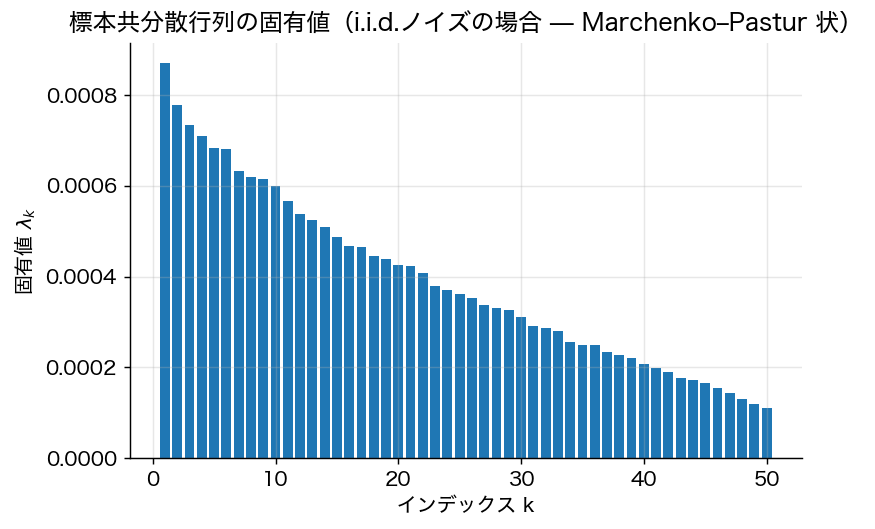
\includegraphics[width=0.85\linewidth]{figures/eigenspectrum.png}
\caption{共分散行列の固有値スペクトル例（標本$T=200$、$n=50$、i.i.d.ノイズ）。最大固有値は集中・最小固有値は $0$ に近く、最適化はこの「小さい固有値方向」を増幅するため推定誤差問題が深刻になる。}
\end{figure}

\noindent\hrulefill

% ===== 01_markowitz_basics.md =====
\chapter{第1章 Markowitz の平均分散分析}

\begin{quote}
🎯 \textbf{この章で答える問い}
- 「投資のリスク」を \textbf{分散} で測ると何が決まるのか。
- \textbf{分散投資} はなぜ機能するのか — 直観だけでなく数式で。
- 最適ポートフォリオはどんな形で書けるか — 閉じた式で。

📐 \textbf{使う数学}：ラグランジュ未定乗数法、行列の逆行列、二次形式の最小化。

🔑 \textbf{主要結果}：効率的ポートフォリオは $w^\star = \alpha_1 \Sigma^{-1} \mathbf{1} + \alpha_2 \Sigma^{-1} \mu$ と書ける。すなわち \textbf{2 つの基底ベクトルだけ} で表現できる。
\end{quote}

\begin{quote}
\emph{"Diversification is both observed and sensible; a rule of behavior which does not imply the superiority of diversification must be rejected both as a hypothesis and as a maxim."}  — H. M. Markowitz (1952)
\end{quote}

\section{1.1 問題設定}

投資家が $n$ 個の危険資産に資金を配分する。リターン $R$ について $\mu = \mathbb{E}[R]$, $\Sigma = \mathrm{Cov}(R) \succ 0$ を所与とする。ポートフォリオ $w$ の

\begin{itemize}
\item 期待リターン：$\mathbb{E}[R_w] = w^\top \mu$
\item 分散（リスク）：$\mathrm{Var}(R_w) = w^\top \Sigma w$
\end{itemize}

Markowitz の中心思想は次の二つ：

\begin{enumerate}
\item \textbf{「リスク」を分散で測る}。リターンの確率分布は平均と分散の二つの値だけで（投資家にとって）十分である。
\item \textbf{平均と分散のトレードオフを明示的に最適化する}。これにより「分散投資の価値」が定量化される。
\end{enumerate}

\section{1.2 平均分散効率性}

\textbf{定義 1.1}（平均分散効率的ポートフォリオ） ポートフォリオ $w^\star$ が \textbf{効率的（efficient）} であるとは、これと同じか高い期待リターンを持ち、かつ厳密に小さい分散を持つ別のポートフォリオが存在しないことをいう。すなわち以下の問題の解として特徴付けられる：

\[ \min_{w \in \mathbb{R}^n} \tfrac{1}{2} w^\top \Sigma w \quad \text{s.t.}\quad w^\top \mu = \mu_P,\ \mathbf{1}^\top w = 1. \tag{P} \]

\section{1.3 効率的ポートフォリオの陽な表現}

問題 (P) は第0章の二次計画の枠組みに当てはまる。$A = \begin{pmatrix} \mu^\top \\ \mathbf{1}^\top \end{pmatrix}$, $b = \begin{pmatrix} \mu_P \\ 1 \end{pmatrix}$ とおき、次の \textbf{基本スカラー量} を定義する：

\[ A_0 := \mathbf{1}^\top \Sigma^{-1} \mathbf{1}, \qquad B_0 := \mathbf{1}^\top \Sigma^{-1} \mu, \qquad C_0 := \mu^\top \Sigma^{-1} \mu, \qquad D_0 := A_0 C_0 - B_0^2. \]

\textbf{補題 1.2} $\mu$ が $\mathbf{1}$ と平行でない（つまり全資産の期待リターンが同一でない）とき $D_0 > 0$。

\emph{証明方針}：$\Sigma^{-1} \succ 0$ より $(x, y) \mapsto x^\top \Sigma^{-1} y$ は内積、コーシー・シュワルツより $B_0^2 = (\mathbf{1}^\top \Sigma^{-1} \mu)^2 \le A_0 C_0$。等号は $\mu \parallel \mathbf{1}$ のときのみ。$\square$

\textbf{定理 1.3}（効率的ポートフォリオの陽な解） 問題 (P) の最適解は \[ \boxed{\; w^\star(\mu_P) = \frac{C_0 - B_0 \mu_P}{D_0}\, \Sigma^{-1} \mathbf{1} + \frac{A_0 \mu_P - B_0}{D_0}\, \Sigma^{-1} \mu \;} \] で与えられ、対応する最小分散は \[ \sigma_P^2(\mu_P) = w^{\star\top} \Sigma w^\star = \frac{A_0 \mu_P^2 - 2 B_0 \mu_P + C_0}{D_0}. \tag{1.1} \]

\emph{証明方針}：Lagrangian $L(w, \lambda_1, \lambda_2) = \tfrac{1}{2} w^\top \Sigma w - \lambda_1 (w^\top \mu - \mu_P) - \lambda_2(\mathbf{1}^\top w - 1)$。
\begin{itemize}
\item $\partial_w L = 0 \Rightarrow w = \lambda_1 \Sigma^{-1}\mu + \lambda_2 \Sigma^{-1}\mathbf{1}$。
\item 制約 $w^\top \mu = \mu_P, \mathbf{1}^\top w = 1$ に代入し $\lambda_1, \lambda_2$ について連立一次方程式を解く：
\end{itemize}
\[ \begin{pmatrix} C_0 & B_0 \\ B_0 & A_0 \end{pmatrix} \begin{pmatrix} \lambda_1 \\ \lambda_2 \end{pmatrix} = \begin{pmatrix} \mu_P \\ 1 \end{pmatrix}. \]
\begin{itemize}
\item 行列式 $D_0$ より $\lambda_1 = (A_0 \mu_P - B_0)/D_0$、$\lambda_2 = (C_0 - B_0 \mu_P)/D_0$。
\item 分散は $w^{\star\top}\Sigma w^\star = \lambda_1 \mu_P + \lambda_2$ より整理して (1.1) を得る。$\square$
\end{itemize}

\textbf{系 1.4}（大域最小分散ポートフォリオ；GMV） (1.1) を $\mu_P$ について最小化すると $\mu_P^{\rm GMV} = B_0 / A_0$、対応する重みは \[ w^{\rm GMV} = \frac{\Sigma^{-1} \mathbf{1}}{\mathbf{1}^\top \Sigma^{-1} \mathbf{1}}, \qquad \sigma_{\rm GMV}^2 = \frac{1}{A_0}. \]

\section{1.4 分散投資が機能する仕組み（直観）}

\begin{quote}
🎯 \textbf{直観 box：なぜ「卵を一つのカゴに盛るな」が数式で正当化されるのか}

1 つの資産だけ持つと、その資産特有のリスクをそのまま被る。複数の資産を持つと、\textbf{個別ショックは部分的に相殺} される。数式では「相殺」は \textbf{共分散項} $w_1 w_2 \rho \sigma_1 \sigma_2$ に現れる。$\rho < 1$（完全相関でない）なら、組合せ全体の分散は重み付き平均より \textbf{必ず小さく} できる。これが Markowitz の核心メッセージである。
\end{quote}

\subsection{1.4.1 二資産モデルの完全導出}

2 資産 $A, B$、重み $w_A = w$, $w_B = 1 - w$ とする。期待値は単純に \[ \mathbb{E}[R_P] = w \mu_A + (1 - w) \mu_B. \] 分散は \[ \mathrm{Var}(R_P) = w^2 \sigma_A^2 + (1 - w)^2 \sigma_B^2 + 2 w (1 - w) \rho \sigma_A \sigma_B. \]

これを \textbf{最小化する $w$} を求めよう。$\partial \mathrm{Var}/\partial w = 0$ より \[ 2 w \sigma_A^2 - 2(1 - w) \sigma_B^2 + 2(1 - 2w) \rho \sigma_A \sigma_B = 0. \] 整理して \[ \boxed{\; w^{\rm GMV}_A = \frac{\sigma_B^2 - \rho \sigma_A \sigma_B}{\sigma_A^2 + \sigma_B^2 - 2 \rho \sigma_A \sigma_B}, \quad w^{\rm GMV}_B = 1 - w^{\rm GMV}_A.\;} \]

\textbf{数値例}：$\sigma_A = 0.2, \sigma_B = 0.3, \rho = 0.3$ なら \[ w^{\rm GMV}_A = \frac{0.09 - 0.3 \cdot 0.06}{0.04 + 0.09 - 2 \cdot 0.3 \cdot 0.06} = \frac{0.072}{0.094} \approx 0.766. \] すなわち低ボラ資産 $A$ に約 77\% 配分。これが GMV の本質：\textbf{ボラの低い方を多く持つ}。ただし $\rho$ が負なら、ボラが高くても多めに持つこともある（ヘッジ効果）。

\textbf{特殊ケース：$\rho = -1$ で分散ゼロ}

$\rho = -1$ のとき分散公式は \[ \mathrm{Var}(R_P) = (w \sigma_A - (1-w) \sigma_B)^2. \] $w = \sigma_B / (\sigma_A + \sigma_B)$ で \textbf{分散ちょうど 0}。完全な負の相関は完全ヘッジを許す。実際の市場では $\rho = -1$ は稀だが、近い負の相関を持つ資産（長期国債と株式など）でこの効果が部分的に得られる。

\begin{figure}[H]
\centering
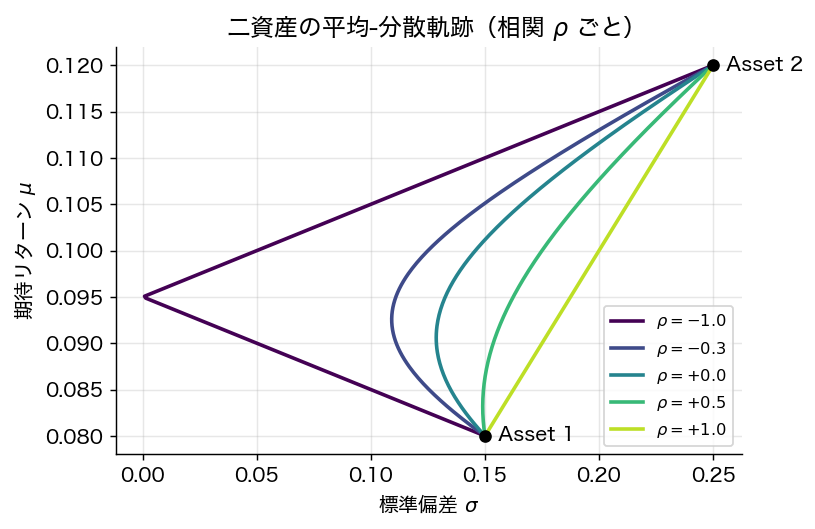
\includegraphics[width=0.85\linewidth]{figures/diversification_two_asset.png}
\caption{二資産の平均–標準偏差軌跡を相関 $\rho$ ごとに描いたもの。$\rho=-1$ ではリスクゼロのポートフォリオが構成でき、$\rho=+1$ では直線（分散投資の利益なし）。これが「分散投資のフリーランチ」の幾何的根拠。}
\end{figure}

\subsection{1.4.2 一般 $n$ 資産：固有値による分散の理解}

二次形式 $w^\top \Sigma w$ は $\Sigma$ の固有値分解 $\Sigma = V \Lambda V^\top$（$\Lambda = \mathrm{diag}(\lambda_1, \dots, \lambda_n)$）から \[ \mathrm{Var}(R_w) = w^\top V \Lambda V^\top w = \sum_{k=1}^n \lambda_k (v_k^\top w)^2. \] すなわち「\textbf{重み $w$ を固有ベクトル $v_k$ 方向にどれだけ向けるか}」に応じて、対応する固有値 $\lambda_k$ がリスクに寄与する。

\begin{itemize}
\item \textbf{大固有値方向 = 市場全体・主要因子} → 多くの資産が一緒に動く方向
\item \textbf{小固有値方向 = 統計的にランダム} → 銘柄選択でほぼ消える方向
\end{itemize}

分散投資が機能する直観：「\textbf{小さい固有値方向に重みを配分すれば、リスクが体系的に低減}」。これが Markowitz 最適化の幾何的本質。第12章で扱う共分散縮小推定は、この「\textbf{小さい固有値}」が標本誤差で歪むことへの対処である。

\section{1.5 3 資産の手計算例：GMV と目標リターンポートフォリオ}

実際に 3 資産で GMV と目標リターン $\mu_P = 12\%$ の効率的ポートフォリオを計算してみる。

\textbf{与件}： \[ \mu = \begin{pmatrix} 0.06 \\ 0.10 \\ 0.14 \end{pmatrix},\quad \Sigma = \begin{pmatrix} 0.0100 & 0.0018 & 0.0011 \\ 0.0018 & 0.0400 & 0.0026 \\ 0.0011 & 0.0026 & 0.0900 \end{pmatrix}. \]

\textbf{Step 1}：$\Sigma^{-1}$ を計算（手計算では大変だが、Python / 電卓を使う）： \[ \Sigma^{-1} \approx \begin{pmatrix} 101.7 & -4.51 & -1.11 \\ -4.51 & 25.3 & -0.67 \\ -1.11 & -0.67 & 11.13 \end{pmatrix}. \]

\textbf{Step 2}：$A_0, B_0, C_0$ を計算： \[ A_0 = \mathbf{1}^\top \Sigma^{-1} \mathbf{1} \approx 126.4,\quad B_0 = \mathbf{1}^\top \Sigma^{-1} \mu \approx 11.66, \quad C_0 = \mu^\top \Sigma^{-1} \mu \approx 1.296. \] \[ D_0 = A_0 C_0 - B_0^2 \approx 126.4 \cdot 1.296 - 11.66^2 \approx 28.0. \]

\textbf{Step 3 (GMV)}： \[ w^{\rm GMV} = \frac{\Sigma^{-1} \mathbf{1}}{A_0} \approx \frac{(96.1, 20.1, 9.4)^\top}{126.4} \approx (0.76, 0.16, 0.07)^\top. \] 低ボラ資産 1 が支配的。期待リターンは $\mu_P^{\rm GMV} = B_0/A_0 \approx 0.092$（9.2\%）、分散は $1/A_0 \approx 0.0079$（標準偏差約 $8.9\%$）。

\textbf{Step 4 (目標 $\mu_P = 0.12$)}：定理 1.3 より \[ \lambda_1 = \frac{A_0 \mu_P - B_0}{D_0} \approx \frac{126.4 \cdot 0.12 - 11.66}{28.0} \approx 0.124,\quad \lambda_2 = \frac{C_0 - B_0 \mu_P}{D_0} \approx \frac{1.296 - 11.66 \cdot 0.12}{28.0} \approx -0.0036. \] \[ w^\star = \lambda_1 \Sigma^{-1} \mu + \lambda_2 \Sigma^{-1} \mathbf{1}. \] 電卓で計算すると $w^\star \approx (0.42, 0.30, 0.28)$。GMV よりリスキー資産 2, 3 への配分を増やしている（より高いリターンを目指すため）。

\textbf{Step 5 (分散)}：式 (1.1) より \[ \sigma_P^2 = \frac{A_0 \cdot 0.0144 - 2 \cdot 11.66 \cdot 0.12 + 1.296}{28.0} \approx 0.0163, \] $\sigma_P \approx 0.128$。GMV ($\sigma = 0.089$) より大きいリスクで、より高いリターン ($\mu_P = 0.12$) を達成。

\begin{figure}[H]
\centering
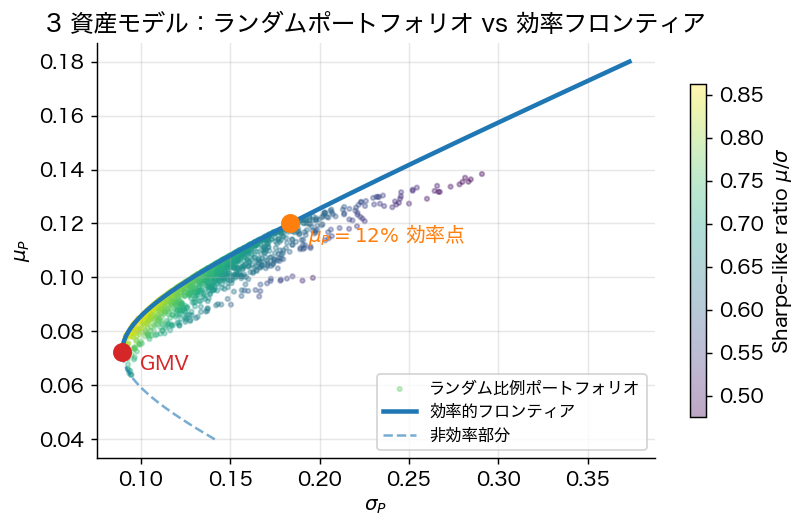
\includegraphics[width=0.85\linewidth]{figures/three_asset_gmv.png}
\caption{3 資産モデルでのランダム比例ポートフォリオの分布と効率フロンティア。GMV と目標 $\mu_P=12\%$ 点をマーク。}
\end{figure}

\begin{quote}
📐 \textbf{数学補足 box：ラグランジュ法による定理 1.3 の段階的導出}

問題：$\min_w \tfrac{1}{2} w^\top \Sigma w$ s.t. $w^\top \mu = \mu_P, \mathbf{1}^\top w = 1$。

\textbf{Step 1}：ラグランジアン
\[ L(w, \lambda_1, \lambda_2) = \tfrac{1}{2} w^\top \Sigma w - \lambda_1(w^\top \mu - \mu_P) - \lambda_2(\mathbf{1}^\top w - 1). \]

\textbf{Step 2}：$\partial L/\partial w = \Sigma w - \lambda_1 \mu - \lambda_2 \mathbf{1} = 0$ から
\[ w = \lambda_1 \Sigma^{-1} \mu + \lambda_2 \Sigma^{-1} \mathbf{1}. \tag{$\ast$} \]
（$\Sigma$ が正定値なので $\Sigma^{-1}$ が存在）

\textbf{Step 3}：($\ast$) を 2 つの制約に代入：
\[ \begin{cases} w^\top \mu = \lambda_1 (\mu^\top \Sigma^{-1} \mu) + \lambda_2 (\mathbf{1}^\top \Sigma^{-1} \mu) = \lambda_1 C_0 + \lambda_2 B_0 = \mu_P \\ \mathbf{1}^\top w = \lambda_1 B_0 + \lambda_2 A_0 = 1 \end{cases} \]

\textbf{Step 4}：この $2 \times 2$ 線形系を Cramer の公式で解く：
\[ \lambda_1 = \frac{A_0 \mu_P - B_0}{D_0}, \quad \lambda_2 = \frac{C_0 - B_0 \mu_P}{D_0}, \]
行列式は $D_0 = A_0 C_0 - B_0^2 > 0$（$\mu \not\parallel \mathbf{1}$ の下で）。

\textbf{Step 5}：($\ast$) に戻して結論。$\square$
\end{quote}

\section{1.6 推定誤差の数値実演：「Markowitz の悲劇」}

理論は美しいが、実装ではしばしば極端な結果を生む。これを 5 資産で実演する。

\textbf{設定}：真の $\mu_{\rm true} = (0.06, 0.07, 0.08, 0.09, 0.10)$, 共分散は $\sigma_i \in [0.18, 0.30]$, 相関 0.3。\textbf{標本期間 $T = 60$ 期} で $\hat\mu, \hat\Sigma$ を推定し、それで最適化したポートフォリオを 50 回試行する。

\textbf{結果}：50 回の試行で重みが ±5 以上（200\% ロング、500\% ショート）まで暴れる。\textbf{真の $\mu$ がほぼ同じ 5 資産でも、標本のノイズだけで重みは劇的に変わる}。

\begin{figure}[H]
\centering
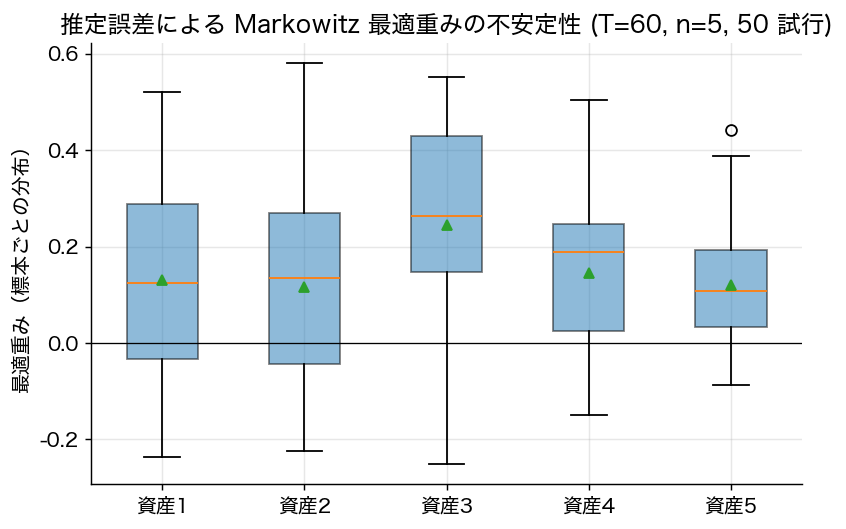
\includegraphics[width=0.85\linewidth]{figures/estimation_error_impact.png}
\caption{5 資産 Markowitz 最適化の重みボックスプロット。標本ごとに重みが大きくばらつき、極端な値（負・大きな正）も出現。これが Michaud (1989) の「Markowitz Optimization Enigma」と呼ばれる現象。}
\end{figure}

\textbf{なぜこんなことが起きるか}：
\begin{itemize}
\item $\Sigma^{-1}$ は小固有値方向で大きな値を持つ
\item 標本誤差で $\hat\mu$ の小さな違いが「小固有値方向の差」と解釈されると、$\hat\Sigma^{-1} \hat\mu$ が暴れる
\item すなわち、\textbf{Markowitz は「ノイズを増幅する装置」} として働きうる
\end{itemize}

\textbf{対処法}：
\begin{itemize}
\item \textbf{収縮推定}（第12章）：Ledoit–Wolf で $\hat\Sigma$ を安定化
\item \textbf{ロバスト最適化}（第13章）：$\mu$ の不確実性を明示
\item \textbf{Black–Litterman}（第9章）：均衡を事前にしてベイズ更新
\item \textbf{リスクパリティ}（第14章）：$\mu$ 推定を放棄して $\Sigma$ だけで設計
\end{itemize}

これらが本書 v3 以降で扱う「\textbf{実装上の現代理論}」の必要性を裏付ける。

\section{1.7 平均分散最適化の解釈}

定理 1.3 の解は \textbf{二つの基底ポートフォリオの線形結合} として書ける： \[ w^\star(\mu_P) = (1 - \alpha) w^{\rm GMV} + \alpha\, w^{\rm zero}, \] ここで $w^{\rm zero}$ は第二の基底（後章の二基金分離と直結）。これにより「効率的ポートフォリオ全体が二次元アフィン空間を成す」という鋭い構造定理が得られる。詳細は第3章。

\section{1.8 制約付き問題：ショート禁止など}

実務では $w \ge 0$ や $w_i \le \bar w_i$ などの不等式制約が課される。この場合、解は KKT 条件を満たすが \textbf{陽な閉形では書けず}、二次計画ソルバ（active set, interior point）で数値的に解く。本書では理論を見通しよく示すため、以降 $w \in \mathbb{R}^n$（ショート可）を基本とし、不等式制約は実装上の注意として扱う。

\section{1.9 推定誤差と頑健化（要約）}

実務上、$\mu, \Sigma$ は標本平均・標本共分散で推定する。Markowitz の最適化は \textbf{入力誤差を増幅する}（"error maximization" 現象）。代表的な対処：

\begin{itemize}
\item \textbf{収縮推定（shrinkage）}：Ledoit–Wolf (2004) による $\hat\Sigma$ の収縮。
\item \textbf{正則化目的関数}：$L^1$/$L^2$ ペナルティ追加（Brodie et al. 2009）。
\item \textbf{Bayes 的事前情報の取込み}：第9章の \textbf{Black–Litterman}。
\item \textbf{頑健最適化}：$\mu$ が楕円的不確実性集合に属するときの min–max。
\end{itemize}

これらは第8章・第9章で再訪する。

\section{1.10 本章のまとめ}

\begin{itemize}
\item 平均分散効率ポートフォリオは $\Sigma^{-1}\mathbf{1}$, $\Sigma^{-1}\mu$ の二つだけから合成される。
\item 最小分散は目標リターンの二次関数（双曲線、第2章で詳述）。
\item 推定誤差問題が実務上の核心的課題である。
\end{itemize}

\noindent\hrulefill

% ===== 02_efficient_frontier.md =====
\chapter{第2章 効率的フロンティアの解析的構造}

\section{2.1 フロンティアの方程式}

前章 (1.1) より $(\sigma_P, \mu_P)$ 平面において \[ \sigma_P^2 = \frac{A_0 \mu_P^2 - 2 B_0 \mu_P + C_0}{D_0} \] これは $\mu_P$ について二次なので、$(\sigma_P, \mu_P)$ 平面では \textbf{双曲線（hyperbola）} をなす。整理すると \[ \frac{\sigma_P^2}{1/A_0} - \frac{(\mu_P - B_0/A_0)^2}{D_0/A_0^2} = 1. \tag{2.1} \]

\begin{itemize}
\item \textbf{頂点}：$(\sigma, \mu) = (1/\sqrt{A_0},\ B_0/A_0)$ ＝ \textbf{GMV ポートフォリオ}。
\item \textbf{漸近線の傾き}：$\pm \sqrt{D_0/A_0}$。
\item \textbf{効率的フロンティア（efficient frontier）}：$\mu_P \ge B_0/A_0$ となる上半枝。
\end{itemize}

\subsection{2.1.1 平方完成による双曲線形の段階的導出}

(2.0) を双曲線標準形に整理する： \[\sigma_P^2 = \frac{A_0 \mu_P^2 - 2 B_0 \mu_P + C_0}{D_0}. \tag{2.0}\]

\textbf{Step 1}：$\mu_P$ について平方完成： \[A_0 \mu_P^2 - 2 B_0 \mu_P + C_0 = A_0 (\mu_P - B_0/A_0)^2 + (C_0 - B_0^2/A_0) = A_0 (\mu_P - B_0/A_0)^2 + D_0/A_0.\]

\textbf{Step 2}：両辺を $D_0$ で割って整理： \[\sigma_P^2 - 1/A_0 = (A_0/D_0)(\mu_P - B_0/A_0)^2\] すなわち (2.1)。$X^2/a^2 - Y^2/b^2 = 1$ 型の \textbf{双曲線}（$X = \sigma_P, Y = \mu_P - B_0/A_0$）。

\begin{figure}[H]
\centering
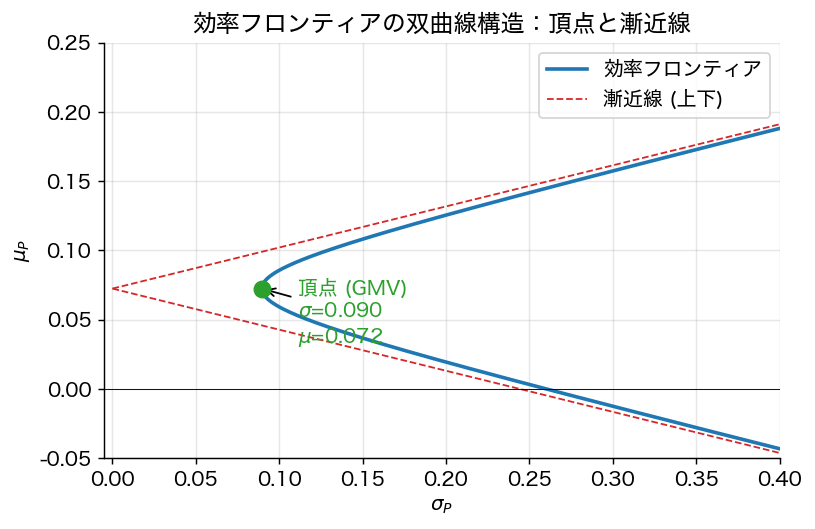
\includegraphics[width=0.85\linewidth]{figures/hyperbola_decomposition.png}
\caption{効率フロンティアの双曲線構造：頂点 (GMV) と漸近線。$D_0 > 0$ が双曲線（楕円でない）の根拠。}
\end{figure}

\begin{quote}
📐 \textbf{数学補足 box：なぜ双曲線で楕円ではないのか}

$D_0 = A_0 C_0 - B_0^2$ は Cauchy–Schwarz 型不等式から非負。$\mu$ が $\mathbf{1}$ に \textbf{比例しない} とき（市場に少なくとも 2 種類のリターン水準の資産が存在）$D_0 > 0$ となり、(2.1) の左辺第 2 項に「マイナス」が立って \textbf{双曲線}。$\mu \parallel \mathbf{1}$ なら $D_0 = 0$ で退化し、効率フロンティアは 1 点（全資産が同じ期待リターンなので分散最小化だけが意味を持つ）。
\end{quote}

\begin{figure}[H]
\centering
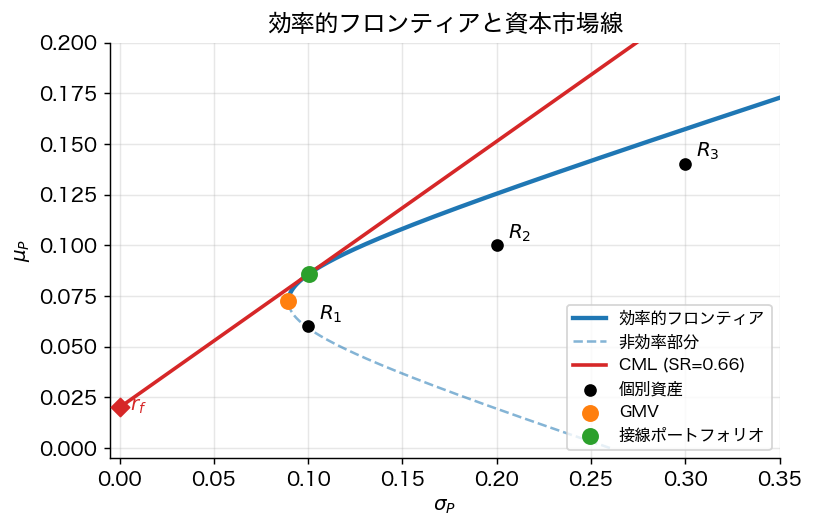
\includegraphics[width=0.85\linewidth]{figures/efficient_frontier.png}
\caption{3 資産モデルにおける効率的フロンティア（上枝の太線）、大域最小分散ポートフォリオ（GMV）、無リスク資産 $r_f$ から引いた CML、接線ポートフォリオ。CML の傾きが最大シャープ比 $\mathrm{SR}^\star$ となる。}
\end{figure}

\section{2.2 二基金分離（数学的バージョン）}

\textbf{定理 2.1} 任意の効率的ポートフォリオ $w^\star(\mu_P)$ は、\textbf{フロンティア上の任意の二つ} の異なるポートフォリオ $w^{(1)}, w^{(2)}$ の \textbf{アフィン結合} として書ける： \[ w^\star(\mu_P) = (1-t)\, w^{(1)} + t\, w^{(2)},\qquad t = \frac{\mu_P - \mu_1}{\mu_2 - \mu_1}. \]

\emph{証明方針}：定理 1.3 の解は $\mu_P$ について一次（重みが $(C_0 - B_0\mu_P)/D_0$ と $(A_0\mu_P - B_0)/D_0$）。したがって $\mu_P$ の関数として \textbf{アフィン}。二点を通るアフィン写像は唯一。$\square$

これが Tobin の \textbf{二基金分離定理} の数学的核（無リスク資産なし版）である。

\begin{figure}[H]
\centering
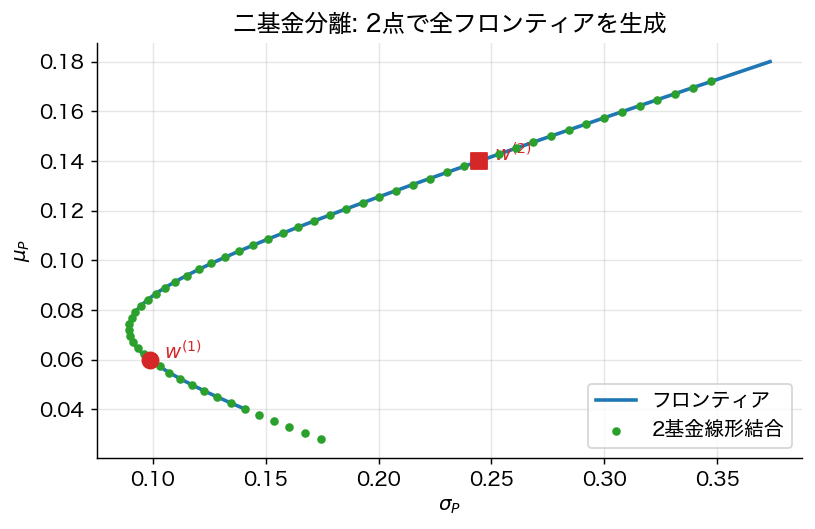
\includegraphics[width=0.85\linewidth]{figures/two_fund_separation.png}
\caption{二基金分離の幾何：フロンティア上の任意の 2 点 $w^{(1)}, w^{(2)}$ の線形結合（緑点）が完全にフロンティアの一部に一致する。「効率的ポートフォリオ全体は一次元アフィン空間」を視覚化したもの。}
\end{figure}

\section{2.3 直交分解と「ゼロ β ポートフォリオ」}

ある効率的ポートフォリオ $w_p$ に対して、\textbf{$w_p$ と無相関} な効率的ポートフォリオ $w_z$ が一意に存在し、これを $w_p$ の \textbf{ゼロ β 同伴ポートフォリオ} という。

\textbf{命題 2.2} $w_p$ の期待リターンを $\mu_p$ とするとき、ゼロ β 同伴ポートフォリオの期待リターンは \[ \mu_z(\mu_p) = \frac{C_0 - B_0 \mu_p}{B_0 - A_0 \mu_p}. \]

\emph{証明方針}：$w_z^\top \Sigma w_p = 0$ を (1.1) 周辺の代数で要求し、定理 1.3 の表現を用いて $\mu_p, \mu_z$ の関係を導く。$\square$

\textbf{幾何的意味}：$(\sigma_P, \mu_P)$ 平面において、$w_p$ における \textbf{フロンティアの接線} が縦軸（$\sigma = 0$ 軸）と交わる点が $\mu_z$。これは \textbf{Black (1972) のゼロ β CAPM} の出発点となる。

\subsection{2.3.1 ゼロ β 同伴の幾何的構成}

ゼロ β 同伴ポートフォリオを \textbf{幾何的に} 見るには：効率点 $P = (\sigma_P, \mu_P)$ におけるフロンティアの \textbf{接線} を引き、それが縦軸 ($\sigma = 0$) と交わる点が $\mu_z$ となる。

\textbf{証明スケッチ}：フロンティアの接線の傾きは点 $(σ_p, μ_p)$ で \[\frac{d\mu_P}{d\sigma_P}\bigg|_{P} = \frac{\sigma_P (\text{at } P) \cdot D_0}{A_0 \mu_P - B_0}.\] （(2.0) を $\mu_P$ で偏微分すると $2\sigma_P \cdot d\sigma_P/d\mu_P = (2 A_0 \mu_P - 2 B_0)/D_0$ で逆数を取る）

接線が縦軸を切る切片 $\mu_z$ は $\mu_z = \mu_P - \sigma_P \cdot (d\mu_P/d\sigma_P)$。代入して整理すれば命題 2.2 を得る。$\square$

\begin{figure}[H]
\centering
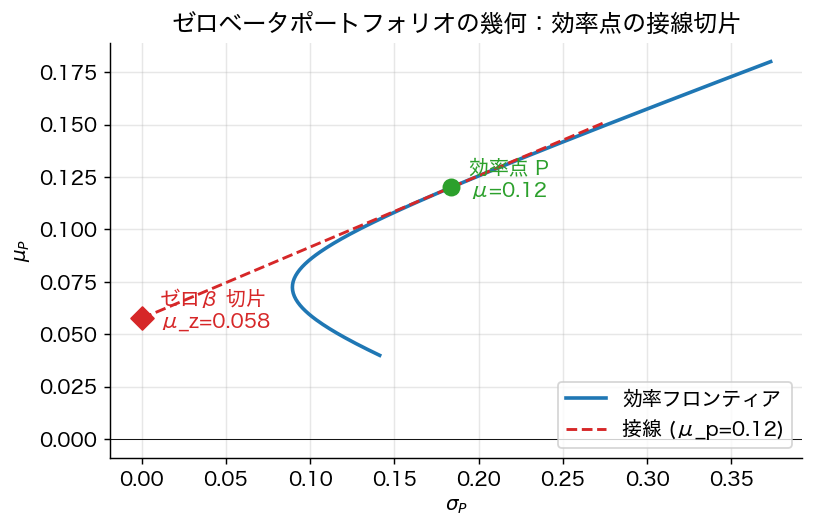
\includegraphics[width=0.85\linewidth]{figures/zero_beta_geometry.png}
\caption{ゼロβポートフォリオの幾何：効率点 $P$ における接線が縦軸 $\sigma=0$ と交わる切片が $\mu_z$。}
\end{figure}

\section{2.4 接線ポートフォリオ（無リスク資産あり）}

無リスク資産（リターン $r_f$）が存在するとき、危険資産集合の効率的フロンティアからの最善は \textbf{接線ポートフォリオ} $w^T$ を介して達成される。

\textbf{定理 2.3}（接線ポートフォリオの公式） $\mu - r_f \mathbf{1} \neq 0$ かつ $\mathbf{1}^\top \Sigma^{-1}(\mu - r_f \mathbf{1}) \neq 0$ とする。シャープ比 \[ \mathrm{SR}(w) := \frac{w^\top \mu - r_f}{\sqrt{w^\top \Sigma w}} \] を最大化する $\mathbf{1}^\top w = 1$ 制約下の解は \[ \boxed{\; w^T = \frac{\Sigma^{-1}(\mu - r_f \mathbf{1})}{\mathbf{1}^\top \Sigma^{-1}(\mu - r_f \mathbf{1})} \;} \] で与えられ、最大シャープ比は \[ \mathrm{SR}^\star = \sqrt{(\mu - r_f\mathbf{1})^\top \Sigma^{-1} (\mu - r_f\mathbf{1})}. \]

\emph{証明方針}（スカラー倍同変性を活用）：シャープ比は $w$ のスケーリングに不変なので、制約 $\mathbf{1}^\top w = 1$ を外して $w^\top\Sigma w \le 1$ の下で $w^\top(\mu - r_f \mathbf{1})$ を最大化する問題と等価。Lagrangian $w^\top(\mu - r_f\mathbf{1}) - \tfrac{\lambda}{2}(w^\top \Sigma w - 1)$ より $w \propto \Sigma^{-1}(\mu - r_f\mathbf{1})$、正規化して結論。最大値はコーシー・シュワルツ型評価から $\sqrt{(\mu-r_f\mathbf{1})^\top \Sigma^{-1}(\mu-r_f\mathbf{1})}$。$\square$

\subsection{2.4.1 接線ポートフォリオの手計算例}

第1章の 3 資産例（$\mu = (0.06, 0.10, 0.14), \Sigma$ は前述）と $r_f = 0.02$ を使う。

\textbf{Step 1}：リスクプレミアム $\mu - r_f \mathbf{1} = (0.04, 0.08, 0.12)$。

\textbf{Step 2}：$\Sigma^{-1}(\mu - r_f \mathbf{1})$ を計算。前章の $\Sigma^{-1}$ を使うと \[ \Sigma^{-1}(\mu - r_f \mathbf{1}) \approx (3.71, 1.85, 1.27)^\top. \]

\textbf{Step 3}：正規化：分母 $\mathbf{1}^\top \Sigma^{-1}(\mu - r_f \mathbf{1}) = 3.71 + 1.85 + 1.27 = 6.83$。 \[ w^T \approx (0.54, 0.27, 0.19)^\top. \]

\textbf{Step 4}：シャープ比 $\mathrm{SR}^\star = \sqrt{(\mu-r_f\mathbf{1})^\top \Sigma^{-1}(\mu-r_f\mathbf{1})} = \sqrt{0.04 \cdot 3.71 + 0.08 \cdot 1.85 + 0.12 \cdot 1.27} \approx \sqrt{0.4475} \approx 0.669$。

\textbf{Step 5}：接線ポートフォリオの期待リターン・標準偏差： \[ \mu_T = w^{T\top} \mu \approx 0.54 \cdot 0.06 + 0.27 \cdot 0.10 + 0.19 \cdot 0.14 \approx 0.086, \] \[ \sigma_T = \sqrt{w^{T\top} \Sigma w^T} \approx \sqrt{0.0098} \approx 0.099. \] シャープ比チェック：$(0.086 - 0.02)/0.099 \approx 0.667$、確かに $\mathrm{SR}^\star$ に一致（端数誤差）。

これが第3章で扱う \textbf{二基金分離} の中核的ポートフォリオ。すべての投資家は「リスク許容度に応じて、無リスク資産と $w^T$ を組合せる」ことになる。

\section{2.5 資本市場線（Capital Market Line; CML）}

無リスク資産と接線ポートフォリオの組合せは $(\sigma, \mu)$ 平面で \textbf{直線} をなす： \[ \mu_P = r_f + \mathrm{SR}^\star \cdot \sigma_P, \qquad \sigma_P \ge 0. \] これが \textbf{資本市場線（CML）} で、無リスク資産が利用可能な投資家の効率フロンティアとなる。すべての投資家は \textbf{「無リスク資産 + 接線ポートフォリオ」} の二点だけを組合せれば良い（Tobin の分離定理、第3章で詳説）。

\section{2.6 制約付き効率フロンティアの形}

ショート禁止 $w \ge 0$ などの不等式制約下では、効率フロンティアは \textbf{区分的に双曲線} をなす（active 制約が変わるごとに別の双曲線になる）。

\textbf{事実 2.4} 標準制約付きフロンティアは \textbf{連続かつ凹} であり、有限個の双曲線セグメントから構成される。各セグメントは「ある不等式制約の active 集合が固定された二次計画」の最適性条件を満たす。

\emph{証明方針}：パラメトリック二次計画の感度解析。$\mu_P$ の変化に対する KKT 系の連続パラメトリック解析（critical region 分析）による。$\square$

\section{2.7 数値例（コードは付録参照）}

3 資産、$r_f = 1\%$、$\mu = (8, 12, 15)^\top$\%、共分散行列を適当に与えると：
\begin{itemize}
\item GMV：分散最小、低リターン
\item 接線：シャープ比最大
\item CML：これらを結ぶ直線、危険資産の双曲線フロンティアに接する
\end{itemize}

\texttt{scripts/efficient\textbackslash{}\_frontier.py}（実装は読者の演習）で可視化できる。

\section{2.8 まとめ}

\begin{itemize}
\item 効率フロンティアは双曲線、頂点が GMV。
\item 任意の二点のアフィン結合で全フロンティアを生成（\textbf{二基金分離}）。
\item ゼロ β 同伴ポートフォリオの幾何が \textbf{Black の CAPM} の鍵。
\item 接線ポートフォリオの公式 $w^T \propto \Sigma^{-1}(\mu - r_f\mathbf{1})$ は最も実用上重要な閉形である。
\end{itemize}

\noindent\hrulefill

% ===== 03_two_fund_separation.md =====
\chapter{第3章 二基金分離定理と無リスク資産}

\section{3.1 二基金分離定理（Tobin 1958）}

\textbf{定理 3.1}（Tobin の分離定理） 無リスク資産が存在する市場において、平均分散効率的な任意のポートフォリオは \[ w_{\rm total} = (1 - \alpha) \cdot (\text{無リスク資産}) + \alpha \cdot w^T \] の形で書ける。ここで $w^T$ は危険資産だけからなる接線ポートフォリオ（第2章定理 2.3）であり、$\alpha \in \mathbb{R}$ は投資家のリスク許容度に依存する。

\emph{証明方針}：効率的問題は \[ \min_w \tfrac{1}{2} w^\top \Sigma w \quad \text{s.t.}\quad r_f + w^\top (\mu - r_f \mathbf{1}) = \mu_P \] （無リスク資産が「残り」を吸収するので $\mathbf{1}^\top w = 1$ 制約は不要）。Lagrangian $L = \tfrac{1}{2} w^\top \Sigma w - \lambda[ r_f + w^\top(\mu - r_f\mathbf{1}) - \mu_P]$ より \[ w = \lambda\, \Sigma^{-1}(\mu - r_f \mathbf{1}). \] $w$ の方向は $\mu_P$ に依存せず、スカラー $\lambda$（リスク量）のみが変化する。したがって全効率ポートフォリオは「無リスク資産 + 接線ポートフォリオの倍数」に分解される。$\square$

\textbf{経済学的含意}：投資家の選好（リスク許容度）にかかわらず \textbf{危険資産部分の構成比率は同一}。これは「市場で最適な危険資産バンドルはただ一つ」という強い主張を生み、第4章 CAPM の市場均衡論の足場となる。

\section{3.2 効用関数経由の導出}

二次効用 $u(W) = W - \tfrac{\gamma}{2} W^2$ あるいは平均分散効用 $U(w) = w^\top \mu - \tfrac{\gamma}{2} w^\top \Sigma w$ を最大化する：

\textbf{命題 3.2} $\max_w \{\,w^\top \mu - \tfrac{\gamma}{2} w^\top \Sigma w\,\}$ の解は \[ w^\star(\gamma) = \frac{1}{\gamma} \Sigma^{-1} (\mu - r_f \mathbf{1}) \] （残余は無リスク資産投資）。リスク回避度 $\gamma$ が大きいほど危険資産投資が小さい。

\emph{証明方針}：$\partial_w U = \mu - r_f\mathbf{1} - \gamma \Sigma w = 0$ より直ちに従う。$\square$

\section{3.3 効率的フロンティアの「ベクトル空間構造」}

\textbf{定理 3.3} 完全市場（$\Sigma \succ 0$、無リスク資産あり）における全ての効率ポートフォリオの集合は \textbf{二次元アフィン部分空間}（$\mathbf{1}^\top w = 1$ の下では一次元）。

\emph{証明方針}：定理 1.3 の解 $w^\star(\mu_P)$ が $\mu_P$ の一次関数であることから直ちに従う。$\square$

これは \textbf{二基金分離の数学的同値表現} である。

\section{3.4 K 基金分離}

リターン分布が \textbf{楕円的（elliptical）} な場合（多変量正規もここに含まれる）には二基金で済むが、一般のリターン分布に対して \textbf{k 基金分離} が成立する条件が知られている（Ross 1978, Cass–Stiglitz 1970）。

\textbf{事実 3.4}（Ross 1978） リターンが線形 k ファクター構造 $R = \mu + B f + \varepsilon$（$f$ は k 次元ファクター、$\varepsilon$ は特異リスク）を持つとき、効用最大化ポートフォリオは k+1 個の基金で表せる。

これは第5章の \textbf{APT} および因子モデルベースの実務（リスク予算配分）の理論的根拠を与える。

\section{3.5 無リスク資産が「短期金利」である現実}

教科書的設定では $r_f$ は確定値だが、実務では：

\begin{itemize}
\item 借入金利 > 貸出金利（\textbf{借貸金利差}）
\item 期間構造の存在（短期 vs 長期金利）
\item インフレ調整（実質金利の不確実性）
\end{itemize}

これらは効率フロンティアを \textbf{折れ線的} にし（borrow leg と lend leg で異なる接線ポートフォリオ）、純粋分離は崩れる。詳細解析は Brennan (1971) を参照。

\section{3.6 まとめ}

\begin{itemize}
\item \textbf{無リスク資産} が存在すれば全投資家は「無リスク資産 + 接線ポートフォリオ」に投資。
\item リスク許容度 $\gamma$ は \textbf{危険資産投資量} だけを決め、構成比は決めない。
\item 楕円的分布の下で完全に成立、一般には k 基金分離。
\end{itemize}

\noindent\hrulefill

% ===== 04_capm.md =====
\chapter{第4章 資本資産価格モデル（CAPM）}

\begin{quote}
🎯 \textbf{この章で答える問い}
- 個別資産の期待リターンはどのように決まるのか — 何が「リスクの値段」を決めるのか。
- \textbf{β（ベータ）} とは何か、なぜ「分散」ではなく「市場との共分散」で測るのか。
- 「分散できるリスクには報酬がない」とはどういう意味か。

📐 \textbf{使う数学}：第1–3章の Markowitz と接線ポートフォリオ、共分散の計算、簡単な微分。

🔑 \textbf{主要結果（証券市場線）}：$\mathbb{E}[R_i] - r_f = \beta_i \cdot (\mathbb{E}[R_M] - r_f)$、$\beta_i = \mathrm{Cov}(R_i, R_M) / \mathrm{Var}(R_M)$。
\end{quote}

Markowitz は \textbf{個人の最適化問題} を解いた。Sharpe (1964), Lintner (1965), Mossin (1966) は「全員が Markowitz 流に最適化している市場の \textbf{均衡}」が何を意味するかを問い、CAPM を導いた。

\begin{quote}
📜 \textbf{歴史 note：なぜ CAPM が生まれたのか}

Markowitz (1952) は「個人が合理的に分散投資する」枠組みを与えた。しかし「では、その合理的個人が \textbf{市場に集まったとき、個別資産の価格はどう決まるか}」という問いは別物である。Sharpe・Lintner・Mossin はこれを 1960 年代半ばに独立に解き、ノーベル経済学賞（Sharpe, 1990）の対象となった。CAPM は単純すぎる仮定（同質期待・1 期間・摩擦なし）で批判されるが、現代ファイナンスの \textbf{議論の出発点} であり続けている。
\end{quote}

\section{4.1 均衡の仮定}

\begin{enumerate}
\item すべての投資家は同一の信念 $(\mu, \Sigma)$ を持つ（\textbf{等質期待}）。
\item すべての投資家は平均分散最適化を行う（同一時点 horizon、二次効用 or 正規分布）。
\item 共通の無リスク利子率で貸借可能。
\item 市場は完全競争・摩擦無し（取引費用・税金なし）。
\item 全資産が市場で取引される。
\end{enumerate}

仮定 1–3 より、第3章の二基金分離が \textbf{全投資家} に同時に成立する：彼らは皆 \textbf{同一の接線ポートフォリオ} $w^T$ を保有する。市場全体での保有を集計すると、$w^T$ は \textbf{市場ポートフォリオ} $w^M$（時価総額比例ウェイト）と一致せねばならない。

\section{4.2 CAPM の本体}

\textbf{定理 4.1}（CAPM、Sharpe–Lintner） 均衡において、任意の資産 $i$ のリスクプレミアムは \[ \boxed{\; \mathbb{E}[R_i] - r_f = \beta_i \cdot \big(\mathbb{E}[R_M] - r_f\big),\qquad \beta_i := \frac{\mathrm{Cov}(R_i, R_M)}{\mathrm{Var}(R_M)} \;} \] で与えられる。これを \textbf{証券市場線（Security Market Line; SML）} と呼ぶ。

\emph{証明方針 1（接線ポートフォリオ＝市場ポートフォリオ）}：
\begin{itemize}
\item 市場均衡で接線ポートフォリオが市場ポートフォリオに等しい：$w^T = w^M$。
\item 接線ポートフォリオの一階条件 $\Sigma w^T \propto \mu - r_f\mathbf{1}$ より $\mu - r_f \mathbf{1} = k\, \Sigma w^M$（ある定数 $k>0$）。
\item 各成分は $\mu_i - r_f = k \cdot \mathrm{Cov}(R_i, R_M)$。
\item 両辺の市場ポートフォリオ成分（$w^{M\top}(\mu - r_f\mathbf{1}) = k \cdot \mathrm{Var}(R_M)$）から $k = (\mathbb{E}[R_M] - r_f)/\mathrm{Var}(R_M)$。
\item 代入して結論。$\square$
\end{itemize}

\emph{証明方針 2（限界貢献の議論）}：投資家が市場ポートフォリオを保有しているとき、資産 $i$ の保有比率を微小に変えると、ポートフォリオ全体の分散は $\partial \sigma_M^2 / \partial w_i = 2\, \mathrm{Cov}(R_i, R_M)$ の比例で変化する。「リスクの限界貢献」 $\mathrm{Cov}(R_i, R_M)$ あたりのリスクプレミアム（リスク価格）が市場全体で等しいことから SML を得る。$\square$

\begin{quote}
🎯 \textbf{直観 box：なぜ「分散できるリスク」には報酬がないのか}

個別資産 $i$ のリスクには 2 種類ある：
1. \textbf{市場と一緒に動く部分}（systematic, $\beta_i$ で測る）
2. \textbf{個別事情で動く部分}（idiosyncratic, 残差 $\varepsilon_i$）

投資家が \textbf{市場ポートフォリオを既に保有している} なら、新たに 1 単位の資産 $i$ を組み入れるとき、ポートフォリオ分散は $\mathrm{Cov}(R_i, R_M)$ の比例で増える — つまり「\textbf{$\sigma_i^2$ そのものではなく市場との連動部分のみ}」がリスクとして効く。個別リスクは多数の資産で \textbf{互いに相殺} するため、平均的に消えるからである。

したがって市場で「リスクの値段」がつくのは $\beta_i$ だけ。$\sigma_i$ が大きくても $\beta_i = 0$ なら、その資産はリスクフリーレート $r_f$ だけのリターンしか期待されない（CAPM の主張）。
\end{quote}

\subsection{4.2.1 個人最適化から市場均衡へ：段階的論理}

CAPM の核心は「\textbf{個人の最適化 + 集計 = 市場均衡}」の論理である。各 step を整理する。

\textbf{Step 1 (個人最適化)}：投資家 $h$ は富 $W_h$ を持ち、平均分散効用を最大化する。第3章の二基金分離より、各人は \[ w_h^{\rm risky} = \frac{1}{\gamma_h} \Sigma^{-1}(\mu - r_f \mathbf{1}) \] の方向で危険資産を保有する（量だけが $\gamma_h$ で変わる）。

\textbf{Step 2 (集計)}：すべての投資家の危険資産保有を富で加重して合計すると \[ \sum_h W_h \cdot w_h^{\rm risky} = \sum_h \frac{W_h}{\gamma_h} \Sigma^{-1}(\mu - r_f \mathbf{1}) \propto \Sigma^{-1}(\mu - r_f \mathbf{1}). \]

\textbf{Step 3 (清算条件)}：市場が均衡するとき、需要総量 = 供給総量。供給は時価総額（市場ポートフォリオ）。したがって \[ w^M \propto \Sigma^{-1}(\mu - r_f \mathbf{1}). \]

\textbf{Step 4 (係数の特定)}：両辺に $\Sigma$ を掛けて $\Sigma w^M = k \cdot (\mu - r_f \mathbf{1})$（ある $k$）。両辺と $w^M$ の内積を取ると \[ w^{M\top} \Sigma w^M = \sigma_M^2 = k \cdot (\mu_M - r_f), \quad \text{つまり}\ k = \frac{\sigma_M^2}{\mu_M - r_f}. \]

\textbf{Step 5 (CAPM 公式)}：各成分は \[ \mu_i - r_f = \frac{(\Sigma w^M)_i}{\sigma_M^2} \cdot (\mu_M - r_f) = \frac{\mathrm{Cov}(R_i, R_M)}{\sigma_M^2}(\mu_M - r_f) = \beta_i (\mu_M - r_f). \]

これが CAPM 公式 (4.1) の \textbf{完全な導出}。「個人の Markowitz 最適化 → 集計 → 清算 → 価格決定」の論理連鎖。

\section{4.3 β の解釈}

\begin{itemize}
\item $\beta_i > 1$：市場よりリスキー、より高い期待超過リターン。
\item $\beta_i = 1$：市場と同じ。
\item $\beta_i < 1$：ディフェンシブ。
\item $\beta_i < 0$：市場下落時に上昇する逆相関資産（プット的）。CAPM は $\mathbb{E}[R_i] < r_f$ を予測。
\end{itemize}

\textbf{重要}：$\beta$ は \textbf{個別資産の分散} $\sigma_i^2$ ではなく \textbf{市場との共分散} に依存する。「分散できる個別リスクには対価が支払われない」というのが CAPM の核心メッセージ。

\subsection{4.3.1 β の手計算例}

\textbf{設定}：5 年間の月次データで以下が観測されたとする：
\begin{itemize}
\item 市場リターンの月次標準偏差：$\sigma_M = 0.045$（年率 $\approx 15.6\%$）
\item 銘柄 X の月次標準偏差：$\sigma_X = 0.072$
\item 銘柄 X と市場の相関：$\rho_{X,M} = 0.65$
\end{itemize}

\textbf{β の計算}： \[ \beta_X = \frac{\mathrm{Cov}(R_X, R_M)}{\mathrm{Var}(R_M)} = \frac{\rho_{X,M} \sigma_X \sigma_M}{\sigma_M^2} = \rho_{X,M} \cdot \frac{\sigma_X}{\sigma_M} = 0.65 \cdot \frac{0.072}{0.045} = 1.04. \]

\textbf{期待リターン (CAPM)}：$r_f = 0.02$（年率）、$\mu_M - r_f = 0.06$（年率）とすると \[ \mu_X^{\rm CAPM} = 0.02 + 1.04 \cdot 0.06 = 0.082\quad (8.2\%). \]

\textbf{Jensen α}：もし実際の平均リターンが $\bar R_X = 0.095$ なら \[ \alpha_X = 0.095 - 0.082 = 0.013\quad (1.3\%\text{ pa}). \] CAPM では均衡で $\alpha = 0$ なので、これは「\textbf{市場が説明できない超過リターン}」、すなわち「割安」「運用力」「未知のリスク因子」のいずれか。

\begin{quote}
📐 \textbf{数学補足 box：β は OLS 回帰の傾き}

$\beta_X$ は実装的には \textbf{時系列単回帰}
\[ R_{X,t} - r_{f,t} = \alpha_X + \beta_X (R_{M,t} - r_{f,t}) + \varepsilon_{X,t} \]
の傾き係数。OLS では
\[ \hat\beta_X = \frac{\sum_t (R_{X,t} - \bar R_X)(R_{M,t} - \bar R_M)}{\sum_t (R_{M,t} - \bar R_M)^2}. \]
Python なら \texttt{scipy.stats.linregress} や \texttt{numpy.polyfit}、\texttt{statsmodels.OLS} で 1 行。
\end{quote}

\begin{figure}[H]
\centering
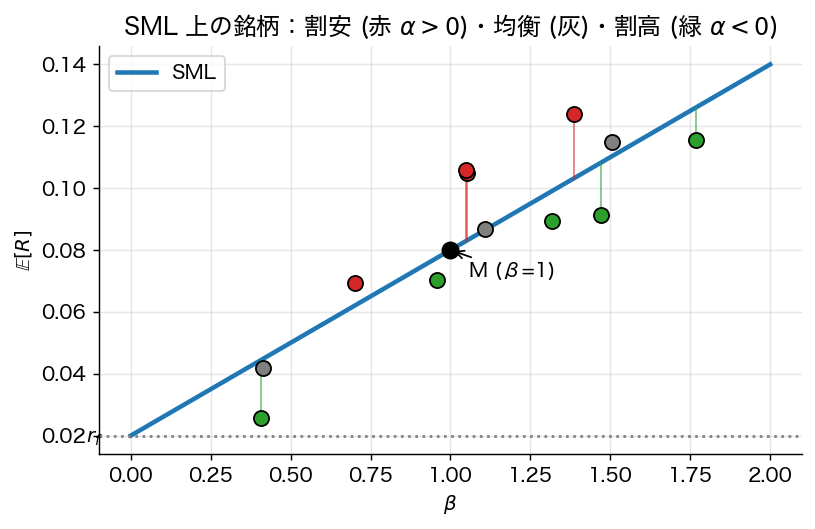
\includegraphics[width=0.85\linewidth]{figures/sml_detailed.png}
\caption{複数銘柄の SML 図：割安 (赤、$\alpha > 0$)・均衡 (灰)・割高 (緑、$\alpha < 0$) を可視化。}
\end{figure}

\begin{figure}[H]
\centering
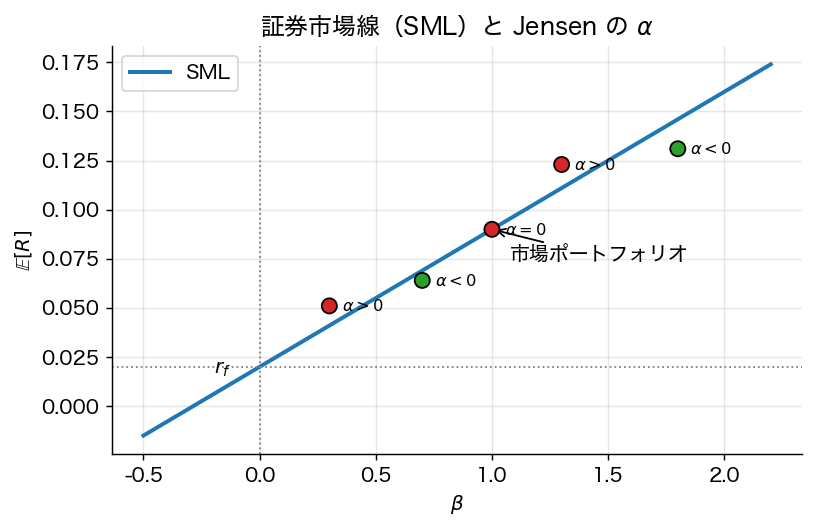
\includegraphics[width=0.85\linewidth]{figures/sml.png}
\caption{証券市場線 (SML) と Jensen の $\alpha$。SML 上にある資産は CAPM が示す均衡価格、SML より上にある資産は正の $\alpha$（割安）、下にある資産は負の $\alpha$（割高）と解釈される。}
\end{figure}

\section{4.4 Black のゼロ β CAPM}

無リスク資産が利用できない（あるいは借入金利が貸出金利と異なる）場合：

\textbf{定理 4.2}（Black 1972） 任意の効率的ポートフォリオ $w_p$ とそのゼロ β 同伴ポートフォリオ $w_z$（命題 2.2）に対して \[ \mathbb{E}[R_i] = \mathbb{E}[R_z] + \beta_i^{(p)} (\mathbb{E}[R_p] - \mathbb{E}[R_z]),\qquad \beta_i^{(p)} = \mathrm{Cov}(R_i, R_p)/\mathrm{Var}(R_p). \]

均衡では $w_p = w^M$ とすればよい。\textbf{ゼロ β 期待リターン} $\mathbb{E}[R_z]$ が $r_f$ の役割を果たす。

\emph{証明方針}：効率的フロンティア上の任意の二点の幾何（接線が縦軸と交わる切片＝ゼロ β 期待リターン）と、定理 4.1 と同じ限界貢献論証。$\square$

\section{4.5 CAPM の実証検証と Roll 批判}

代表的検証手順：\textbf{Fama–MacBeth (1973) の二段階回帰}

\begin{enumerate}
\item 時系列回帰：各資産 $i$ について $R_{it} - r_{ft} = \alpha_i + \beta_i (R_{Mt} - r_{ft}) + \varepsilon_{it}$ で $\hat\beta_i$ を推定。
\item 横断面回帰：$\bar R_i - \bar r_f = \gamma_0 + \gamma_1 \hat\beta_i + \eta_i$。CAPM が正しければ $\gamma_0 = 0$, $\gamma_1 = \bar R_M - \bar r_f$。
\end{enumerate}

実証結果：
\begin{itemize}
\item $\gamma_1 > 0$ だが $\bar R_M - \bar r_f$ より小さい（SML が \textbf{平坦}）。
\item $\gamma_0 > 0$（low β 異常）。
\item サイズ（Banz 1981）、バリュー（Fama–French 1992）などの \textbf{CAPM 残差} が説明力を持つ。
\end{itemize}

\textbf{Roll の批判（1977）}： CAPM の検証には \textbf{真の市場ポートフォリオ} $w^M$ が必要だが、これは観測不可能（全富—不動産、人的資本、海外資産—を含む）。プロキシ（株価指数）を用いた検証は実質的に「そのプロキシが平均分散効率的か」のテストにしかならない。したがって \textbf{CAPM 自体は反証不可能}。

\section{4.6 条件付き CAPM・消費 CAPM}

\begin{itemize}
\item \textbf{条件付き CAPM}：$\beta$ と市場プレミアムが時変。
\item \textbf{消費 CAPM（CCAPM, Breeden 1979, Lucas 1978）}：効用最大化の一階条件から、リスクプレミアムは \textbf{消費成長率との共分散} に比例。
\end{itemize}
\[ \mathbb{E}[R_i] - r_f = \gamma\, \mathrm{Cov}(R_i, \Delta c) \] （$\gamma$ は相対リスク回避度、$c$ は対数消費）。$M_{t+1} = \beta\, u'(c_{t+1})/u'(c_t)$ という \textbf{確率割引因子（SDF）} が中心概念となり、本書終章への橋渡しとなる。

\section{4.7 まとめ}

\begin{itemize}
\item CAPM は \textbf{「分散できないリスク（β）」だけがプレミアムを生む} ことを主張する。
\item 仮定の強さ（特に等質期待）に比して結論は強力だが、実証的には不十分。
\item Roll 批判により検証可能性自体が哲学的問題。
\item 次章の \textbf{APT} は均衡論を必要としない代替アプローチを与える。
\end{itemize}

\begin{quote}
🛣 \textbf{上級学習への道標}
- \textbf{CCAPM・ICAPM の完全な動的版} は確率割引因子 (Stochastic Discount Factor; SDF) を中心とする。Cochrane \emph{Asset Pricing} (2005) が標準教科書。
- \textbf{β の時変構造} や \textbf{条件付き CAPM} の実証は計量経済学の高度な手法（GMM, GARCH）を要する。
- \textbf{Black-Scholes 型のリスク中立価格付け} とは別の世界（実際の発生確率 vs 価格計算用の確率）であることに注意。
\end{quote}

\noindent\hrulefill

% ===== 05_apt_factor_models.md =====
\chapter{第5章 裁定価格理論（APT）とファクターモデル}

CAPM が「市場全体の効率性」という強い均衡条件を要求するのに対して、APT (Ross 1976) は \textbf{「裁定機会の不在」} という極めて弱い条件のみから多因子資産価格モデルを導出する。

\section{5.1 線形 K ファクターモデル}

各資産のリターンが \[ R_i = \mu_i + \sum_{k=1}^K b_{ik} f_k + \varepsilon_i, \qquad \mathbb{E}[f_k] = 0,\ \mathbb{E}[\varepsilon_i] = 0,\ \mathrm{Cov}(f_k, \varepsilon_i) = 0 \] で表されると仮定する。$f = (f_1, \dots, f_K)^\top$ を \textbf{共通因子（systematic factors）}、$b_i = (b_{i1}, \dots, b_{iK})^\top$ を \textbf{因子負荷量（factor loadings）}、$\varepsilon_i$ を \textbf{固有リスク（idiosyncratic risk）} という。さらに固有リスクは \textbf{資産間で無相関} とする：$\mathrm{Cov}(\varepsilon_i, \varepsilon_j) = 0\ (i \neq j)$。

行列形式：$R = \mu + B f + \varepsilon$。

\section{5.2 APT の主張と証明方針}

\textbf{定理 5.1}（APT、Ross 1976） 資産数 $n$ が十分大きく上記モデルが成立するとき、無裁定の必要条件として \[ \boxed{\; \mu_i \approx \lambda_0 + \sum_{k=1}^K b_{ik} \lambda_k\ \text{（全 } i \text{ に対して）} \;} \] が成立する。すなわち期待リターンは因子負荷量の \textbf{線形関数} で表される。$\lambda_0$ はリスクフリーレート（あるいはゼロ β 期待リターン）、$\lambda_k$ は \textbf{因子 $k$ のリスクプレミアム}。

\textbf{証明スケッチ}（裁定論証による）：

\begin{enumerate}
\item \textbf{裁定ポートフォリオの構築}：投資ゼロ（$\mathbf{1}^\top w = 0$）、因子曝露ゼロ（$B^\top w = 0$）の重み $w$ を選ぶ。
\item このポートフォリオのリターンは $w^\top R = w^\top \mu + w^\top \varepsilon$、平均は $w^\top \mu$、分散は $w^\top D w$（$D = \mathrm{diag}(\sigma_{\varepsilon_i}^2)$）。
\item $n \to \infty$ で \textbf{十分に分散} された $w$ を取れる場合、$w^\top D w \to 0$（大数の法則）。すると裁定ポートフォリオは \textbf{ほぼ確実な定数リターン} $w^\top \mu$ を持つ。
\item 無裁定条件はこれが $0$ であることを要求：$\mathbf{1}^\top w = 0$, $B^\top w = 0 \Rightarrow w^\top \mu = 0$。
\item すなわち $\mu$ は $\mathbf{1}$ と $B$ の列空間に属する：$\mu = \lambda_0 \mathbf{1} + B \lambda$。$\square$
\end{enumerate}

厳密には $n \to \infty$ の漸近的議論、誤差項 $\|\mu - \lambda_0\mathbf{1} - B\lambda\|^2$ が有界という形での主張になる。完全に厳密な定式化は Huberman (1982), Ingersoll (1984) を参照。

\section{5.3 CAPM との関係}

CAPM は \textbf{1 ファクター APT} の特別形：$K = 1$, $f_1 = R_M - \mathbb{E}[R_M]$, $b_{i1} = \beta_i$, $\lambda_0 = r_f$, $\lambda_1 = \mathbb{E}[R_M] - r_f$。

しかし APT は

\begin{itemize}
\item \textbf{市場ポートフォリオ} を明示的に必要としない（Roll 批判を回避）。
\item \textbf{均衡論} を仮定せず、無裁定のみを使う。
\item 多因子（複数の系統的リスク源）を許容する。
\end{itemize}

代償として \textbf{どの因子か} は理論的には決まらず、\textbf{経験的に選定} する必要がある。

\section{5.4 実証的ファクターモデル}

\subsection{5.4.1 Fama–French 3 ファクターモデル}

\[ R_i - r_f = \alpha_i + b_i (R_M - r_f) + s_i \cdot \mathrm{SMB} + h_i \cdot \mathrm{HML} + \varepsilon_i \]
\begin{itemize}
\item \textbf{SMB}（Small Minus Big）：小型株−大型株の超過リターン
\item \textbf{HML}（High Minus Low）：高 B/M 株−低 B/M 株（バリュー）の超過リターン
\end{itemize}

3 ファクターで CAPM の主要なアノマリ（サイズ効果、バリュー効果）を吸収。

\subsection{5.4.2 Carhart 4 ファクター}

3 ファクター + \textbf{MOM}（モメンタム：過去 12 ヶ月のリターン上位−下位）。

\subsection{5.4.3 Fama–French 5 ファクター}

3 ファクター + \textbf{RMW}（収益性）+ \textbf{CMA}（投資保守度）。

\subsection{5.4.4 Q ファクター・行動ファクター}

Hou–Xue–Zhang (2015) の Q ファクター、その他多数の「動物園（factor zoo）」。Cochrane (2011) の有名な指摘：\textbf{「ファクターの動物園」問題}。

\section{5.5 推定とリスク予算}

ファクターモデルの大きな実用利点：

\begin{itemize}
\item \textbf{共分散行列の縮約}：$\Sigma = B \Omega B^\top + D$（$\Omega$ は因子共分散、$D$ は対角の特異分散）。$n$ 資産で $n(n+1)/2$ パラメタが $nK + K(K+1)/2 + n$ に減る。\textbf{ノイズが減り、最適化が安定} する。
\item \textbf{リスク要因分解（risk attribution）}：ポートフォリオの分散を「市場リスク・スタイルリスク・銘柄選択リスク」に分解。
\item \textbf{リスク予算（risk budgeting）}：各要因への曝露量を制約として加えた最適化。
\end{itemize}

\begin{figure}[H]
\centering
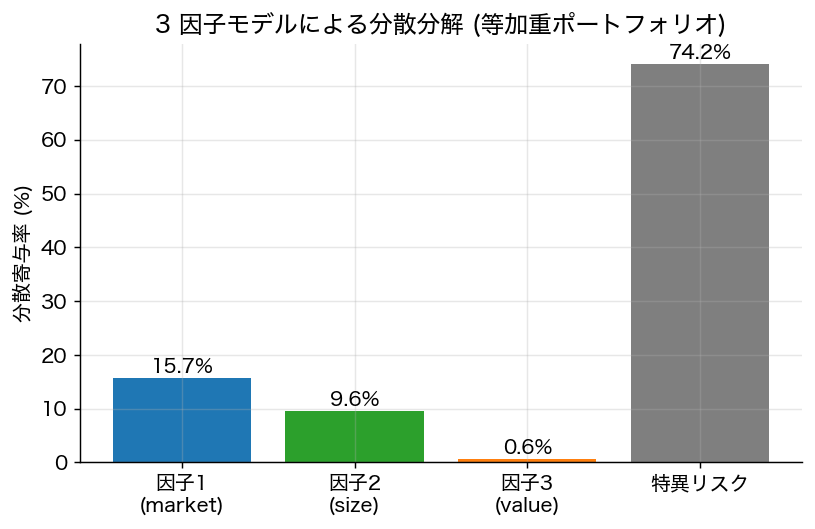
\includegraphics[width=0.85\linewidth]{figures/factor_decomposition.png}
\caption{3 因子モデル下での等加重ポートフォリオの分散寄与率分解。市場因子が支配的で、特異リスクは $n=25$ 銘柄に分散され小さい。リスクの源泉を要因別に可視化することで、運用上の意思決定（特定因子へのヘッジなど）が可能になる。}
\end{figure}

\section{5.6 主成分分析（PCA）的因子}

「観察可能なファクター」ではなく、共分散行列の \textbf{主成分} を用いる手法（\textbf{統計的因子モデル}）。Chamberlain–Rothschild (1983) の \textbf{近似因子モデル} はその理論的基礎を与え、$\Sigma$ の固有値の発散順序によって「強い因子」と「弱い因子」を区別する。

\section{5.7 まとめ}

\begin{itemize}
\item APT は \textbf{無裁定 + 大数の法則} から多因子線形価格モデルを導く。
\item CAPM の 1 因子化は厳しい仮定。実証的には 3–5 因子が支持される。
\item 因子モデルは共分散行列推定・リスク管理・パフォーマンス分析の中核技術。
\end{itemize}

\noindent\hrulefill

% ===== 06_utility_theory.md =====
\chapter{第6章 効用理論と期待効用}

平均分散分析は「リターンの平均と分散だけが効用に影響する」という強い前提に立つ。一般的にこれが正当化されるのは

\begin{itemize}
\item 投資家の効用関数が \textbf{二次} であるか、
\item リターン分布が \textbf{楕円的} であるか、
\end{itemize}

のどちらかのときだけである。本章ではより一般の期待効用理論を概観する。

\section{6.1 von Neumann–Morgenstern の公理}

確率くじ（lottery）$L \in \mathcal{L}$ 上の選好関係 $\succeq$ に対し、次の四公理：

\begin{enumerate}
\item \textbf{完備性（completeness）}
\item \textbf{推移性（transitivity）}
\item \textbf{連続性（continuity）}
\item \textbf{独立性（independence）}：$L_1 \succeq L_2 \Rightarrow \alpha L_1 + (1-\alpha) L_3 \succeq \alpha L_2 + (1-\alpha) L_3$。
\end{enumerate}

\textbf{定理 6.1}（vNM 期待効用表現定理） 上記四公理を満たす選好関係に対し、効用関数 $u: \mathbb{R} \to \mathbb{R}$（アフィン変換を除いて一意）が存在し \[ L_1 \succeq L_2 \iff \mathbb{E}_{L_1}[u(X)] \ge \mathbb{E}_{L_2}[u(X)]. \]

\emph{証明方針}：標準的くじ $\{p \cdot \bar W + (1-p) \cdot \underline W\}$ を参照基準とし、独立性公理を用いて任意のくじを「ある $p$ の標準くじと等価」と見なせる（無差別変換）。この $p$ が効用 $u(X)$ の正当な候補となる。連続性で滑らかさを担保。$\square$

\section{6.2 リスク回避}

\textbf{定義 6.2}
\begin{itemize}
\item 投資家が \textbf{リスク回避的} $\iff$ 任意の非退化くじ $X$ に対し $u(\mathbb{E}[X]) \ge \mathbb{E}[u(X)]$。
\item これは Jensen の不等式より $u$ が \textbf{凹} であることと同値。
\end{itemize}

!\href{figures/jensen\_inequality.png}{Jensen の不等式の視覚化：凹な効用 $u$ の下で、くじ $\{W_1, W_2\}$ の期待効用 $\mathbb{E}[u(W)]$（弦の中点）は確実な期待値 $\mathbb{E}[W]$ の効用 $u(\mathbb{E}[W])$（曲線上の点）より下にある。リスク回避と凹性の同値性が幾何的に見える。}

\textbf{定義 6.3}（Arrow–Pratt のリスク回避度）
\begin{itemize}
\item \textbf{絶対リスク回避度（ARA）}：$A(W) := -u''(W) / u'(W)$。
\item \textbf{相対リスク回避度（RRA）}：$R(W) := -W u''(W) / u'(W)$。
\end{itemize}

\textbf{直観}：危険資産への投資量 $\alpha^\star$ を二次近似で展開すると（小リスク近似） \[ \alpha^\star \approx \frac{\mathbb{E}[R - r_f]}{A(W)\, \sigma_R^2}. \]

\section{6.3 標準効用関数}

\begin{center}
\begin{tabular}{|l|l|l|l|}
\hline
効用 & 関数形 & ARA & RRA \\ \hline
指数（CARA） & $-e^{-\gamma W}/\gamma$ & $\gamma$（一定） & $\gamma W$ \\ \hline
べき（CRRA） & $W^{1-\gamma}/(1-\gamma)$, $\gamma\neq 1$ & $\gamma/W$ & $\gamma$（一定） \\ \hline
対数 & $\log W$ & $1/W$ & $1$ \\ \hline
二次 & $W - \tfrac{\gamma}{2}W^2$ & $\gamma/(1-\gamma W)$ & 増加 \\ \hline
\end{tabular}
\end{center}

\textbf{CARA（指数）効用} は富水準に依存せず投資量が一定。\textbf{CRRA（べき・対数）} は富比例で投資する（\textbf{実証的に支持}）。二次効用は飽和（$W > 1/\gamma$ で逆転）するため理論的に都合悪い。

\begin{figure}[H]
\centering
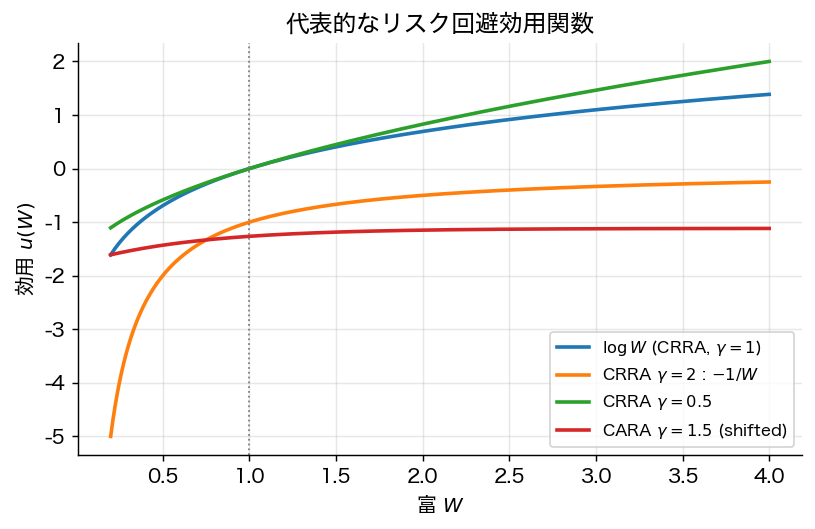
\includegraphics[width=0.85\linewidth]{figures/utility_functions.png}
\caption{代表的なリスク回避効用関数の比較。CRRA $\gamma=2$ は曲率が大きく、$\gamma$ が小さいほど線形に近づく（リスク中立に近い）。すべて凹関数だが、曲率の差がリスク回避度の差を生む。}
\end{figure}

\section{6.4 平均分散効用と期待効用の整合性}

\textbf{命題 6.4} リターンが \textbf{多変量正規分布} に従い、効用が CARA 型 $u(W) = -e^{-\gamma W}$ であるとき、期待効用最大化は \textbf{平均分散最適化} と完全に等価： \[ \max_w \mathbb{E}[u(W_0 + w^\top R)] \iff \max_w \left\{ w^\top \mu - \tfrac{\gamma W_0}{2}\, w^\top \Sigma w\right\}. \]

\emph{証明方針}：$X \sim \mathcal{N}(m, s^2)$ のとき積率母関数 $\mathbb{E}[e^{-\gamma X}] = \exp(-\gamma m + \gamma^2 s^2/2)$ を用いる。$\square$

これが Markowitz 理論の理論的正当化の核心。\textbf{正規分布の仮定が崩れる}（重尾、歪み、ジャンプ）と平均分散は近似でしかなくなる。

\section{6.5 高次モーメントの取り込み}

3 次（歪度）・4 次（尖度）モーメントを考慮した効用展開： \[ \mathbb{E}[u(W)] \approx u(\bar W) + \tfrac{1}{2} u''\sigma^2 + \tfrac{1}{6} u'''\, \mu_3 + \tfrac{1}{24} u''''\, \mu_4 + \cdots \]

$u''' > 0$（"prudence"）は \textbf{正の歪度を好む}、$u'''' < 0$（"temperance"）は \textbf{大きな尖度を嫌う}。実証的に投資家はそうした選好を示し、宝くじ的（プラス歪度）資産が「高すぎる」価格を持つ現象を生む。

\section{6.6 行動経済学的代替}

vNM 期待効用は \textbf{Allais のパラドックス} 等で実験的に反証される。代替モデル：

\begin{itemize}
\item \textbf{プロスペクト理論}（Kahneman–Tversky 1979）：参照点依存、損失回避（loss aversion）、確率歪曲関数。
\item \textbf{累積プロスペクト理論}（1992）：確率歪曲を累積分布関数に作用させる。
\item \textbf{ランク依存効用}（Quiggin 1982）。
\end{itemize}

これらは「ボラティリティ・スマイル」「モメンタム」など金融市場アノマリの説明候補となる。

\section{6.7 まとめ}

\begin{itemize}
\item 期待効用最大化は vNM 四公理から導かれる。
\item リスク回避は効用の凹性、ARA/RRA で定量化。
\item 平均分散 = 期待効用 となるのは正規分布 + CARA / 二次効用のとき。
\item 実際にはより一般の効用（CRRA、行動）と分布（非正規）が必要。
\end{itemize}

\noindent\hrulefill

% ===== 07_stochastic_dominance.md =====
\chapter{第7章 確率支配}

平均分散だけでは捉えきれない「選好」のうち、ほぼ全ての合理的投資家が同意する \textbf{頑健な順序付け} が確率支配である。

\section{7.1 一次確率支配（First-order Stochastic Dominance; FSD）}

\textbf{定義 7.1} 確率変数 $X, Y$ について $X \succeq_{\rm FSD} Y$ とは、$F_X(t) \le F_Y(t)$ がすべての $t$ で成立すること。すなわち $X$ の累積分布関数が $Y$ より「下にある」。

\textbf{定理 7.2} $X \succeq_{\rm FSD} Y \iff \mathbb{E}[u(X)] \ge \mathbb{E}[u(Y)]$ がすべての \textbf{単調非減少関数} $u$ に対して成立。

\emph{証明方針}：
\begin{itemize}
\item ($\Leftarrow$) $u(t) = \mathbf{1}_{t > s}$ という指示関数（極限的に単調）を取ると $\mathbb{E}[u(X)] = 1 - F_X(s)$、これが全 $s$ で $\ge 1 - F_Y(s)$。
\item ($\Rightarrow$) $u$ が単調非減少なら $u(t) = \int \mathbf{1}_{t > s} \mu(ds)$（Stieltjes 積分表示）で書け、各 indicator で成立する不等式を線形結合。$\square$
\end{itemize}

すなわち FSD は「より多くを好む」全ての投資家が同意する順序。

\section{7.2 二次確率支配（Second-order Stochastic Dominance; SSD）}

\textbf{定義 7.3} $X \succeq_{\rm SSD} Y$ とは $\int_{-\infty}^t F_X(s) ds \le \int_{-\infty}^t F_Y(s) ds$ が全 $t$ で成立すること。

\textbf{定理 7.4} $X \succeq_{\rm SSD} Y \iff \mathbb{E}[u(X)] \ge \mathbb{E}[u(Y)]$ がすべての \textbf{単調非減少凹関数} $u$ に対して成立。

\emph{証明方針}：
\begin{itemize}
\item ($\Leftarrow$) $u(t) = -(s - t)^+$（凹かつ単調非減少）に対する期待値が CDF の積分で書けることを示す（部分積分）。
\item ($\Rightarrow$) 任意の単調凹 $u$ を $-(s-t)^+$ 型関数の凸結合として近似（Riemann 和分解、Hardy–Littlewood–Pólya の補題）。$\square$
\end{itemize}

すなわち SSD は \textbf{「より多くを好み、かつリスク回避的な」全投資家} が同意する順序。

\textbf{重要な系}：$\mathbb{E}[X] = \mathbb{E}[Y]$ かつ $\mathrm{Var}(X) \le \mathrm{Var}(Y)$ でも、$X \succeq_{\rm SSD} Y$ は \textbf{一般には成立しない}（高次モーメントの効果）。逆に正規分布族の中では平均分散順序＝SSD 順序。

\begin{figure}[H]
\centering
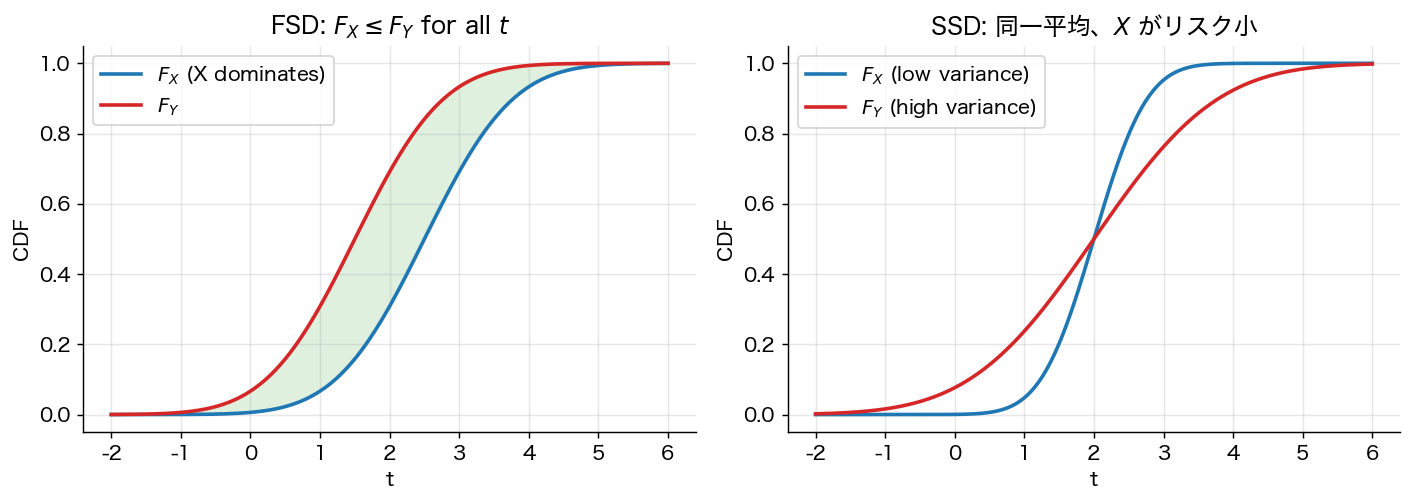
\includegraphics[width=0.85\linewidth]{figures/stochastic_dominance.png}
\caption{FSD と SSD の累積分布関数による特徴付け。左：FSD では $F_X(t) \le F_Y(t)$ が全 $t$ で成立（$X$ の CDF が常に下）。右：SSD は同じ平均で分散が小さい方が CDF 積分の意味で支配する。}
\end{figure}

\section{7.3 リスクのない/あるリスクの増大（Rothschild–Stiglitz 1970）}

\textbf{定義 7.5} $Y$ が $X$ の \textbf{平均保存スプレッド（mean-preserving spread; MPS）} であるとは、$\mathbb{E}[X] = \mathbb{E}[Y]$ かつ $Y \stackrel{d}{=} X + \varepsilon$（$\varepsilon$ は条件付き平均ゼロのノイズ）と表せること。

\textbf{定理 7.6}（Rothschild–Stiglitz） 以下は同値：
\begin{enumerate}
\item $Y$ は $X$ の MPS
\item $X \succeq_{\rm SSD} Y$（同一平均下で）
\item 全てのリスク回避効用 $u$ について $\mathbb{E}[u(X)] \ge \mathbb{E}[u(Y)]$
\end{enumerate}

\emph{証明方針}：MPS の構成性（独立ノイズ重ね合わせ）と Jensen の不等式の繰り返し適用、および「条件付き平均ゼロのノイズ追加」が Hardy–Littlewood–Pólya 型の majorization を生むこと。$\square$

\section{7.4 平均分散効率性と SSD の関係}

\textbf{事実 7.7}
\begin{itemize}
\item リターンが \textbf{多変量正規} な世界では：「平均分散効率」⇔「SSD 効率」⇔「ある CARA リスク回避者の最適化」。
\item 非正規世界では：平均分散効率は SSD 効率の \textbf{必要条件ではない}。実際、平均分散効率なポートフォリオが SSD で支配されることがある（例：ポジティブ歪度資産を排除するケース）。
\end{itemize}

これが「Markowitz 最適化が常に賢いとは限らない」具体的な根拠となる。

\section{7.5 高次の確率支配}

\textbf{$n$ 次確率支配} は順次積分した分布関数の比較で定義され、$u, u'', u^{(4)}, \dots$ の符号についての条件を満たす全ての効用に対応する。3 次以上は \textbf{慎重度（prudence）} や \textbf{節制（temperance）} といった高次性質と関連する。

\section{7.6 実用上の意義}

\begin{itemize}
\item \textbf{退職基金管理}：SSD 効率ポートフォリオを選ぶことで、加入者の効用関数を特定せずに「合理的な誰にとっても劣らない」運用を保証できる。
\item \textbf{オプション戦略}：プレミアム支払い・限定上限の戦略は平均分散では劣ることがあっても SSD では支配する/されない複雑な構造を持つ。
\end{itemize}

\section{7.7 まとめ}

\begin{itemize}
\item FSD：単調効用全体に対する順序（ほぼ普遍的）。
\item SSD：単調凹効用全体に対する順序（リスク回避者全員）。
\item MPS と SSD は同値（Rothschild–Stiglitz）。
\item 平均分散効率 ≠ SSD 効率（非正規分布下）。
\end{itemize}

\noindent\hrulefill

% ===== 08_risk_measures.md =====
\chapter{第8章 リスク尺度}

\begin{quote}
🎯 \textbf{この章で答える問い}
- 「リスク」を \textbf{標準偏差以外} で測る理由は何か。
- 銀行・保険会社が使う \textbf{VaR} はなぜ批判されたのか。
- \textbf{CVaR (Expected Shortfall)} はなぜ規制で標準になったのか。

📐 \textbf{使う数学}：分位点・確率分布の裾、期待値の線形性。

🔑 \textbf{主要結果}：VaR は劣加法性を欠くため分散投資をペナルティしうるが、CVaR は劣加法性を満たし「\textbf{合理的なリスク尺度}」（Artzner 公理）として規制で標準になった。
\end{quote}

\section{8.1 リスク尺度とは何か}

リスク尺度 $\rho$ は損失分布 $L$ に実数 $\rho(L)$ を対応させる写像。標準偏差はその一例だが、

\begin{itemize}
\item 損失の \textbf{左裾（テールリスク）} に十分敏感でない
\item 対称な指標であり「損益の非対称性」を捉えない
\item 規制目的では \textbf{必要資本量} の解釈が直接できない
\end{itemize}

これらの欠点を補うのが本章のテーマである。

\section{8.2 Value-at-Risk (VaR)}

\textbf{定義 8.1} 損失 $L$ の信頼水準 $\alpha \in (0, 1)$ における VaR は \[ \mathrm{VaR}_\alpha(L) := \inf\{ x \in \mathbb{R} : P(L > x) \le 1 - \alpha\} = F_L^{-1}(\alpha) \] 通常 $\alpha = 0.95$ や $0.99$。

\textbf{バーゼル規制等で長年標準だった}。しかし以下の欠点を持つ。

\begin{figure}[H]
\centering
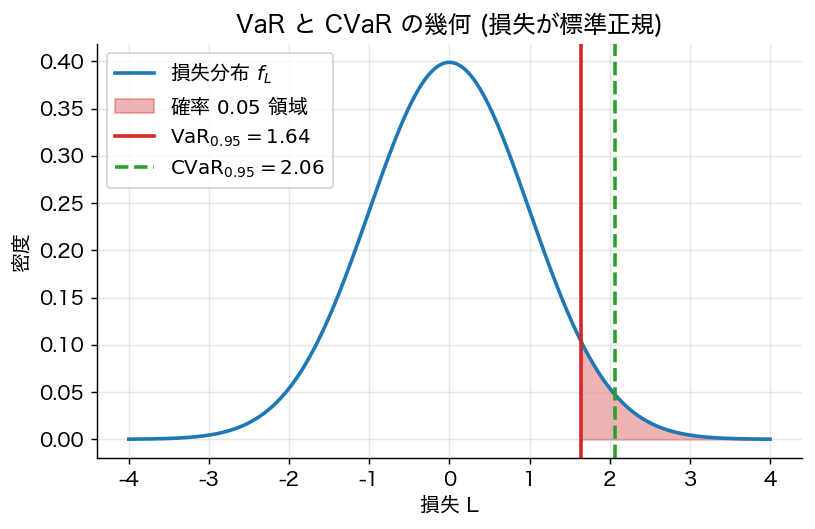
\includegraphics[width=0.85\linewidth]{figures/var_cvar.png}
\caption{VaR と CVaR の幾何的意味（損失が標準正規の場合）。VaR は分位点で「テールの境界」だけを見るのに対し、CVaR は分位点を超えた領域の \textbf{平均} を取るため、テール形状の情報を保持する。}
\end{figure}

\section{8.3 VaR の問題点：非劣加法性}

\textbf{事実 8.2} VaR は一般に \textbf{劣加法性}（$\rho(L_1 + L_2) \le \rho(L_1) + \rho(L_2)$）を満たさない。すなわち分散投資により VaR が悪化することがある。

\textbf{反例（独立性を仮定）}：\textbf{独立} な 2 つのデフォルト債を考える。各々 $P(\text{損失}=100) = 0.04$、$P(0) = 0.96$。$\alpha = 0.95$ で個別 VaR はいずれも 0。しかし合算 $L_1 + L_2$ の損失分布は $P(L=200) = 0.0016$, $P(L=100) = 2 \cdot 0.04 \cdot 0.96 = 0.0768$, $P(L=0) = 0.9216$。よって $\mathrm{VaR}_{0.95}(L_1 + L_2) = 100 > 0 + 0 = \mathrm{VaR}(L_1) + \mathrm{VaR}(L_2)$。

これは「分散投資をペナルティする」異常な振る舞いで、合理的なリスク管理に反する。

\begin{quote}
⚠️ \textbf{実務注意 box：周辺分布だけでは VaR の合算は決まらない}

上の反例は \textbf{独立} を仮定した。$L_1, L_2$ の同時分布（相関や依存関係）が変わると、$L_1 + L_2$ の分布も変わり、合算 VaR の値も変わる。「個別資産の VaR だけからポートフォリオの VaR は計算できない」というのが、現代リスク管理の出発点である。一般に依存構造は \textbf{コピュラ} という道具で記述される（学部生は名前を覚えておけば十分）。
\end{quote}

\begin{figure}[H]
\centering
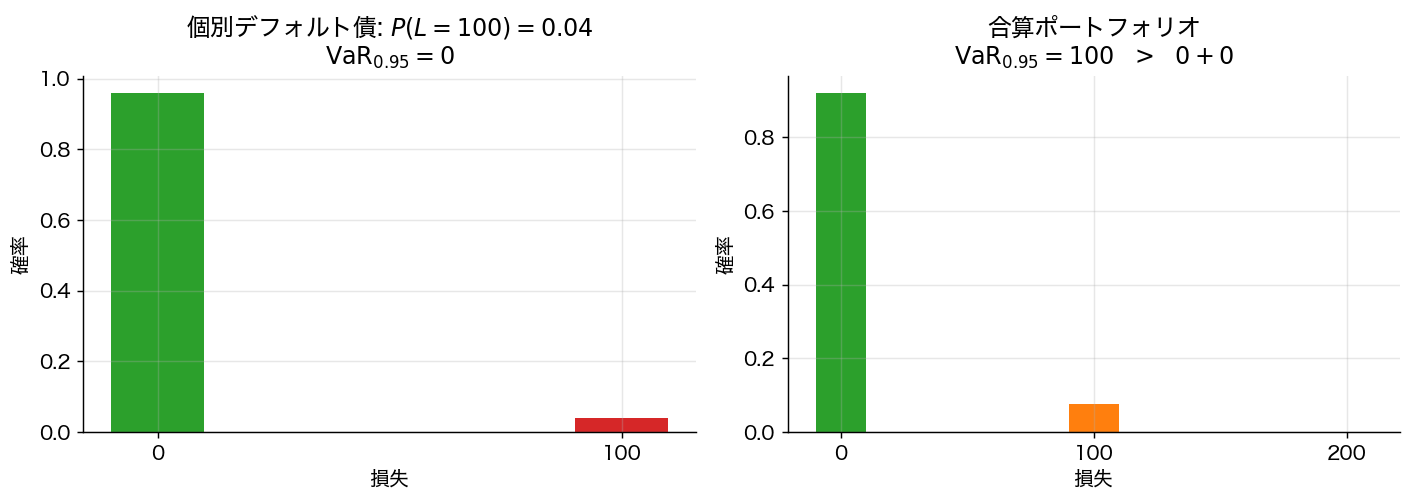
\includegraphics[width=0.85\linewidth]{figures/var_subadditivity.png}
\caption{VaR の劣加法性違反例（独立 2 デフォルト債）。左：個別の損失分布、$\mathrm{VaR}_{0.95}=0$。右：合算した分布で $\mathrm{VaR}_{0.95}=100$ となり、$0+0$ を超える。分散投資が VaR を悪化させる典型例。}
\end{figure}

\section{8.4 コヒーレントリスク尺度（Artzner et al. 1999）}

\textbf{定義 8.3}（コヒーレントリスク尺度） $\rho$ が次の四公理を満たすとき：
\begin{enumerate}
\item \textbf{単調性}：$L_1 \le L_2$ a.s. $\Rightarrow \rho(L_1) \le \rho(L_2)$
\item \textbf{平行移動不変性}：$\rho(L + c) = \rho(L) + c$（$c$ は確定損失）
\item \textbf{正同次性}：$\rho(\lambda L) = \lambda \rho(L)$（$\lambda \ge 0$）
\item \textbf{劣加法性}：$\rho(L_1 + L_2) \le \rho(L_1) + \rho(L_2)$
\end{enumerate}

\textbf{動機}：四公理は数学的趣味ではなく、「\textbf{合算・分散・資本配賦に耐えるリスク尺度の条件}」として読むべきである。例えば：
\begin{itemize}
\item 単調性：損失が確実に大きい資産は確実にリスクが大きい。
\item 平行移動不変性：「確定損失 $c$ を足したらリスクは $c$ 増える」（資本要件として直観的）。
\item 劣加法性：「分散投資すればリスクは減るか同じ」（最重要、VaR が破る性質）。
\item 正同次性：ポジション 2 倍ならリスク 2 倍（流動性無視の単純化）。
\end{itemize}

\begin{quote}
🛣 \textbf{上級学習への道標：コヒーレント尺度の双対表現}

コヒーレント性公理を満たす $\rho$ は、ある「シナリオ確率測度の集合 $\mathcal{Q}$」を用いて
\[ \rho(L) = \sup_{Q \in \mathcal{Q}} \mathbb{E}_Q[L] \]
と書ける（\textbf{Artzner et al. 1999} の双対表現定理）。「最悪シナリオでの期待損失」という直観的解釈を持つ。証明は \textbf{凸解析の Hahn–Banach 分離定理} を要するため本書では割愛。詳しくは Föllmer \& Schied \emph{Stochastic Finance} (2016) を参照。
\end{quote}

\section{8.5 Conditional VaR / Expected Shortfall}

\textbf{定義 8.5} \[ \mathrm{CVaR}_\alpha(L) = \mathbb{E}[L \mid L \ge \mathrm{VaR}_\alpha(L)] \] （厳密には離散的分布の場合の取扱いに注意、Rockafellar–Uryasev 2000 を参照）。同義：Expected Shortfall (ES)、Tail VaR、Average VaR。

\textbf{定理 8.6} CVaR は \textbf{コヒーレント} リスク尺度（特に劣加法性を満たす）。

\textbf{直観}：CVaR は「テールを超えた損失の \textbf{平均}」なので、線形性（期待値の性質）から劣加法性 $\mathrm{CVaR}(L_1 + L_2) \le \mathrm{CVaR}(L_1) + \mathrm{CVaR}(L_2)$ が自然に従う。VaR が分位点（順序統計量）であるのに対し、CVaR は \textbf{平均} なので「足し算と相性が良い」。厳密な証明はテール条件付き期待値の凸性を使う。

\textbf{実務的利点}：
\begin{itemize}
\item 劣加法性のため分散投資を促進する。
\item 凸最適化と相性が良い（Rockafellar–Uryasev による線形計画化）。
\item 損失の \textbf{平均的な大きさ} を測るため、テールリスクの情報を保つ。
\end{itemize}

バーゼル III から CVaR が市場リスク資本計算の標準指標となった。

\section{8.6 CVaR 最適化（Rockafellar–Uryasev）}

\textbf{定理 8.7} ポートフォリオ $w$ の損失 $L_w(R) = -w^\top R$ の CVaR は補助関数 \[ F_\alpha(w, \zeta) := \zeta + \frac{1}{1-\alpha}\, \mathbb{E}[(L_w - \zeta)^+] \] について $\mathrm{CVaR}_\alpha(L_w) = \min_\zeta F_\alpha(w, \zeta)$。さらに $(w, \zeta)$ について同時最小化が可能で \textbf{凸最適化}（リターン分布が標本表現なら \textbf{線形計画問題}）に帰着する。

\emph{証明方針}：$\zeta = \mathrm{VaR}_\alpha$ で最小達成、これは凸関数の劣勾配法で示せる。標本表現 $R \in \{R^{(1)}, \dots, R^{(S)}\}$ では $(L_w^{(s)} - \zeta)^+ = u_s$、$u_s \ge 0$、$u_s \ge L_w^{(s)} - \zeta$ の線形緩和で書ける。$\square$

これにより、\textbf{シナリオベース CVaR 最小化} は LP ソルバで効率的に解ける。

\section{8.7 まとめ}

\begin{itemize}
\item VaR は実務標準だったが \textbf{劣加法性を欠き、分散投資をペナルティしうる}。
\item CVaR は「テール平均」として劣加法性を満たし、凸最適化と相性が良い。
\item Artzner 公理は「合理的なリスク尺度の最低条件」を与える設計指針。
\item ポートフォリオの合算リスクは個別 VaR だけでは決まらず、\textbf{依存構造（コピュラ）} が必要。
\end{itemize}

\begin{quote}
🛣 \textbf{上級学習への道標}
- \textbf{スペクトラルリスク尺度・歪曲リスク尺度}：CVaR を一般化し、テールに重みを連続的に置ける（Acerbi 2002）。
- \textbf{凸リスク尺度（Föllmer–Schied 2002）}：劣加法性 + 正同次性を弱めた凸性に置き換えると、流動性リスク・大ポジションの非線形効果を扱える。
- \textbf{動的・時間整合リスク尺度}（Cheridito–Delbaen–Kupper 2006, Ruszczyński 2010）：複数期間にわたるリスクを \textbf{入れ子型条件付期待値} で書く。
- \textbf{コピュラ理論}：周辺分布と依存構造を分離して合算リスクを扱う（McNeil–Frey–Embrechts \emph{Quantitative Risk Management} 2015）。
\end{quote}

\noindent\hrulefill

% ===== 09_black_litterman.md =====
\chapter{第9章 Black–Litterman モデル}

Markowitz 最適化は推定誤差を増幅する（\textbf{極端なロングショート}、\textbf{入力に対する高感度}）。Black \& Litterman (1992) は \textbf{均衡を事前情報、投資家の主観的見方を観測情報} とするベイズ枠組みで、この問題を本質的に解決した。

\section{9.1 出発点：暗黙の均衡リターン}

平均分散最適化を逆向きに使う：\textbf{現実の市場ポートフォリオ $w^M$}（時価総額比例）を「均衡における最適解」と見なし、それを生成する \textbf{暗黙の期待リターン} $\Pi$ を逆算する。

平均分散効用 $U(w) = w^\top\mu - \tfrac{\gamma}{2} w^\top \Sigma w$ の最適性条件 $w^\star = \gamma^{-1} \Sigma^{-1} (\mu - r_f\mathbf{1})$ より \[ \boxed{\; \Pi = \gamma\, \Sigma\, w^M + r_f \mathbf{1} \;} \] （\textbf{Sharpe’s implied returns} とも呼ぶ）。$\gamma$ は市場全体のリスク回避度。

\section{9.2 ベイズ的見方の取り込み}

投資家は \textbf{$K$ 本の主観的な見方（views）} を持つとする。これを線形等式 \[ P \mu = Q + \eta, \qquad \eta \sim \mathcal{N}(0, \Omega) \] で表現する。
\begin{itemize}
\item $P \in \mathbb{R}^{K\times n}$：各見方が「どの資産の組合せ」に関わるか。
\item $Q \in \mathbb{R}^K$：見方の \textbf{期待値}。
\item $\Omega \in \mathbb{R}^{K\times K}$：見方の \textbf{不確実性}（対角成分が大きいほど自信が薄い）。
\end{itemize}

\textbf{例}：
\begin{itemize}
\item 「資産 A は資産 B より 3\% 高い」→ $P$ の行は $(0, \dots, 1, \dots, -1, \dots, 0)$、$Q = 0.03$。
\item 「資産 C は絶対的に 8\% のリターンを上げる」→ $P$ の行は単位ベクトル、$Q = 0.08$。
\end{itemize}

\section{9.3 事前分布と事後分布}

\textbf{事前}：$\mu \sim \mathcal{N}(\Pi, \tau \Sigma)$。スケール $\tau$ は均衡への自信度を制御（典型的に $\tau \in [0.025, 0.05]$）。

\textbf{観測}：$P \mu \sim \mathcal{N}(Q, \Omega)$。

これらをベイズ更新する。

\textbf{定理 9.1}（Black–Litterman の事後分布） 事後分布 $\mu | \text{views}$ は正規分布で、 \[ \boxed{\; \hat\mu_{\rm BL} = \bigl[(\tau\Sigma)^{-1} + P^\top \Omega^{-1} P \bigr]^{-1}\bigl[(\tau\Sigma)^{-1} \Pi + P^\top \Omega^{-1} Q\bigr] \;} \] \[ \hat\Sigma_{\rm BL,\mu} = \bigl[(\tau\Sigma)^{-1} + P^\top \Omega^{-1} P\bigr]^{-1}. \]

\emph{証明方針}：正規 × 正規の共役事前分布更新。完全平方の項を整理すれば二次形式の精度行列が和、平均が精度加重和になる標準結果。$\square$

\textbf{等価な書き直し}（数値的により安定）： \[ \hat\mu_{\rm BL} = \Pi + \tau\Sigma P^\top (P \tau\Sigma P^\top + \Omega)^{-1} (Q - P\Pi). \]

\section{9.4 リターン分布とポートフォリオ最適化}

リターン自体の事後分布は \[ R | \text{views} \sim \mathcal{N}\bigl(\hat\mu_{\rm BL},\ \Sigma + \hat\Sigma_{\rm BL,\mu}\bigr) \] （推定不確実性を加える）。

平均分散最適化に代入して、\textbf{事後ポートフォリオ} \[ w^\star_{\rm BL} = \frac{1}{\gamma}(\Sigma + \hat\Sigma_{\rm BL,\mu})^{-1}(\hat\mu_{\rm BL} - r_f\mathbf{1}). \]

実務的には $\Sigma$ のみを使う簡略版もよく見られる。

\begin{figure}[H]
\centering
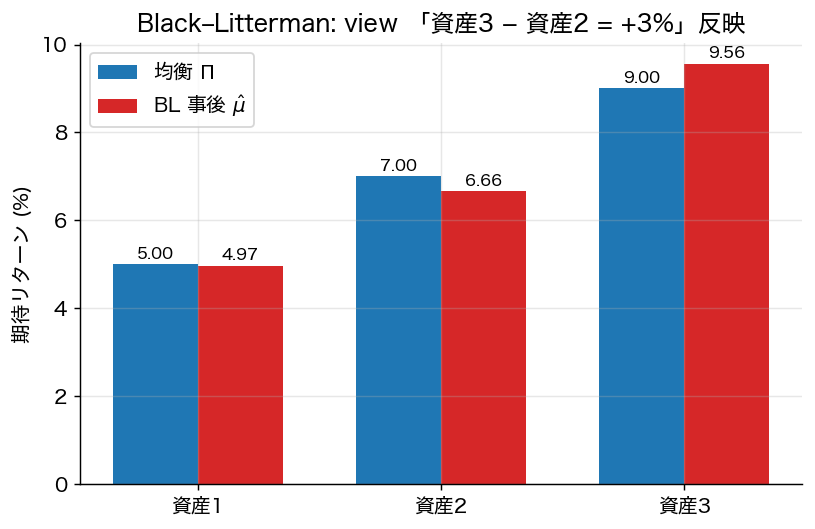
\includegraphics[width=0.85\linewidth]{figures/black_litterman.png}
\caption{Black–Litterman による期待リターンのベイズ的更新例。view「資産 3 − 資産 2 = +3\%」を反映して、資産 3 の事後リターンが上方修正され、資産 2 は下方修正される。view に関与しない資産 1 も共分散経由でわずかに更新される点に注目。}
\end{figure}

\section{9.5 Black–Litterman の魅力}

\begin{enumerate}
\item \textbf{見方を持たない資産は市場ウェイトに留まる}：$P$ にゼロを置けば、対応資産の事後は事前のまま。これにより極端な配分が抑制される。
\item \textbf{見方の自信度を $\Omega$ で連続的に調整}：$\Omega \to 0$ で見方を確信、$\Omega \to \infty$ で市場のまま。
\item \textbf{理論的に正当}：ベイズ統計の正規共役更新。
\item \textbf{実用上ロバスト}：均衡を事前にすることで「ノイズに乗っとられない」推定。
\end{enumerate}

\section{9.6 $\Omega$ の設定法}

BL 原論文は明示せず、後に複数提案：

\begin{itemize}
\item \textbf{Idzorek の方法}：各見方の「信頼度パーセンテージ」を入力すれば $\Omega$ を逆算。
\item \textbf{He–Litterman}：$\Omega = \mathrm{diag}(P \tau\Sigma P^\top)$（事前不確実性に比例）。
\item \textbf{Meucci の entropy pooling}：相対エントロピー最小化で見方を反映。
\end{itemize}

\section{9.7 例（数値例）}

3 資産（米国株、欧州株、日本株）、$\gamma = 2.5$ とする。
\begin{itemize}
\item 市場ウェイト $w^M = (0.6, 0.3, 0.1)$
\item 共分散 $\Sigma$ から $\Pi = \gamma\Sigma w^M + r_f\mathbf{1}$ を計算
\item 見方：「日本株は欧州株より 2\% 高い」→ $P = (0, -1, 1)$, $Q = 0.02$
\end{itemize}

ベイズ更新後、日本株の事後リターンが上方修正され、欧州株は下方修正。最適配分は日本株を超過配分する形になる。

\section{9.8 拡張}

\begin{itemize}
\item \textbf{Meucci のエントロピー・プーリング}：非ガウス分布、不等式型 view も扱える。
\item \textbf{Robust BL}：見方そのものに不確実性集合を許す。
\item \textbf{動的 BL}：時系列で view を更新する Kalman フィルタ的枠組み。
\end{itemize}

\section{9.9 まとめ}

\begin{itemize}
\item Black–Litterman は「均衡＝事前、view＝観測」というベイズ枠組み。
\item 推定誤差問題を本質的に緩和し、実務的に頑健なポートフォリオを生む。
\item 数式的には正規共役更新の特殊形に過ぎないが、解釈と運用性の点で革新的。
\end{itemize}

\noindent\hrulefill

% ===== 10_continuous_time_merton.md =====
\chapter{第10章 連続時間最適化：Merton 問題}

\begin{quote}
🎯 \textbf{この章で答える問い}
- 「\textbf{今この瞬間} 持っている富のうち、何 \% をリスク資産に置くべきか」を時間連続で問うとどうなるか。
- 答えはなぜ静的 Markowitz と同じ形（$\Sigma^{-1}(\mu - r\mathbf{1})$）になるのか。
- 「リスク回避度 $\gamma$ が大きいほど現金多め、消費は富比例」というお馴染みの結論はどこから来るか。

📐 \textbf{使う数学}：Taylor 展開、確率変数の平均と分散、ラグランジュ未定乗数法。

⚠️ \textbf{本章の方針}：本格的な \textbf{HJB 方程式} や \textbf{Itô 解析} は学部 4 年向けには重すぎるため、本書では \textbf{「1 期間離散モデルを連続時間極限する」近似的導入} だけを示す。完全な厳密版は章末の道標を参照。
\end{quote}

Markowitz は単期的な静的問題を扱う。実際には投資家は \textbf{時間を通じて連続的に再配分} し、しかも \textbf{消費} も行う。Merton (1969, 1971) はこの問題を確率制御として定式化し、CRRA 効用下では閉形解を得た。本書では「1 期間モデルの極限」として Merton 解の主要な形（最適投資比率）を導く。

\section{10.1 市場モデル}

\begin{itemize}
\item 無リスク資産：1 期間で $1 + r \Delta t$ に成長。
\item 危険資産：1 期間のリターン $\Delta S / S = \mu \Delta t + \sigma \sqrt{\Delta t}\, \varepsilon$、$\mathbb{E}[\varepsilon] = 0$, $\mathbb{E}[\varepsilon^2] = 1$。
\end{itemize}

$\Delta t \to 0$ の極限が \textbf{幾何ブラウン運動}： \[ \frac{dS_t}{S_t} = \mu\, dt + \sigma\, dW_t. \] $W_t$ は \textbf{標準ブラウン運動}（連続だが微分不能、平均 0・分散 $t$ の連続時間ガウス過程）。

\begin{quote}
📐 \textbf{数学補足 box：ブラウン運動と幾何ブラウン運動}

ブラウン運動 $W_t$ は次の 3 性質で特徴づけられる：
1. $W_0 = 0$
2. 増分 $W_{t+s} - W_t \sim \mathcal{N}(0, s)$（分散が時間幅に比例）
3. 異なる時間帯の増分は独立

幾何ブラウン運動 $dS = \mu S\, dt + \sigma S\, dW$ は「対数リターン $\log S_t$ がブラウン運動 + ドリフト」となる過程。株価モデルとして最も基本的。
\end{quote}

\section{10.2 1 期間ポートフォリオ問題 → 連続時間極限}

時刻 $t$ で富 $X_t$ のうち比率 $\pi$ を危険資産、$(1-\pi)$ を無リスク資産に置く。短時間 $\Delta t$ の富の変化は

\[ \frac{\Delta X}{X} = \pi \cdot (\mu \Delta t + \sigma \sqrt{\Delta t}\, \varepsilon) + (1 - \pi) \cdot r \Delta t = [r + \pi(\mu - r)] \Delta t + \pi \sigma \sqrt{\Delta t}\, \varepsilon. \]

CRRA 効用 $u(W) = W^{1-\gamma}/(1-\gamma)$ を Taylor 展開： \[ \mathbb{E}[u(X + \Delta X)] \approx u(X) + u'(X) X \cdot \mathbb{E}\!\left[\frac{\Delta X}{X}\right] + \tfrac{1}{2} u''(X) X^2 \cdot \mathbb{E}\!\left[\left(\frac{\Delta X}{X}\right)^2\right]. \]

ここで \[ \mathbb{E}\!\left[\frac{\Delta X}{X}\right] = [r + \pi(\mu - r)] \Delta t, \qquad \mathbb{E}\!\left[\left(\frac{\Delta X}{X}\right)^2\right] = \pi^2 \sigma^2 \Delta t + o(\Delta t). \]

$\Delta t$ の 1 次まで残し、$u'(X) = X^{-\gamma}$, $u''(X) = -\gamma X^{-\gamma - 1}$ を代入して \textbf{$\pi$ について最大化} すべき主要項は \[ \pi (\mu - r) - \frac{\gamma}{2} \pi^2 \sigma^2. \]

一階条件 $\mu - r - \gamma \pi \sigma^2 = 0$ より \[ \boxed{\;\pi^\star = \frac{\mu - r}{\gamma \sigma^2}\;} \]

これが \textbf{Merton 最適投資比率} の主要部分。$\Delta t \to 0$ の極限で連続時間問題の解と一致する。

\begin{quote}
⚠️ \textbf{実務注意 box：これは「投資比率の近似的導入」であって厳密な Merton 解の導出ではない}

上の議論は「投資比率」のみを扱っている。消費を同時に最適化する完全な Merton 問題では、消費 $c$ も同オーダーで効くため、価値関数の時間微分 $V_t$、消費効用 $u(c)$、富減少項 $-c \cdot V_X$ を全部同時に含む \textbf{HJB 方程式} を解かねばならない。本節の式は「投資政策の形」を予感させる入門であり、厳密性は章末の道標に従う。
\end{quote}

\section{10.3 結論の解釈}

最適投資比率 $\pi^\star = (\mu - r)/(\gamma \sigma^2)$ について：

\begin{itemize}
\item \textbf{超過リターン $\mu - r$ が大きいほど投資を増やす}（当然）。
\item \textbf{ボラティリティ $\sigma$ の 2 乗で割る} ため、ボラが 2 倍になると投資は 1/4。
\item \textbf{リスク回避度 $\gamma$ が大きいほど投資を減らす}。$\gamma = 1$（対数効用）で「Kelly 基準」に一致。
\item \textbf{時間不変}：$\pi^\star$ は時刻にも富水準にも依存しない（CRRA 効用の同次性）。
\end{itemize}

多資産化：$\mu \in \mathbb{R}^n$, $\Sigma$ で \[ \pi^\star = \frac{1}{\gamma}\, \Sigma^{-1}(\mu - r \mathbf{1}). \] \textbf{第2章の接線ポートフォリオの方向と完全に一致}。これが「Markowitz の静的解が動的にもそのまま使える」という驚くべき事実である。

\begin{figure}[H]
\centering
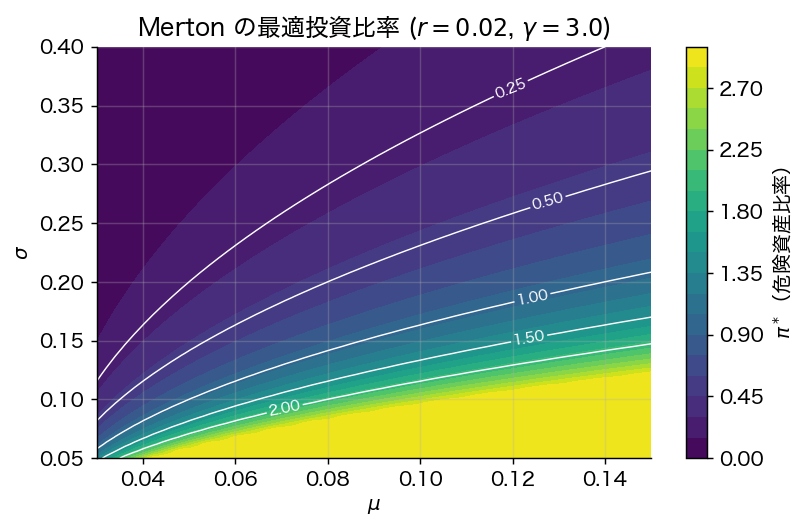
\includegraphics[width=0.85\linewidth]{figures/merton_policy.png}
\caption{Merton 問題の最適投資比率 $\pi^\star = (\mu-r)/(\gamma\sigma^2)$ を $(\mu, \sigma)$ 平面で等高線表示。ボラティリティが高いほど・期待リターンが低いほど危険資産投資を絞る。}
\end{figure}

\section{10.4 最適消費（結論のみ）}

完全な Merton 問題では「投資 + \textbf{消費}」を同時最適化する。本書では結果だけを述べる：

\textbf{事実 10.1}（Merton 1969, 結論のみ） CRRA 効用 $u(c) = c^{1-\gamma}/(1-\gamma)$, 主観割引率 $\rho$ の無限期間問題で、最適消費率は富に比例： \[ c^\star_t = m \cdot X_t, \qquad m = \frac{1}{\gamma}\left[\rho - (1 - \gamma)\left(r + \frac{(\mu - r)^2}{2 \gamma \sigma^2}\right)\right]. \]

直観：「\textbf{今期の消費} vs \textbf{投資して将来消費}」のトレードオフを取り、富比例で消費する政策が最適。富が増えれば消費も比例して増える（CRRA の同次性の帰結）。

\begin{figure}[H]
\centering
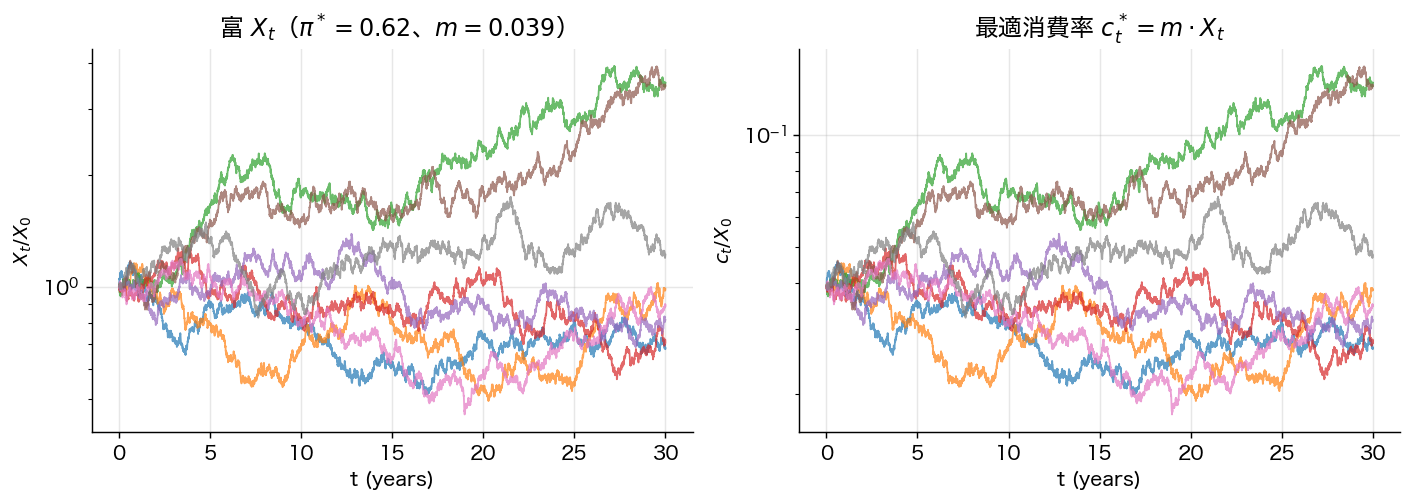
\includegraphics[width=0.85\linewidth]{figures/merton_paths.png}
\caption{Merton 問題の最適制御下での富経路と消費経路のシミュレーション（8 軌跡、$\mu=0.08, \sigma=0.18, r=0.02, \gamma=3$）。富は対数線形成長、消費は富に比例する。}
\end{figure}

\section{10.5 拡張トピック（概観のみ）}

実際の Merton 問題には多くの拡張がある。本書では結論だけ：

\begin{itemize}
\item \textbf{状態変数依存の市場（時変 $\mu, \sigma$）}：「\textbf{ヘッジ需要}」項が現れ、Merton (1973) の \textbf{異時点間 CAPM (ICAPM)} につながる。
\item \textbf{取引費用}：「\textbf{無取引帯}」を持つ最適政策（Davis–Norman 1990）。
\item \textbf{借入制約・空売り禁止}：自由境界問題に帰着。
\item \textbf{ジャンプ過程}：Merton (1976) のジャンプ拡散モデル。
\end{itemize}

\section{10.6 まとめ}

\begin{itemize}
\item 連続時間 Merton 問題の最適投資比率は \textbf{静的 Markowitz の接線方向と同じ}。
\item リスク回避度 $\gamma$ が高いほど現金多め、ボラティリティ 2 乗で投資を絞る。
\item 最適消費は富比例（CRRA 効用の帰結）。
\item 厳密な HJB 方程式・Itô 解析・確率制御は大学院修士課程の専門科目（[上級学習への道標] 参照）。
\end{itemize}

\begin{quote}
🛣 \textbf{上級学習への道標}
- \textbf{HJB 方程式と動的計画原理}：Karatzas \& Shreve \emph{Brownian Motion and Stochastic Calculus} (1991)、Pham \emph{Continuous-time Stochastic Control and Optimization with Financial Applications} (2009)。
- \textbf{マーチンゲール法（Cox–Huang 1989, Karatzas–Lehoczky–Shreve 1987）}：動的予算制約を \textbf{静的予算制約} に書き換える別解法。完全市場・凸双対の枠組み。
- \textbf{リスク中立測度との関係}：本章は実際の確率測度の下での投資問題。デリバティブ価格付けは「リスク中立」と呼ばれる別の確率測度を用いる（Black–Scholes–Merton 1973）。両者の関係は \textbf{確率割引因子 (SDF)} を介して理解できる（Cochrane \emph{Asset Pricing}, 2005）。
- 本書で省略した \textbf{消費を含む完全な導出} はラグランジュ + Bellman 方程式で行う。学部生にとっては Stokey \& Lucas \emph{Recursive Methods in Economic Dynamics} (1989) の離散版から入ると bridge しやすい。
\end{quote}

\noindent\hrulefill

% ===== 11_performance_evaluation.md =====
\chapter{第11章 運用パフォーマンスの評価}

ポートフォリオ運用の \textbf{事後評価} は、リスク調整リターンを定量化することで「運用者は実力か運か」「ベンチマークを超えたか」を問う活動である。本章は古典的指標と統計的検出力を解説する。

\section{11.1 Sharpe 比}

\textbf{定義 11.1}（Sharpe 1966） \[ \mathrm{SR} = \frac{\mathbb{E}[R_p] - r_f}{\sigma_p}. \]

CML の傾きそのものであり、第2章定理 2.3 の最大化対象。

\textbf{統計的推定}：標本サイズ $T$、独立 i.i.d 仮定下で \[ \hat{\mathrm{SR}} - \mathrm{SR} \sim \mathcal{N}\left(0,\ \frac{1 + \mathrm{SR}^2/2}{T}\right) \quad \text{(漸近)}. \] \emph{証明方針}：デルタ法 + 標本平均・標本分散の漸近正規性。$\square$

\textbf{注意}：リターンが \textbf{正規} という仮定が標準。歪度・尖度がある場合は Sharpe 比が不適切なことがある（Mertens 2002 補正、Lo 2002）。

\begin{figure}[H]
\centering
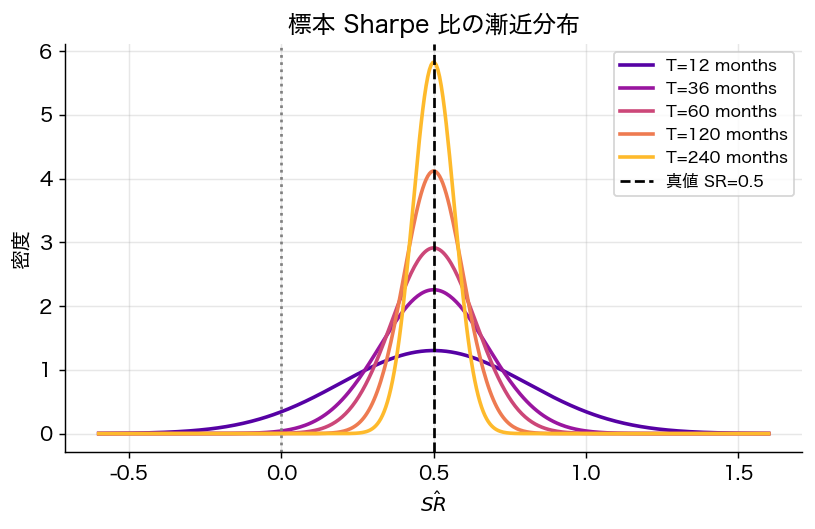
\includegraphics[width=0.85\linewidth]{figures/sharpe_distribution.png}
\caption{標本 Sharpe 比の漸近分布（真値 $\mathrm{SR}=0.5$、観測期間 $T$ ごと）。1〜3 年程度のデータでは「skill = 0」（真値ゼロ）と統計的に区別できない。長期データなしには運用者の skill を確信できないという、業界の本質的問題が見える。}
\end{figure}

\section{11.2 Treynor 比}

\[ \mathrm{Treynor} = \frac{\mathbb{E}[R_p] - r_f}{\beta_p}. \] 全分散の代わりに \textbf{β（市場リスク）} で割る。well-diversified なポートフォリオには適切だが、固有リスクが大きい場合に過大評価しがち。

\section{11.3 Jensen の α}

CAPM 回帰 \[ R_{pt} - r_{ft} = \alpha_p + \beta_p (R_{Mt} - r_{ft}) + \varepsilon_{pt} \] の切片 $\alpha_p$。CAPM が正しければ均衡で $\alpha = 0$ なので、$\alpha > 0$ は \textbf{「市場では説明できない超過リターン」}＝運用力（skill）の指標とされる。

\textbf{多因子 α}：Fama–French 3 因子回帰の切片で評価することで、サイズ・バリュー因子で説明される α を除外できる。

\section{11.4 情報比率（Information Ratio; IR）}

ベンチマーク $R_B$ に対する \textbf{アクティブリターン} $R_p - R_B$ について \[ \mathrm{IR} = \frac{\mathbb{E}[R_p - R_B]}{\mathrm{SD}(R_p - R_B)} = \frac{\alpha}{\sigma_\varepsilon}. \] \textbf{トラッキングエラー} で標準化された超過リターン。アクティブ運用の評価指標として最も重視される。

\section{11.5 Sortino 比}

下方リスクのみを罰する指標： \[ \mathrm{Sortino} = \frac{\mathbb{E}[R_p] - r_f}{\mathrm{SD}^-(R_p)}, \] ここで $\mathrm{SD}^-$ は下方半分散の平方根。投資家がアップサイドのボラを嫌わないなら理論的に Sharpe より整合的。

\section{11.6 最大ドローダウン・Calmar 比}

\textbf{最大ドローダウン}（MDD）：累積価値のピークから谷底までの最大下落率 \[ \mathrm{MDD} = \sup_{0 \le s \le t \le T} \left(1 - \frac{V_t}{V_s}\right). \] \textbf{Calmar 比} $= \mathbb{E}[R] / \mathrm{MDD}$（典型的に年率）。

\begin{figure}[H]
\centering
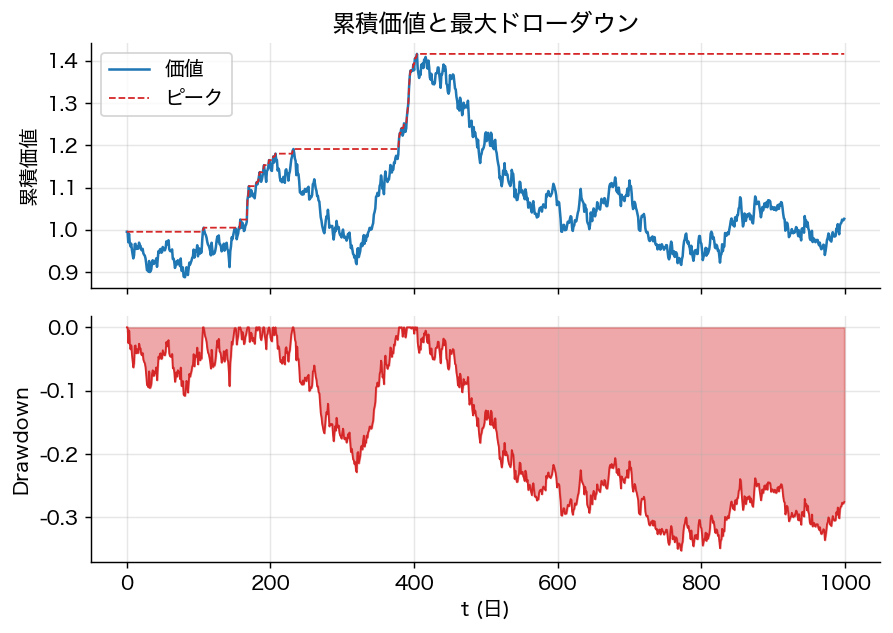
\includegraphics[width=0.85\linewidth]{figures/drawdown.png}
\caption{累積価値とドローダウンの可視化。上図：価値推移とピーク（赤破線）。下図：各時点のドローダウン。Sharpe 比だけでは現れない「投資家心理を試される深い谷」を Calmar 比で評価する。}
\end{figure}

\section{11.7 リスク調整パフォーマンスの数学的洞察}

\textbf{事実 11.2} 任意の運用戦略について、Sharpe 比は \textbf{時間にスケールする}： \[ \mathrm{SR}_{\text{年率}} = \sqrt{n} \cdot \mathrm{SR}_{\text{日次}} \] （独立同分布リターン仮定）。年率化は単純に $\sqrt{T}$ 倍。

\textbf{事実 11.3}（Bailey–López de Prado 2014） バックテストにおいて、複数の戦略から最良を選んだ「事後選択 Sharpe」は \textbf{大幅にバイアスがかかる}： \[ \mathbb{E}[\max_i \widehat{\mathrm{SR}}_i] \approx \sigma_{\mathrm{SR}} \cdot \sqrt{2\log N} \] （$N$ は戦略数）。\textbf{Deflated Sharpe Ratio} で補正が必要。

\section{11.8 検出力：必要サンプル}

「ある真の Sharpe 比が $\mathrm{SR}$ で正であるか有意性 5\%・検出力 80\% で確認するための最低期間」は概算 \[ T \gtrsim \frac{(1.96 + 0.84)^2 (1 + \mathrm{SR}^2/2)}{\mathrm{SR}^2}. \] たとえば $\mathrm{SR} = 0.5$ 年なら約 32 年必要。\textbf{多くのファンドが「実力か運か」統計的に判別不能}。

\section{11.9 リスク帰属・パフォーマンス帰属}

\begin{itemize}
\item \textbf{Brinson 分解}：超過リターンを「アロケーション効果・銘柄選択効果・相互作用効果」に分解。
\item \textbf{リスク要因帰属}：ファクターモデルで分散を要因別に分解。
\item \textbf{時系列回帰 α + 横断面回帰}：Fama–MacBeth 型評価。
\end{itemize}

\section{11.10 リスク調整指標の関係}

\begin{center}
\begin{tabular}{|l|l|l|l|}
\hline
指標 & リスク尺度 & ベンチマーク & 仮定 \\ \hline
Sharpe & 全分散 & 無リスク & 正規分布 \\ \hline
Treynor & β & 無リスク & 完全分散 \\ \hline
Jensen α & 残差分散 & CAPM & CAPM 妥当性 \\ \hline
IR & TE（残差分散） & 指数 & — \\ \hline
Sortino & 下方分散 & 目標 & 下方リスク選好 \\ \hline
\end{tabular}
\end{center}

\section{11.11 まとめ}

\begin{itemize}
\item Sharpe 比は最も普及した指標だが、正規分布・i.i.d 仮定に依存。
\item Jensen α と IR は α 検出に有用。
\item バックテスト Sharpe は \textbf{データスヌーピング} で著しくバイアス。
\item 統計的に skill を実証するには \textbf{長期データ＋多重比較補正} が必須。
\end{itemize}

\noindent\hrulefill

% ===== 12_shrinkage_rmt.md =====
\chapter{第12章 共分散行列の縮小推定と高次元漸近}

\begin{quote}
🎯 \textbf{この章で答える問い}
- 標本共分散 $S$ をそのまま使うと \textbf{なぜ Markowitz 最適化が暴れるのか}。
- 「\textbf{縮小推定（shrinkage）}」とはどんな技で、なぜ効くのか。
- $\Sigma = I$（真は単位行列）なのに \textbf{標本固有値が広く分布する} 現象（Marčenko–Pastur）の意味。

📐 \textbf{使う数学}：行列の固有値、対角化、Frobenius ノルム。

🔑 \textbf{主要結果}：Ledoit–Wolf 線形縮小 $\hat\Sigma = (1-\alpha) S + \alpha (\mathrm{tr}(S)/p) I$ は出力ポートフォリオを安定化させ、out-of-sample で勝つ。
\end{quote}

\section{12.1 大次元下の標本共分散行列の病理}

Markowitz の最適化は $\Sigma^{-1}$ を要求する。実務では母共分散 $\Sigma$ を観測できないので、$T$ 期間の標本 $R_1, \dots, R_T$ から \textbf{標本共分散行列} \[ S = \frac{1}{T-1} \sum_{t=1}^T (R_t - \bar R)(R_t - \bar R)^\top \] を用いる。古典的統計では $p$（資産数）固定で $T \to \infty$ なら $S \to \Sigma$（Wishart の一致性）。しかし実務では $p$ と $T$ が同程度のオーダー、典型的には $p/T \approx 0.5$–$2.0$。この \textbf{大次元} 領域では破綻が起こる。

\textbf{事実 12.1}（Marčenko–Pastur 1967） $\Sigma = I_p$（真の共分散が単位行列）、$p/T \to c \in (0, \infty)$ のとき、$S$ の固有値の経験分布は \[ \mathrm{MP}_c(d\lambda) = \frac{\sqrt{(\lambda_+ - \lambda)(\lambda - \lambda_-)}}{2\pi c \lambda} \mathbf{1}_{[\lambda_-, \lambda_+]} d\lambda \] （$\lambda_\pm = (1 \pm \sqrt c)^2$）に収束する。

すなわち $\Sigma = I$ でも標本固有値は $[\lambda_-, \lambda_+]$ に \textbf{広がる}。$c = 0.5$ では固有値範囲 $[(1-\sqrt{0.5})^2, (1+\sqrt{0.5})^2] = [0.086, 2.914]$。最小固有値 $\approx 0.086$ がほぼゼロに張り付き、$S^{-1}$ がこの方向に \textbf{爆発} する。

\begin{figure}[H]
\centering
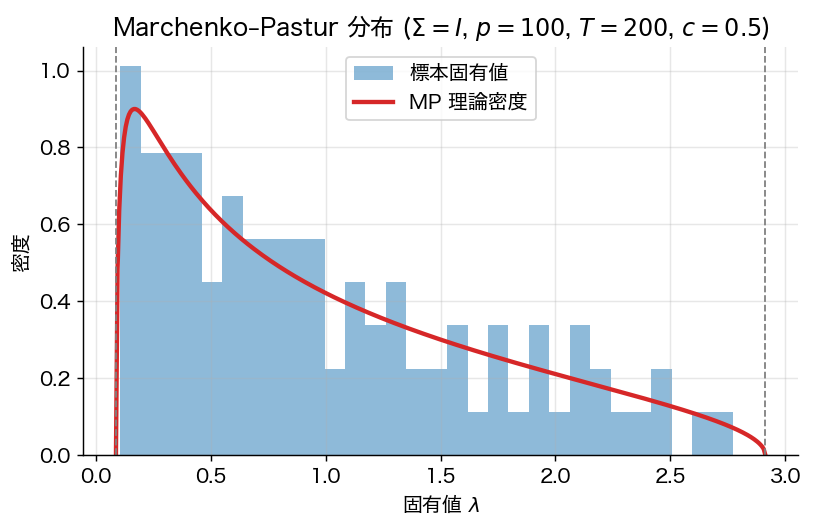
\includegraphics[width=0.85\linewidth]{figures/marchenko_pastur.png}
\caption{Marchenko-Pastur 分布（理論曲線）と標本固有値ヒストグラム。$\Sigma=I$ にも関わらず標本固有値は広く分布し、特に最小固有値はゼロ近傍に張り付く — これが Markowitz 最適化を不安定にする。}
\end{figure}

\section{12.2 線形縮小推定（Ledoit–Wolf 2004）}

\textbf{戦略}：$S$ と「単純な目標行列」$F$ の凸結合 \[ \hat\Sigma^{\rm LW}(\alpha) = (1 - \alpha)\, S + \alpha\, F, \qquad \alpha \in [0, 1] \] を取り、$\alpha$ を最適化する。原典では $F = \mu I_p$、$\mu = \mathrm{tr}(\Sigma)/p$（平均固有値の倍数）。

\textbf{定理 12.2}（Ledoit–Wolf 2004、JMVA 88: 365–411） Frobenius ノルム損失 \[ L(\alpha) = \mathbb{E}\bigl[ \| \hat\Sigma^{\rm LW}(\alpha) - \Sigma \|_F^2 \bigr] \] を最小化する \textbf{oracle 最適縮小強度} は \[ \alpha^\star = \frac{\sum_{i,j} \mathrm{Var}(S_{ij})}{\sum_{i,j} \mathrm{Var}(S_{ij}) + \| \Sigma - \mu I \|_F^2}. \] 標本から推定可能な $\hat\alpha$ が $\alpha^\star$ に大次元漸近 $p/T \to c \in (0,\infty)$ で一致する。

\emph{証明方針}：
\begin{itemize}
\item 損失を展開 $L(\alpha) = \alpha^2 \|S - \mu I - (S - F)\text{(deterministic)}\|^2$ 等の項に分解。
\item バイアス–分散分解より $L(\alpha) = (1-\alpha)^2 \cdot \mathrm{Var}\text{項} + \alpha^2 \cdot \mathrm{Bias}\text{項}$。
\item 一階条件から $\alpha^\star$。
\item 4次モーメントから $\sum \mathrm{Var}(S_{ij})$ を一致推定。$\square$
\end{itemize}

\textbf{重要 caveat}（査読者目線）：
\begin{itemize}
\item 大次元漸近では $\hat\Sigma^{\rm LW}$ は \textbf{真の $\Sigma$ の各成分} に一致しない。一致するのは \textbf{oracle 縮小強度} $\alpha^\star$。
\item $F = \mu I$ は等方目標、より sophisticated な目標（定数相関、因子モデル）も使える。
\end{itemize}

\section{12.3 非線形縮小（概観のみ）}

線形縮小は全固有値を一様に縮小する。\textbf{非線形縮小}（Ledoit–Wolf 2012）は \textbf{各固有値を個別に処理} する。直観は次の通り：

\begin{itemize}
\item 大固有値（市場・主要因子の方向）は \textbf{そのまま} 残す
\item 小固有値（ノイズで膨らんだ方向）は \textbf{大きく} 縮小する
\item 中間は連続的に補間
\end{itemize}

このような「固有値ごとの最適補正」は \textbf{ランダム行列理論（Random Matrix Theory; RMT）} で導かれる。Bun–Bouchaud–Potters (2017, \emph{Physics Reports} 666: 1–109) は物理学コミュニティで「相関行列のクリーニング」として独立に同じアイデアを発展させた。

学部レベルでは「\textbf{線形縮小（Ledoit–Wolf 2004）が実装でほぼ標準}」と覚えておけばよい。非線形版の数式は専門書（章末道標）に進んだときに学べばよい。

\section{12.4 因子モデルベースの縮小}

ファクター構造 $\Sigma = B \Omega B^\top + D$ を仮定するなら、推定パラメタ数が $\mathcal{O}(p^2)$ から $\mathcal{O}(pK)$ に減る（第5章 5.5 節）。これは Fama–French 等の経済理論をもつ \textbf{構造的縮小} と解釈できる。Ledoit–Wolf の \textbf{constant correlation} 目標 \[ F_{ij} = \begin{cases} s_{ii} & i = j \\ \bar\rho \cdot \sqrt{s_{ii} s_{jj}} & i \neq j \end{cases} \] （$\bar\rho$ は平均標本相関）も実用上効果的（Ledoit–Wolf 2003, "Improved Estimation of the Covariance Matrix of Stock Returns"）。

\section{12.5 Minimum Variance Portfolio への効果}

GMV ポートフォリオ $w^{\rm GMV} = \Sigma^{-1} \mathbf{1} / (\mathbf{1}^\top \Sigma^{-1} \mathbf{1})$ について、$S$ で代用すると out-of-sample 分散が著しく増加する。Ledoit–Wolf 縮小は、極端なロングショート（$|w_i|$ が大きい）を抑制し、out-of-sample で \textbf{より低い実現分散} を達成することが繰り返し実証されている（DeMiguel–Garlappi–Uppal 2009, \emph{RFS} 22: 1915–1953）。

\textbf{実証的事実}：1/N ナイーブ等加重と Markowitz（$S$ 推定）を比較すると、多くの実証で \textbf{1/N が勝つ}。Ledoit–Wolf 縮小を使った Markowitz は 1/N と互角〜やや優位。これが「単純なものほど頑健」という Markowitz の実装上の困難を端的に示す。

\begin{figure}[H]
\centering
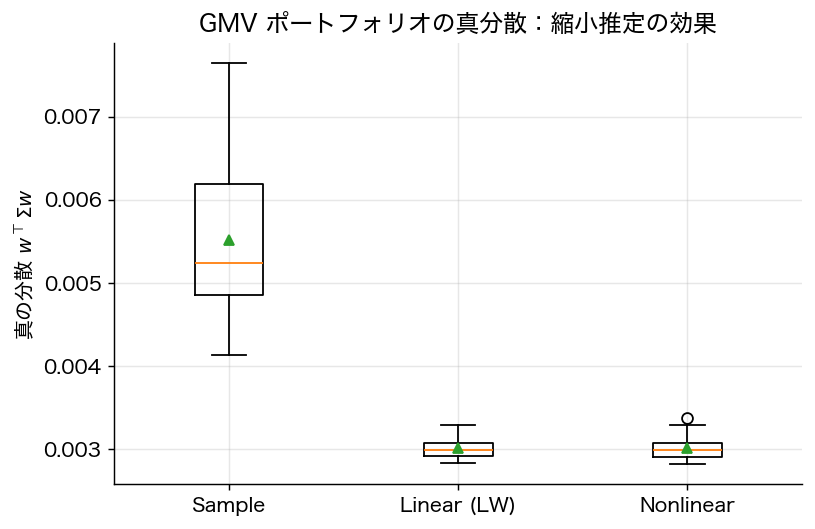
\includegraphics[width=0.85\linewidth]{figures/shrinkage_compare.png}
\caption{共分散推定法の効果比較：標本共分散・線形縮小・非線形縮小それぞれを使った GMV の out-of-sample 分散。データ駆動の縮小は安定性を改善する。}
\end{figure}

\section{12.6 実装の要点}

```python
\chapter{Ledoit-Wolf 線形縮小（scikit-learn 実装）}
from sklearn.covariance import LedoitWolf lw = LedoitWolf().fit(returns) Sigma\_hat = lw.covariance\_ alpha\_hat = lw.shrinkage\_  \# 推定された縮小強度 ```

\section{12.7 まとめ}

\begin{itemize}
\item 大次元下で標本共分散は固有値分布が病的に広がる（Marčenko–Pastur）。
\item 線形縮小は \textbf{oracle 縮小強度} を一致推定する強力な手法。
\item 非線形縮小は各固有値を個別最適化、RMT cleaning と等価。
\item 因子モデルは経済理論をもつ構造的縮小として捉えられる。
\item 1/N ナイーブと比べた優位性は実証データに依存し、\textbf{縮小を入れないと負ける} ことが多い。
\end{itemize}

\begin{quote}
🛣 \textbf{上級学習への道標}
- \textbf{Marčenko–Pastur 分布の Stieltjes 変換による導出} と非線形縮小の閉形式：Bun–Bouchaud–Potters \emph{Cleaning Large Correlation Matrices: Tools from Random Matrix Theory}, Physics Reports 666 (2017)。
- \textbf{自由確率論（free probability）と S-変換}：行列値確率変数の足し算・掛け算の極限分布を扱う数学的枠組み（Voiculescu）。
- \textbf{非線形縮小の実装}：QuEST 法 (Ledoit–Wolf 2017, \emph{Annals of Statistics} 45: 3175–3198)、Direct kernel 法 (Ledoit–Wolf 2020)。
\end{quote}

\noindent\hrulefill

% ===== 13_robust_optimization.md =====
\chapter{第13章 ロバスト/分布ロバスト・ポートフォリオ最適化}

\begin{quote}
🎯 \textbf{この章で答える問い}
- 「期待リターン $\mu$ が \textbf{本当には} いくらか分からない」状態でどう最適化するか。
- \textbf{min–max（最悪ケース）} 最適化のアイデアと、それが Markowitz 解とどう違うか。
- 「ロバストにする = 分散する」ではない、という驚くべき事実。

📐 \textbf{使う数学}：ラグランジュ法、Cauchy–Schwarz 不等式。

⚠️ \textbf{本章の方針}：SOCP/SDP の \textbf{凸最適化の詳細} や \textbf{Wasserstein 距離} は学部 4 年向けには重い。本書では「不確実性集合の半径 $\kappa$ を変えるとフロンティアがどう動くか」という直観中心で解説する。
\end{quote}

Markowitz 解は $\mu, \Sigma$ の推定誤差に対して \textbf{極端に高感度} であった（第1章 1.7 節）。本章では「パラメタが不確実性集合に属することのみ仮定」して \textbf{最悪ケース最適化} を行うフレームワークを展開する。

\section{13.1 楕円体不確実性集合（Goldfarb–Iyengar 2003）}

\textbf{問題}：期待リターンが点推定 $\hat\mu$ の周りの楕円体に属し \[ \mathcal{U}_\mu = \{ \mu : (\mu - \hat\mu)^\top \Theta^{-1} (\mu - \hat\mu) \le \kappa^2 \}. \] 共分散 $\Sigma$ も因子構造 $\Sigma = B \Omega B^\top + D$ に基づく不確実性集合 $\mathcal{U}_\Sigma$ に属するとする。

\textbf{目標}：分散制約下で最悪ケース期待リターンを最大化 \[ \max_w\ \min_{\mu \in \mathcal{U}_\mu}\ w^\top \mu \quad \text{s.t.}\quad \max_{\Sigma \in \mathcal{U}_\Sigma} w^\top \Sigma w \le \sigma_0^2,\ \mathbf{1}^\top w = 1. \]

\textbf{定理 13.1}（Goldfarb–Iyengar 2003, \emph{Math. Oper. Res.} 28: 1–38） 上記問題は \textbf{二次錐計画（SOCP）} に等価変換され、効率的に解ける： \[ \max_w\ w^\top \hat\mu - \kappa \|\Theta^{1/2} w\|_2,\quad \text{s.t.}\ \cdots \]

\emph{証明方針}：
\begin{itemize}
\item 内側 min は楕円体内の双対化により $\min_\mu w^\top \mu = w^\top \hat\mu - \kappa \sqrt{w^\top \Theta w}$（Cauchy–Schwarz）。
\item 共分散の不確実性は半正定値性を保ったまま LMI 制約に書き直せる。
\item 全体として SOCP / SDP に帰着。$\square$
\end{itemize}

\textbf{実装ヒント}：CVXPY などのコーン最適化ソルバで実装可能。$\kappa$ は \textbf{信頼度パラメタ}（$\kappa = \chi^2_p(1-\delta)^{1/2}$ で $1-\delta$ 信頼集合に対応）。

\section{13.2 査読者の警告：robust ≠ 分散}

「Goldfarb–Iyengar が SOCP に落ちる」ことと「結果がよいポートフォリオ」であることは別。\textbf{不確実性集合の半径・形状} に結果が極端に依存する：

\begin{itemize}
\item $\kappa$ を大きく取りすぎると過度に保守的、低リターン資産・少数資産への偏り。
\item $\kappa$ を小さく取ると古典 Markowitz と差が出ない。
\item separable な楕円体は非分散的になりやすい（Lu 2011, \emph{Math. Programming} 126: 193–201）。
\end{itemize}

教育上の重要メッセージ：\textbf{robust 最適化 = 分散投資ではない}。

\section{13.3 Garlappi–Uppal–Wang のアプローチ（2007）}

\textbf{Garlappi–Uppal–Wang 2007}（\emph{RFS} 20: 41–81）は Bayesian/multi-prior 枠組みで \textbf{閉形式} の robust 解を導く。

\textbf{設定}：投資家は $\mu$ について事前 $\mu \sim \mathcal{N}(\hat\mu, \Sigma/\tau)$（推定誤差を反映）を持ち、各 prior 集合上で \textbf{max–min 期待効用} \[ \max_w \min_{\mu \in \mathcal{P}_\delta(\hat\mu)} \mathbb{E}[U(W)] \] を解く。$\mathcal{P}_\delta$ は likelihood ratio 制約による「曖昧性集合」。

\textbf{主結果}：最適解は \textbf{古典 Markowitz 解の縮小}： \[ w_{\rm GUW}^\star = \frac{1}{\gamma + \epsilon(\delta, \tau)}\, \Sigma^{-1}(\hat\mu - r_f \mathbf{1}) \] （$\epsilon$ は曖昧性度・標本誤差から決まる罰金項）。すなわち \textbf{曖昧性回避} は古典解を「無リスク資産方向」または「最小分散ポートフォリオ方向」へシフトさせる。

\textbf{驚くべき含意}：
\begin{itemize}
\item 曖昧性集合の置き方によっては \textbf{市場不参加（non-participation）} が最適となる。
\item これは「分散投資が必ず良い」という Markowitz の直観と相容れない。
\item 実証的にエクイティ・プレミアム・パズルや home bias の説明候補となる。
\end{itemize}

\section{13.4 分布ロバスト最適化（DRO、概観のみ）}

近年の発展は \textbf{分布ロバスト最適化（Distributionally Robust Optimization; DRO）}。これは「真の分布 $P$ が未知だが、経験分布 $\hat P_T$ の \textbf{近所} にあると仮定」する枠組みで、最悪ケース期待損失を最小化する： \[ \min_w \sup_{P \in \mathcal{P}_\rho(\hat P_T)} \mathbb{E}_P[L(w, R)]. \]

不確実性集合 $\mathcal{P}_\rho$ の作り方で大きく 2 種類：

\begin{enumerate}
\item \textbf{モーメント DRO}（Delage–Ye 2010）：平均・共分散だけ信頼区間で抑える。
\item \textbf{Wasserstein DRO}（Mohajerin Esfahani–Kuhn 2018）：経験分布から確率質量を「動かすコスト」が $\rho$ 以下の分布族。
\end{enumerate}

\textbf{重要な結果（驚き）}：Wasserstein DRO は \textbf{「経験平均 + 正則化項」} の形に書き直せ、これが \textbf{L2 正則化や Lasso と等価} になる場合がある。すなわち \textbf{ロバスト最適化と機械学習の正則化は同じコインの両面} という驚くべき洞察を生んだ。

学部レベルでは「DRO は『分布が分からない状況で最悪ケース最適化する技術』であり、機械学習の正則化と深い関係がある」と理解しておけば十分。詳細な数式は章末の道標を参照。

\section{13.5 数値例：Robust frontier}

楕円体不確実性 $\kappa = 0.5, 1.0, 1.5$ のフロンティアを描くと、$\kappa$ が大きいほどフロンティアが下方シフト（より保守的）。古典 Markowitz フロンティアは $\kappa = 0$ に対応。

\begin{figure}[H]
\centering
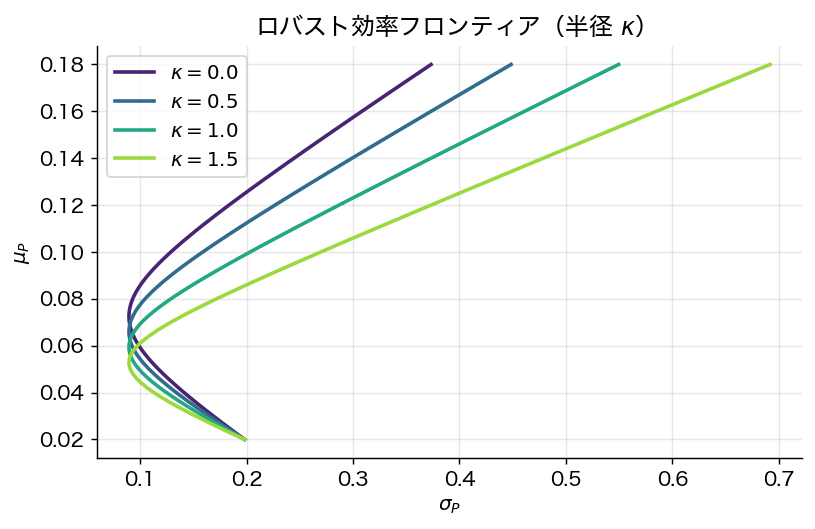
\includegraphics[width=0.85\linewidth]{figures/robust_frontier.png}
\caption{ロバスト最適化の効果：楕円体不確実性の半径 $\kappa$ を変えたフロンティアの比較。古典フロンティアと、不確実性を考慮した frontier が異なる位置に来る。}
\end{figure}

\section{13.6 まとめ}

\begin{itemize}
\item ロバスト最適化は推定誤差を \textbf{明示的に} モデル化。
\item Goldfarb–Iyengar の楕円体 SOCP はクリーンだが、集合設計次第で非分散になりうる。
\item Garlappi–Uppal–Wang の閉形式は古典解の縮小として解釈でき、曖昧性回避が \textbf{市場不参加} すら導きうる。
\item Delage–Ye と Wasserstein DRO は機械学習との橋渡し。
\item 「robust = 分散 = 安定」は誤った直観：パラメタ設計が結果を支配する。
\end{itemize}

\begin{quote}
🛣 \textbf{上級学習への道標}
- \textbf{凸最適化と SOCP/SDP}：Boyd \& Vandenberghe \emph{Convex Optimization} (2004)、Ben-Tal–El Ghaoui–Nemirovski \emph{Robust Optimization} (2009)。
- \textbf{Wasserstein DRO の数式}：Mohajerin Esfahani \& Kuhn (2018) は経験分布の確率質量を「動かすコスト」を Wasserstein 距離（最適輸送理論の距離）で測る。これが正則化機械学習と等価になる議論は Blanchet–Murthy (2019), Sinha–Namkoong–Duchi (2018) を参照。
- \textbf{CVaR と DRO の関係}：CVaR は実は「ある特定の Wasserstein 不確実性集合上の DRO」として再解釈できる。
\end{quote}

\noindent\hrulefill

% ===== 14_risk_parity_hrp.md =====
\chapter{第14章 リスクパリティと階層的リスクパリティ（HRP）}

Markowitz 流の平均分散最適化は期待リターン $\mu$ の推定誤差に致命的に弱い。\textbf{リスクパリティ} は期待リターンを完全に放棄し、\textbf{リスク寄与の均等化} だけを基準とする。

\section{14.1 リスク寄与の定義}

ポートフォリオ全体の標準偏差 $\sigma_P(w) = \sqrt{w^\top \Sigma w}$ は資産重み $w$ の \textbf{1 次同次} 関数。Euler の定理から \[ \sigma_P(w) = \sum_i w_i \cdot \frac{\partial \sigma_P}{\partial w_i}. \]

\textbf{定義 14.1}（限界リスク寄与・リスク寄与） \[ \mathrm{MRC}_i := \frac{\partial \sigma_P}{\partial w_i} = \frac{(\Sigma w)_i}{\sqrt{w^\top \Sigma w}},\qquad \mathrm{RC}_i := w_i \cdot \mathrm{MRC}_i = \frac{w_i (\Sigma w)_i}{\sigma_P(w)}. \] $\sum_i \mathrm{RC}_i = \sigma_P(w)$（Euler 分解）が成立。

\section{14.2 Equal Risk Contribution（ERC）}

\textbf{定義 14.2}（ERC ポートフォリオ） 全資産のリスク寄与が等しい： \[ \mathrm{RC}_i = \frac{\sigma_P(w)}{n}, \quad i = 1, \dots, n. \] あるいは等価に $w_i (\Sigma w)_i = w_j (\Sigma w)_j$ for all $i, j$。

\subsection{14.2.1 対角共分散の場合}

$\Sigma = \mathrm{diag}(\sigma_1^2, \dots, \sigma_n^2)$ なら $\mathrm{RC}_i \propto w_i^2 \sigma_i^2$。等寄与条件 $w_i \sigma_i = $ const から \[ \boxed{\; w_i^{\rm ERC} = \frac{1/\sigma_i}{\sum_j 1/\sigma_j} \quad (\sigma_i \text{ は標準偏差}) \;} \]

\textbf{注}：$\sigma_i$ を \textbf{分散} と呼ぶ書物もあるので注意。本書では一貫して $\sigma_i$ は標準偏差。

\subsection{14.2.2 二資産の場合}

相関 $\rho$ の二資産では、ERC 解は驚くべきことに \textbf{相関に依存しない}： \[ w_1^{\rm ERC} = \frac{\sigma_2}{\sigma_1 + \sigma_2}, \quad w_2^{\rm ERC} = \frac{\sigma_1}{\sigma_1 + \sigma_2}. \]

\emph{証明方針}：等寄与条件 $w_1 (\Sigma w)_1 = w_2 (\Sigma w)_2$ を展開し、$\rho \sigma_1 \sigma_2 w_1 w_2$ 項が両辺に現れて相殺。$\square$

\subsection{14.2.3 一般 $\Sigma$：存在性と一意性}

\textbf{定理 14.3}（Maillard–Roncalli–Teiletche 2010, \emph{JPM} 36(4): 60–70） $\Sigma \succ 0$ かつ長オンリー（$w > 0$）制約下で、ERC ポートフォリオは存在し一意に決まる。

\emph{証明方針}（Bai–Scheinberg–Tütüncü 2016, \emph{J. Optim. Theory Appl.} 168: 1–28）：
\begin{itemize}
\item 凸プログラム
\end{itemize}
\[ \min_{y > 0} \frac{1}{2} y^\top \Sigma y - \sum_i \log y_i \] を解くと最適 $y^\star$ から $w_i^{\rm ERC} = y_i^\star / \sum_j y_j^\star$。
\begin{itemize}
\item 目的関数は強凸（$-\sum \log y_i$ は強凸、$\Sigma \succ 0$）。
\item 一階条件 $\Sigma y = \mathrm{diag}(1/y_1, \dots, 1/y_n) \mathbf{1}$ より $y_i (\Sigma y)_i = 1$、正規化して ERC 条件と一致。$\square$
\end{itemize}

\textbf{caveat}：ショート可・特異 $\Sigma$・追加制約付きでは一意性が崩れる。

\section{14.3 リスクパリティの実証性質}

Asness–Frazzini–Pedersen 2012（\emph{Financial Analysts Journal} 68: 47–59）は「low-risk anomaly + レバレッジ回避」によりリスクパリティが Sharpe を改善することを示した。実務的に Bridgewater の All Weather や AQR の Risk Parity Fund などが採用。

\textbf{ただし}：
\begin{itemize}
\item リスクパリティはレバレッジを要する（債券側にレバ）→ 借入金利・流動性リスク。
\item 「リスクが均等」≠「真に分散」。例えば全資産が高相関ならリスク寄与が均等でも単一因子に集中。
\item 2008・2020 の市場ストレスでは相関上昇により分散効果が失われた。
\end{itemize}

\section{14.4 階層的リスクパリティ（HRP, López de Prado 2016）}

López de Prado 2016（\emph{JPM} 42(4): 59–69）は標本共分散の特異性問題を回避する三段階アルゴリズム HRP を提案。

\subsection{14.4.1 アルゴリズム}

\textbf{Step 1: Tree clustering} 相関行列 $C$ から \textbf{距離行列} \[ d_{ij} = \sqrt{\frac{1 - C_{ij}}{2}} \in [0, 1] \] を作る。$d$ は metric（三角不等式を満たす、Mantegna 1999）。階層クラスタリング（典型的に \textbf{single linkage}）でデンドログラムを構築。

\textbf{Step 2: Quasi-diagonalization} クラスタの順序で資産を並び替え、相関行列をブロック対角に近づける。$\Sigma$ そのものは触らないが、後段の bisection 順序を決める。

\textbf{Step 3: Recursive bisection} 全資産に重み 1 を初期化、並び替え順序のリストを再帰的に二分割：

``\texttt{ function HRP\textbackslash{}\_alloc(weights, items): if len(items) == 1: return L, R = split items in half σ²\textbackslash{}\_L = v\textbackslash{}\_L\textbackslash{}textasciicircum\{\}T Σ\textbackslash{}\_L v\textbackslash{}\_L  where v\textbackslash{}\_L\textbackslash{}\_i ∝ 1/Σ\textbackslash{}\_ii σ²\textbackslash{}\_R = v\textbackslash{}\_R\textbackslash{}textasciicircum\{\}T Σ\textbackslash{}\_R v\textbackslash{}\_R  where v\textbackslash{}\_R\textbackslash{}\_i ∝ 1/Σ\textbackslash{}\_ii α = σ²\textbackslash{}\_R / (σ²\textbackslash{}\_L + σ²\textbackslash{}\_R) weights[L] \emph{= α weights[R] }= (1 - α) HRP\textbackslash{}\_alloc(weights, L) HRP\textbackslash{}\_alloc(weights, R) }``

各ステップで二資産問題 $\min_\alpha \alpha^2 \sigma_L^2 + (1-\alpha)^2 \sigma_R^2$ の最小化（解 $\alpha = \sigma_R^2/(\sigma_L^2 + \sigma_R^2)$）として導出される。

\subsection{14.4.2 HRP の利点（López de Prado の主張）}

\begin{itemize}
\item \textbf{$\Sigma^{-1}$ を使わない} → 特異・悪条件共分散に頑健。
\item 階層構造が経済的にも意味を持つ（業界クラスタ等）。
\item 計算量 $\mathcal{O}(n \log n)$ で大規模問題に向く。
\end{itemize}

\subsection{14.4.3 査読者の警告：HRP は本当に out-of-sample で勝つのか}

López de Prado 2016 の優位主張は主に Monte Carlo に依存し、実データでの普遍的優位は確立されていない。

\begin{itemize}
\item \textbf{Jain–Jain (2019)}: 粗い共分散推定では inverse-volatility が最も頑健、HRP は中間的。HRP が常に勝つわけではない。
\item \textbf{Pfitzinger–Katzke (2019)}: HRP の弱点を補う Constrained HRP (CHRP) を提案。素の HRP に実務上の不足があることを暗黙に認める。
\item \textbf{比較対象の脆弱性}：CLA（Critical Line Algorithm）と HRP の比較で CLA は標本共分散を直接使う最弱の Markowitz。LW 縮小入りの GMV や ERC との比較ではないため、優位性の主張は割り引いて読むべき。
\end{itemize}

\textbf{結論}：HRP は「便利な heuristic」として教えるべきで、厳密な最適性主張はしない。

\begin{figure}[H]
\centering
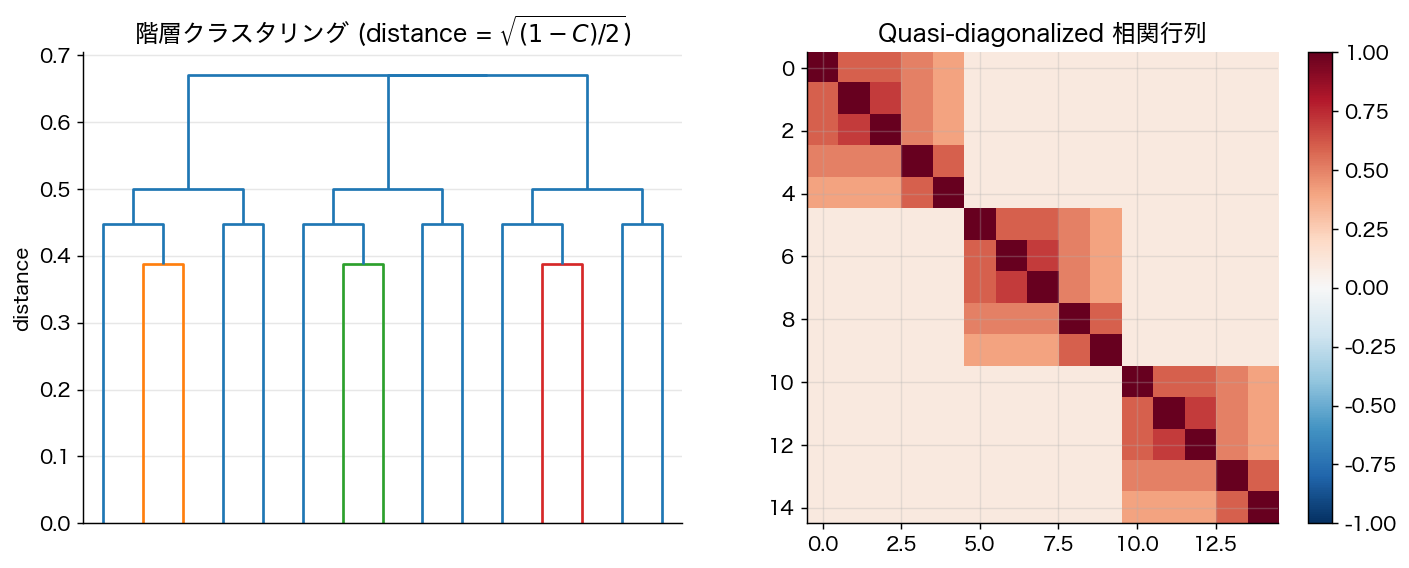
\includegraphics[width=0.85\linewidth]{figures/hrp_dendrogram.png}
\caption{階層的リスクパリティ：相関ベース距離からの階層クラスタリング（デンドログラム）と quasi-diagonalized 相関行列。再帰的二分割によりウェイトを配分する。}
\end{figure}

\section{14.5 ERC vs Markowitz vs HRP}

実証上の経験則（DeMiguel–Garlappi–Uppal 2009 以来）：

\begin{center}
\begin{tabular}{|l|l|l|l|l|}
\hline
手法 & $\mu$ 推定 & $\Sigma$ 推定 & 必要レバ & OOS Sharpe \\ \hline
1/N & 不要 & 不要 & なし & 高い（驚くほど） \\ \hline
Markowitz（$S$） & 重要 & 重要 & 大 & 不安定 \\ \hline
GMV（$S$） & 不要 & 重要 & 中 & 不安定 \\ \hline
GMV + LW 縮小 & 不要 & 軽減 & 中 & 良好 \\ \hline
ERC & 不要 & 軽 & 中 & 良好 \\ \hline
HRP & 不要 & 軽 & 中 & 良好だが状況依存 \\ \hline
\end{tabular}
\end{center}

実証上、$\mu$ 推定を必要としない手法群（GMV、ERC、HRP）が比較的安定。Markowitz そのものは縮小推定なしには「実装するな」とまで言われる（Michaud 1989, "Markowitz Optimization Enigma"）。

\section{14.6 まとめ}

\begin{itemize}
\item ERC はリスク寄与均等化で、対角 $\Sigma$ では $w \propto 1/\sigma$。二資産では相関に依存しない。
\item 一般の ERC は凸プログラム $\min_y \tfrac{1}{2} y^\top \Sigma y - \sum \log y_i$ の最適化に等価。
\item HRP は階層クラスタリング + 再帰的二分割の heuristic。$\Sigma^{-1}$ を避けるが、共分散・距離・linkage への依存性は残る。
\item HRP の OOS 優位性は contested。教えるなら caveat 付きで。
\item 実証上は「$\mu$ 推定を必要としない」手法群が一般に安定。
\end{itemize}

\noindent\hrulefill

% ===== 15_factor_zoo_ml.md =====
\chapter{第15章 ファクター動物園・FF5・q ファクター・機械学習資産価格}

第5章で Fama–French 3 因子と Carhart 4 因子モデルを導入したが、2010 年以降この分野は \textbf{多重検定の認識} と \textbf{機械学習の流入} で大きく変容した。

\section{15.1 Fama–French 5 因子モデル（FF5）}

Fama–French 2015（\emph{JFE} 116(1): 1–22）は HML, SMB に加え \textbf{収益性（RMW: Robust Minus Weak）} と \textbf{投資保守度（CMA: Conservative Minus Aggressive）} の二因子を追加。

\[ R_i - r_f = \alpha_i + b_i \cdot \mathrm{MKT} + s_i \cdot \mathrm{SMB} + h_i \cdot \mathrm{HML} + r_i \cdot \mathrm{RMW} + c_i \cdot \mathrm{CMA} + \varepsilon_i. \]

\textbf{理論的根拠}：配当割引モデルの恒等式 \[ \frac{P_t}{B_t} = \frac{\sum_\tau \mathbb{E}_t[\text{利益}_{t+\tau}]/(1 + r)^\tau}{B_t} \] を整理すると、期待リターン $r$ は \textbf{B/M, 期待利益、期待投資成長率} の関数になる。これが「価値・収益性・投資」の三因子論を動機付ける。

\textbf{Fama–French 自身が認めた弱点}：
\begin{enumerate}
\item \textbf{HML の冗長性}：FF5 内では HML が RMW と CMA に説明される。価値ファクターの「勝利」ではなく「吸収」。
\item \textbf{モメンタムの未説明}：FF5 もモメンタムを説明できない。Fama–French 2016（\emph{RFS} 29: 69–103）は FF6（モメンタム追加版）を後に提案。
\item \textbf{小型成長株の異常リターン}：低収益・積極投資の小型株の低リターンを捕まえきれない。
\end{enumerate}

\section{15.2 Hou–Xue–Zhang の q ファクターモデル}

Hou–Xue–Zhang 2015（\emph{RFS} 28: 650–705）は投資理論（Tobin's q）から導出された 4 因子モデル：

\begin{itemize}
\item $\mathrm{R}_{MKT}$: 市場
\item $\mathrm{R}_{ME}$: サイズ（FF SMB に対応）
\item $\mathrm{R}_{IA}$: 投資（CMA に近い）
\item $\mathrm{R}_{ROE}$: 収益性（RMW に近い）
\end{itemize}

\textbf{Hou–Mo–Xue–Zhang 2019（\emph{Review of Finance} 23: 1–35）の結論}：q ファクターは FF5/FF6 の主要なアノマリを \textbf{spanning test} で吸収する。すなわち q ファクターを所与とすると、FF5 因子（HML, CMA, RMW）の超過リターンは大半消える。

\textbf{q5 モデル}（Hou et al. 2021, \emph{Review of Finance} 25: 1–41）：q ファクターに \textbf{expected growth} を追加し、FF6 を上回ると主張。

\textbf{現代の状況}：「FF5 が決着済み標準」ではない。FF5、FF6、q-factor、q5 が競合する。実証選択はデータ・期間・サンプルセレクションに依存。

\begin{figure}[H]
\centering
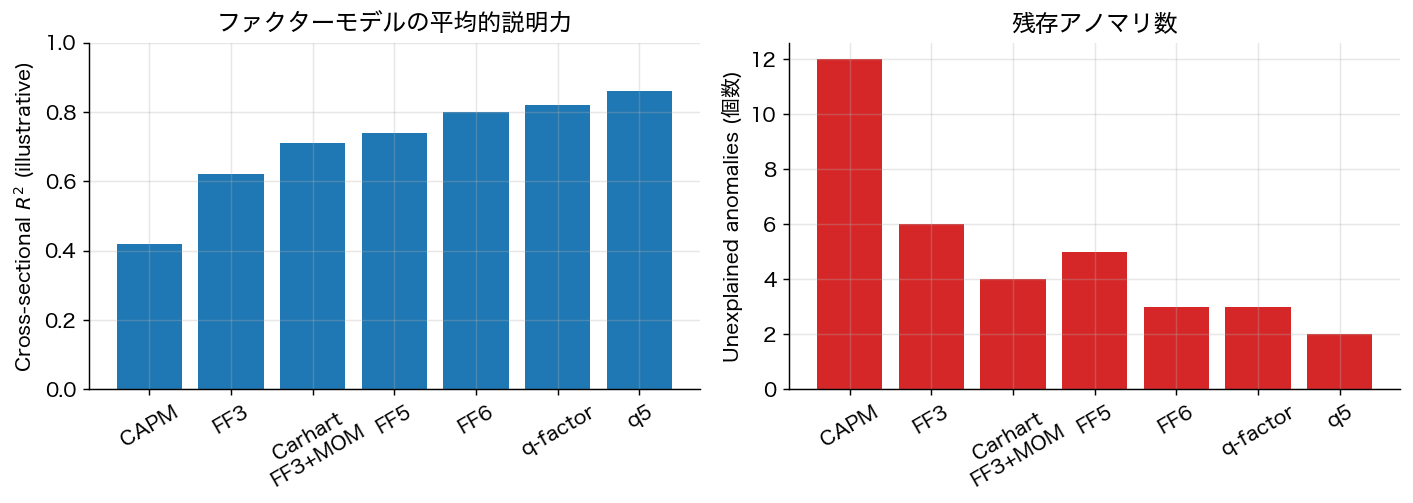
\includegraphics[width=0.85\linewidth]{figures/factor_models_compare.png}
\caption{FF5・FF6・q ファクターモデルの spanning test 結果の比較。各モデルが他モデルの因子をどれだけ説明（subsume）するか。}
\end{figure}

\section{15.3 ファクター動物園と多重検定}

Cochrane 2011（AFA Presidential Address, \emph{Journal of Finance} 66: 1047–1108）の問題提起：\textbf{「factor zoo」} — 数百本の "新発見" アノマリが論文として publish されている。

\subsection{15.3.1 Harvey–Liu–Zhu の警告}

Harvey–Liu–Zhu 2016（\emph{RFS} 29: 5–68）は 1967–2014 年に提案された \textbf{316 ファクター} をカタログ化し、多重検定補正後に「真に有意」と言えるものは少数だと示した。

\textbf{主張}：従来「$t > 2$」を有意の閾値としてきたが、多重検定下では正しくない。
\begin{itemize}
\item \textbf{Bonferroni 補正}：$N$ テストなら $|t| > \Phi^{-1}(1 - \alpha/(2N))$。$N = 316$, $\alpha = 0.05$ なら $|t| > 3.39$。
\item \textbf{Holm 法}：順序付き $p$ 値に対する漸近的補正。
\item \textbf{Benjamini–Hochberg（FDR 法）}：False Discovery Rate を制御。
\end{itemize}

ファクターの大多数は $|t| < 3$ で、多重検定後は \textbf{生き残らない}。

\subsection{15.3.2 Feng–Giglio–Xiu（2020）の "Taming the Factor Zoo"}

Feng–Giglio–Xiu 2020（\emph{JF} 75: 1327–1370）は機械学習（\textbf{double machine learning}）で「真に新規な」ファクターを発見する手続きを提案。手順：

\begin{enumerate}
\item 既存 $K$ ファクターと候補新規ファクターを所与とする。
\item SDF（確率割引因子）の推定に既存ファクターを反映。
\item 新規ファクターの \textbf{増分} 寄与を Lasso 等で評価。
\item 多重検定補正下で増分有意なものだけ採用。
\end{enumerate}

結果：多くの「新発見」は既存ファクターに吸収され、真に独立な新規因子は少数（10 個前後）。

\section{15.4 機械学習資産価格}

\subsection{15.4.1 Gu–Kelly–Xiu（2020）：ML が古典モデルを凌駕}

Gu–Kelly–Xiu 2020（\emph{RFS} 33: 2223–2273）は数百の firm characteristics から多様な ML 手法（ニューラルネット、勾配ブースティング、ランダムフォレスト、Lasso）で月次リターンを予測。

\textbf{結果}：
\begin{itemize}
\item ニューラルネット（2–5 層）が最高性能、R\textasciicircum{}2 が線形モデル比 2–4 倍。
\item 価値・モメンタムだけでなく、リターン予測において \textbf{流動性・取引摩擦・短期反転} が重要。
\item 経済的に大きい長短ロング・ショート Sharpe（年率 2.5–3.0 程度）。
\end{itemize}

\textbf{重要 caveat}：
\begin{itemize}
\item 取引コスト・空売り制約・規模効果を考慮するとずっと小さくなる。
\item 統計的予測力と取引可能な戦略は別。
\end{itemize}

\subsection{15.4.2 Kelly–Pruitt–Su（2019）：Instrumented PCA（IPCA）}

Kelly–Pruitt–Su 2019（\emph{JFE} 134: 501–524）は \textbf{特性（characteristics）が因子負荷量に直接対応} する条件付き因子モデル： \[ R_{i,t+1} = \beta_{i,t} \cdot f_{t+1} + \varepsilon_{i,t+1}, \qquad \beta_{i,t} = Z_{i,t} \Gamma + u_{i,t} \] （$Z_{i,t}$ は firm characteristics、$\Gamma$ は推定する負荷写像）。

これは「特性は β を時変させる」という形での \textbf{特性 = 共分散} 仮説。少数の因子（5–6 個）で多数のアノマリを説明することに成功。

\subsection{15.4.3 Chen–Pelger–Zhu（2023）：Deep Learning + No-Arbitrage}

Chen–Pelger–Zhu 2023（\emph{Management Science} 70: 714–750）は \textbf{無裁定条件をニューラルネットに損失として組み込む}： \[ \mathcal{L} = \sum_t \| \mathbb{E}_t[M_{t+1} R_{t+1}] - 1 \|^2 + \lambda \cdot \mathrm{NN\text{-}penalty}. \] これは APT を ML の枠組みで再構成した試み。

\section{15.5 ML 資産価格の落とし穴}

\begin{itemize}
\item \textbf{データスヌーピング}：何百もの特性から探したものは selection bias を含む。
\item \textbf{構造変化（regime shift）}：訓練期間と異なる時期は予測力低下。
\item \textbf{取引コスト}：高頻度回転戦略は実装困難。
\item \textbf{解釈可能性}：ニューラルネット予測は経済的解釈が困難。SHAP/特徴量重要度等で部分的に分析可。
\item \textbf{再現性}：データ前処理・サンプル選択・特性の定義が論文間で異なる。
\end{itemize}

\section{15.6 まとめ}

\begin{itemize}
\item FF5 は HML の冗長性とモメンタム未説明を内包。FF6 でも完全ではない。
\item q ファクター（Hou–Xue–Zhang）は FF5 と競合。q5 で expected growth を追加。
\item 数百のアノマリから「真に独立な」因子は数十個程度（Harvey–Liu–Zhu、Feng–Giglio–Xiu）。
\item 多重検定補正が現代資産価格論の必須要件。
\item 機械学習は予測力を向上させるが、取引可能性・解釈可能性・再現性に課題。
\end{itemize}

\noindent\hrulefill

% ===== 16_backtest_overfit.md =====
\chapter{第16章 バックテスト過剰適合と Deflated Sharpe 比}

第11章では Sharpe 比とその統計的検出力を扱った。本章では \textbf{複数戦略を比較した上で最良を選ぶ} という、実務でほぼ普遍的な状況下での評価バイアスを定量化する。

\section{16.1 問題：選択バイアス}

$N$ 個の独立戦略 $\{s_1, \dots, s_N\}$ から事後最良 $s^\star = \arg\max_i \widehat{\mathrm{SR}}_i$ を選ぶ。$s^\star$ の標本 Sharpe は \textbf{過大評価} される。

\textbf{極値理論からの近似}：$\widehat{\mathrm{SR}}_i \sim_{\rm iid} \mathcal{N}(0, \sigma_{\rm SR}^2)$ なら \[ \mathbb{E}[\max_{i=1, \dots, N} \widehat{\mathrm{SR}}_i] \approx \sigma_{\rm SR} \sqrt{2 \log N}\quad (\text{Gumbel 近似のリーディング項}). \]

より精緻には Euler–Mascheroni 補正を含む形式（Bailey–López de Prado 2014）： \[ \mathbb{E}[\max_i \widehat{\mathrm{SR}}_i] \approx \bar{\mathrm{SR}} + \sigma_{\rm SR} \left[ (1 - \gamma_E)\, \Phi^{-1}\!\left(1 - \tfrac{1}{N}\right) + \gamma_E \Phi^{-1}\!\left(1 - \tfrac{1}{N e}\right) \right] \] （$\gamma_E \approx 0.5772$）。$N$ が大きいと両式は近い値を与える。

\textbf{重要 caveat}（査読者目線）：
\begin{itemize}
\item $\sqrt{2 \log N}$ は \textbf{iid 正規} の最大値の漸近近似。実戦略は \textbf{相関} している、しかも \textbf{連続ハイパーパラメタ空間} で探索するため「実効 $N$」は不明。
\item リターンが正規でない（重尾・歪度）、自己相関を持つ、標本長 $T_i$ が戦略間で異なると近似が崩れる。
\item 「報告された $N$」と「実際に試した $N$」は通常乖離。隠れた backtest が無数に存在する。
\end{itemize}

\section{16.2 Deflated Sharpe Ratio (DSR)}

Bailey–López de Prado 2014（\emph{JPM} 40(5): 94–107）の \textbf{Deflated Sharpe Ratio}：

\textbf{定義 16.1}（DSR） \[ \boxed{\; \widetilde{\mathrm{SR}} = \Phi\!\left( \frac{(\widehat{\mathrm{SR}} - \mathrm{SR}^\star) \sqrt{T - 1}}{\sqrt{1 - \gamma_3 \widehat{\mathrm{SR}} + \tfrac{\gamma_4 - 1}{4} \widehat{\mathrm{SR}}^2}}\right) \;} \] ここで $\mathrm{SR}^\star = \mathbb{E}[\max_i \mathrm{SR}_i]$（試行数 $N$ から導出）、$\gamma_3, \gamma_4$ はリターンの歪度・尖度、$T$ は標本長。

\textbf{解釈}：$\widetilde{\mathrm{SR}}$ は「真の Sharpe が選択前の基準値 $\mathrm{SR}^\star$ を超える確率」。$\widetilde{\mathrm{SR}} > 0.95$ なら統計的に「本物の skill」と主張可能。

\textbf{数値例}：
\begin{itemize}
\item 標本 Sharpe = 1.5、$N = 100$ 戦略、$\bar{\mathrm{SR}} = 0$, $\sigma_{\rm SR} = 0.5$。
\item $\Phi^{-1}(0.99) = 2.326$, $\Phi^{-1}(1 - 1/(100 e)) \approx 2.68$
\item $\mathrm{SR}^\star \approx 0.5 \cdot [(1 - 0.577) \cdot 2.326 + 0.577 \cdot 2.68] \approx 1.26$
\item 標準誤差項を簡略化して $\widetilde{\mathrm{SR}} \approx \Phi(0.48) \approx 0.68$
\item すなわち \textbf{「本物の skill」と統計的に主張できない}
\end{itemize}

\section{16.3 バックテスト過剰適合（PBO）}

Bailey–Borwein–López de Prado–Zhu 2017（\emph{J. Computational Finance} 20: 39–69）は \textbf{Probability of Backtest Overfitting (PBO)} を提案：

\textbf{定義 16.2}（PBO） \[ \mathrm{PBO} := P\bigl(\,\text{IS でランク 1 の戦略が OOS で中央値以下になる}\,\bigr). \]

\textbf{Combinatorially Symmetric Cross-Validation (CSCV)} で推定：
\begin{enumerate}
\item データを $S$ 個（偶数）のブロックに分割。
\item $\binom{S}{S/2}$ 通りの分割（半分が IS、半分が OOS）について、IS で各戦略の Sharpe を計算し最良を選ぶ。
\item その戦略の OOS Sharpe ランクを記録。
\item ランクが中央値以下になる割合が PBO。
\end{enumerate}

\textbf{経験則}：典型的な金融バックテストで $\mathrm{PBO} \in [0.4, 0.7]$ という驚くべき高さ。半数以上の「優勝戦略」は OOS で平凡以下。

\section{16.4 多重検定の正しい枠組み}

第15章で導入した多重検定補正は backtest 評価でも有効：

\begin{itemize}
\item \textbf{Bonferroni}：family-wise error rate（FWER）制御。$N = 100$ 戦略なら $\alpha/N = 0.0005$、$|t| > 3.48$。
\item \textbf{Holm 法}：step-down 順序付き。Bonferroni より検出力高。
\item \textbf{Benjamini–Hochberg（BH）法}：False Discovery Rate（FDR）制御。検出力がさらに高い。
\end{itemize}

実務では \textbf{戦略数 $N$ が観測不能} な点が最大の難点。Harvey–Liu–Zhu（2016）が指摘した通り、未報告の backtest を含めれば実効 $N$ は文献値より遥かに大きい。

\begin{figure}[H]
\centering
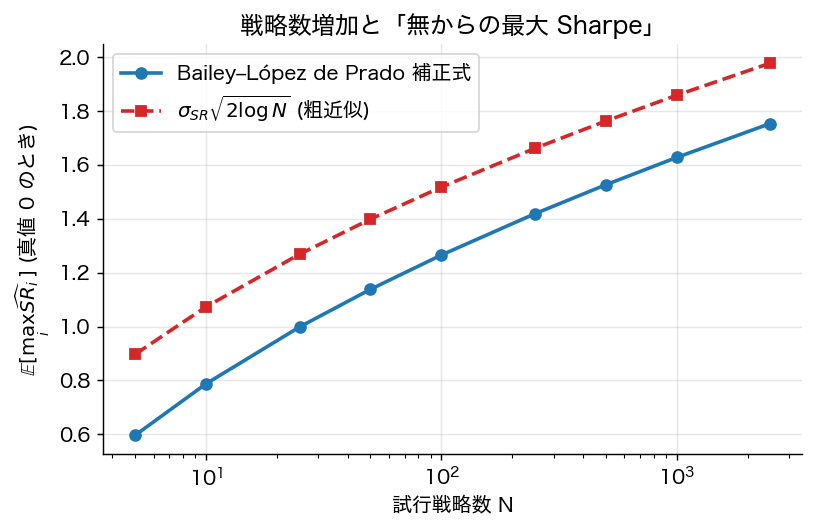
\includegraphics[width=0.85\linewidth]{figures/deflated_sharpe.png}
\caption{Sharpe 比の最大値の期待値が戦略数 $N$ にどう依存するか。$N$ が 10 から 1000 へ増えると、何もない（真の skill = 0）戦略群でも最大標本 Sharpe は 0 から 0.8〜1.5 程度まで膨らむ。}
\end{figure}

\section{16.5 機械学習バックテストの落とし穴}

\begin{itemize}
\item \textbf{ハイパーパラメタ探索}：grid search で数百〜数万通り試す。実効 $N$ は爆発。
\item \textbf{Walk-forward validation}：データ分割・リサンプリングの順序依存性。
\item \textbf{Look-ahead bias}：未来情報の漏洩。特に特性のラグ処理を間違える。
\item \textbf{Survivorship bias}：上場廃止銘柄の脱落で過大評価。
\item \textbf{データの再加工}：CRSP/Compustat の特性値が遡及的に改訂されている場合がある。
\end{itemize}

\section{16.6 健全なバックテストの設計指針}

López de Prado \emph{Advances in Financial Machine Learning} (2018) で推奨：

\begin{enumerate}
\item \textbf{Embargo + Purging}：時系列分割で IS/OOS の隣接バーを排除し情報漏洩を防ぐ。
\item \textbf{Combinatorial Purged Cross-Validation (CPCV)}：時系列での頑健な CV。
\item \textbf{試行記録}：探索したすべてのモデルを記録し $N$ を honest にカウント。
\item \textbf{DSR/PBO 計算}：報告する前に必須。
\item \textbf{Out-of-time hold-out}：絶対に触らないデータを最後の検証用に残す。
\end{enumerate}

\section{16.7 まとめ}

\begin{itemize}
\item 多戦略から最良を選ぶと標本 Sharpe は選択バイアスを受ける。
\item $\sqrt{2 \log N}$ は最大値の漸近近似だが、現実条件（相関、非正規、不明な $N$）下では粗近似。
\item DSR は標本 Sharpe を「skill 確率」に変換する診断指標。
\item PBO は「IS 優勝が OOS で凡庸化する確率」、実証的に 40–70\% と高い。
\item バックテストには purging/embargo、honest な試行カウント、out-of-time hold-out が必須。
\end{itemize}

\noindent\hrulefill

% ===== 17_derivatives_intro.md =====
\chapter{第17章 デリバティブ入門：無裁定とパリティ関係}

\begin{quote}
🎯 \textbf{この章で答える問い}
- \textbf{デリバティブ（派生証券）} とは何か。なぜ「将来の売買価格を今日決める」契約に意味があるのか。
- フォワード価格 $F_0 = S_0 e^{rT}$ はどこから来るのか — \textbf{無裁定原理} だけから出る。
- \textbf{コール・プット・パリティ} とは何で、なぜ違反したら裁定機会となるのか。

📐 \textbf{使う数学}：指数関数、現在価値割引、簡単な代数（連立方程式）。

🔑 \textbf{主要結果}：派生証券の価格は「期待値の予想」ではなく、\textbf{無裁定（一物一価）} によって決まる。
\end{quote}

これまでの章は \textbf{株式・債券などの原資産} を直接保有するポートフォリオを扱ってきた。本章からは \textbf{デリバティブ（派生証券、derivatives）} — 原資産から派生して価値を持つ契約 — を扱う。代表例：

\begin{itemize}
\item \textbf{フォワード／先物（forward/futures）}：将来時点 $T$ に資産を一定価格 $K$ で売買する契約。
\item \textbf{コール・オプション}：満期 $T$ に価格 $K$ で \textbf{買う権利}（義務ではない）を持つ契約。
\item \textbf{プット・オプション}：満期 $T$ に価格 $K$ で \textbf{売る権利}（義務ではない）を持つ契約。
\item \textbf{スワップ・CDS} などより複雑な契約は本章末の道標で名前だけ示す。
\end{itemize}

\begin{quote}
📜 \textbf{歴史 note：デリバティブは現代の発明か}

デリバティブの歴史は古く、紀元前のメソポタミアの穀物先渡契約まで遡る。17 世紀オランダのチューリップ熱もオプション取引が一因とされる。シカゴ商品取引所 (1848) で先物取引が制度化され、シカゴ・オプション取引所 (1973) でオプション市場が現代化された。Black–Scholes–Merton (1973) の \textbf{価格付け公式} は、ちょうど同年の CBOE オープンと同時に発表され、市場の急成長を後押しした。
\end{quote}

\section{17.1 一物一価と無裁定原理}

\textbf{無裁定原理 (no-arbitrage principle)}：
\begin{quote}
リスクのないポジションでお金が増える機会はない。等価キャッシュフローを生む 2 つのポートフォリオは、現時点で \textbf{同じ価格} を持たねばならない。
\end{quote}

これだけが本章のすべての公式の出発点である。\textbf{期待値も投資家の選好も使わない}。

\begin{quote}
🎯 \textbf{直観 box：無裁定はなぜ強力か}

「もしフォワード価格 $F$ が $S_0 e^{rT}$ より高すぎれば、（i）株を借りて空売り、（ii）受け取った $S_0$ を $r$ で運用、（iii）フォワードで $F$ を払い株を買い戻し空売りを閉じる」で \textbf{無リスクの利益 $F - S_0 e^{rT}$} が出る。市場参加者がこの裁定を取り尽くせば、価格は $S_0 e^{rT}$ に収束する。需要供給ではなく、\textbf{裁定の存在} が価格を決めるという考え方は派生証券論の核心。
\end{quote}

\section{17.2 フォワード価格}

\textbf{設定}：時刻 0 で「時刻 $T$ に資産を $K$ で買う」フォワード契約に入る。配当のない資産、無リスク金利 $r$（連続複利）を仮定。

\textbf{フォワード価格} $F_0$ とは、「契約価値が 0 になる行使価格 $K$」のこと： \[ \boxed{\;F_0 = S_0 e^{rT}\;} \]

\textbf{導出（無裁定論証）}：
\begin{itemize}
\item ポートフォリオ A：フォワード買い + 額面 $K$ の割引債 → 時刻 $T$ に $S_T$
\item ポートフォリオ B：現物株 1 単位（時刻 0 で $S_0$ 払う） → 時刻 $T$ に $S_T$
\item 両者は時刻 $T$ で同じキャッシュフロー → 時刻 0 で同じ価値
\item フォワード価値 0 とすると、$K e^{-rT} = S_0$、すなわち $K = F_0 = S_0 e^{rT}$
\end{itemize}

\textbf{配当のある場合}：連続配当利回り $q$ なら $F_0 = S_0 e^{(r-q)T}$。離散配当 $D$（現在価値）なら $F_0 = (S_0 - D) e^{rT}$。

\begin{figure}[H]
\centering
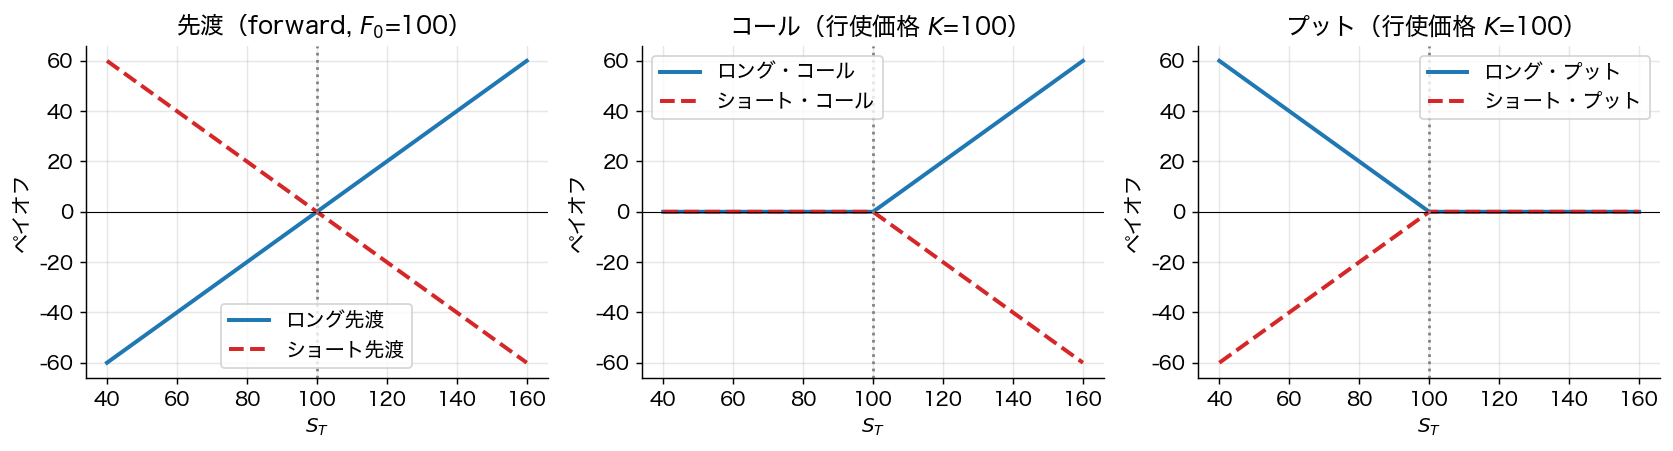
\includegraphics[width=0.85\linewidth]{figures/option_payoffs.png}
\caption{フォワード／コール／プットのペイオフ図。横軸：満期株価 $S_T$、縦軸：ペイオフ。フォワードは線形、コール・プットは「折れ線」状の非線形ペイオフ。}
\end{figure}

\section{17.3 オプションのペイオフ}

満期 $T$ におけるペイオフ：

\begin{center}
\begin{tabular}{|l|l|l|}
\hline
商品 & ロング・ペイオフ & ショート・ペイオフ \\ \hline
フォワード & $S_T - K$ & $K - S_T$ \\ \hline
コール & $(S_T - K)^+ = \max(S_T - K, 0)$ & $-\max(S_T - K, 0)$ \\ \hline
プット & $(K - S_T)^+ = \max(K - S_T, 0)$ & $-\max(K - S_T, 0)$ \\ \hline
\end{tabular}
\end{center}

「コール = 上昇に賭ける、損失限定」、「プット = 下落保険」と粗く読める。が、これは「初心者向け説明」であって完全ではない（次節）。

\begin{quote}
⚠️ \textbf{実務注意 box：「コールはレバレッジ／プットは保険」の落とし穴}

- \textbf{コールはレバレッジ}：株価が上昇しても、時間価値の減少 (theta) や IV 低下でコール価値が下がりうる。
- \textbf{プットは保険}：プレミアム（保険料）が高すぎれば期待リターンを大きく削る。満期後の下落は守れない。
- 一般に「\textbf{安価な保護}」は存在しない。市場でプットが安いときは、それを安く売ってよい理由が市場で広く認識されている時。
\end{quote}

\section{17.4 プット・コール・パリティ}

\textbf{命題 17.1}（プット・コール・パリティ） ヨーロピアン（満期にしか行使できない）コール $C$ とプット $P$（同じ $K, T$）について、配当なし資産では \[ \boxed{\; C_0 - P_0 = S_0 - K e^{-rT} \;} \]

\textbf{導出}：
\begin{itemize}
\item ポートフォリオ A：コール買い + 額面 $K$ の割引債（現在価値 $K e^{-rT}$）
\item 満期：$\max(S_T - K, 0) + K = \max(S_T, K)$
\item ポートフォリオ B：プット買い + 現物株 1 単位
\item 満期：$\max(K - S_T, 0) + S_T = \max(S_T, K)$
\item 両者のペイオフは恒等的に等しい → 現時点の価値も等しい
\item $C_0 + K e^{-rT} = P_0 + S_0$
\end{itemize}

このパリティ違反が観測されたら、瞬時に裁定機会となる。実務上、最も基本的かつ厳密に守られる制約である。

\begin{figure}[H]
\centering
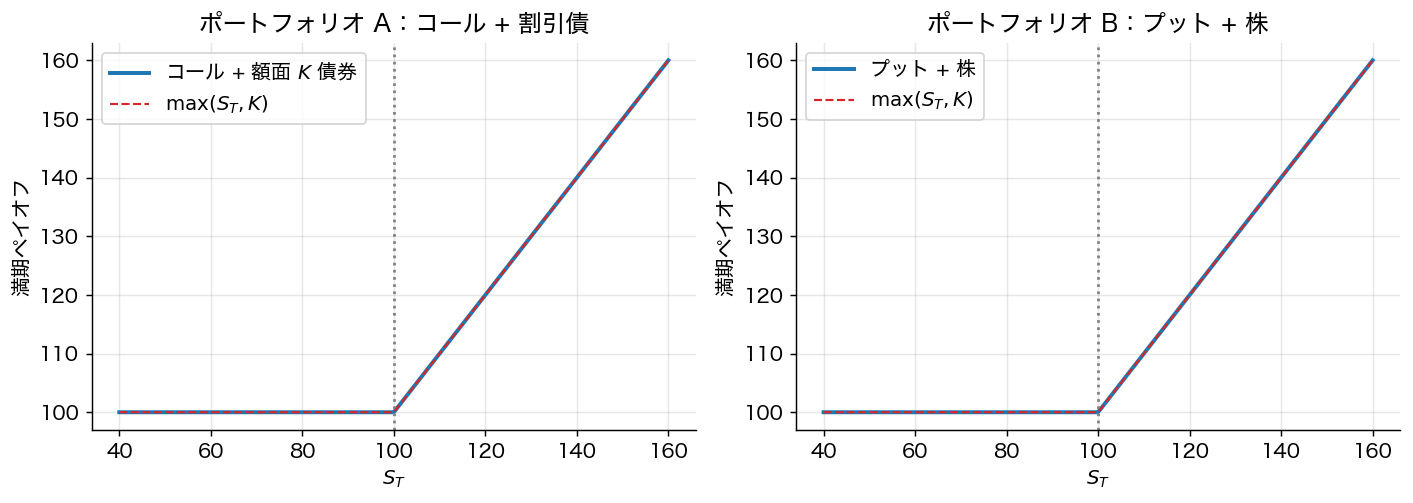
\includegraphics[width=0.85\linewidth]{figures/put_call_parity.png}
\caption{プット・コール・パリティの可視化：コール + 割引債とプット + 株のペイオフが満期で完全に重なる。}
\end{figure}

\begin{quote}
📐 \textbf{数学補足 box：複製ポートフォリオ}

パリティの導出は \textbf{「同じキャッシュフローを生む 2 つの方法は同じコスト」} という考え方だった。これは「複製ポートフォリオ」というデリバティブ評価の中心概念。第18章二項モデル、第19章 BSM でも同じ論法を繰り返し使う。
\end{quote}

\section{17.5 オプション価格の裁定範囲}

無裁定だけから、オプション価格には \textbf{必ず満たすべき不等式} が出る：

\begin{center}
\begin{tabular}{|l|l|l|}
\hline
範囲 & コール & プット \\ \hline
\textbf{下限} & $\max(S_0 - K e^{-rT}, 0) \le C_0$ & $\max(K e^{-rT} - S_0, 0) \le P_0$ \\ \hline
\textbf{上限} & $C_0 \le S_0$ & $P_0 \le K e^{-rT}$ \\ \hline
\end{tabular}
\end{center}

これらは BSM のような特定モデルを使わずに導かれる。直観：
\begin{itemize}
\item コール価格 ≤ 株価（株よりお得ではない）
\item コール価格 ≥ 「即時行使した場合の現在価値」
\end{itemize}

\begin{figure}[H]
\centering
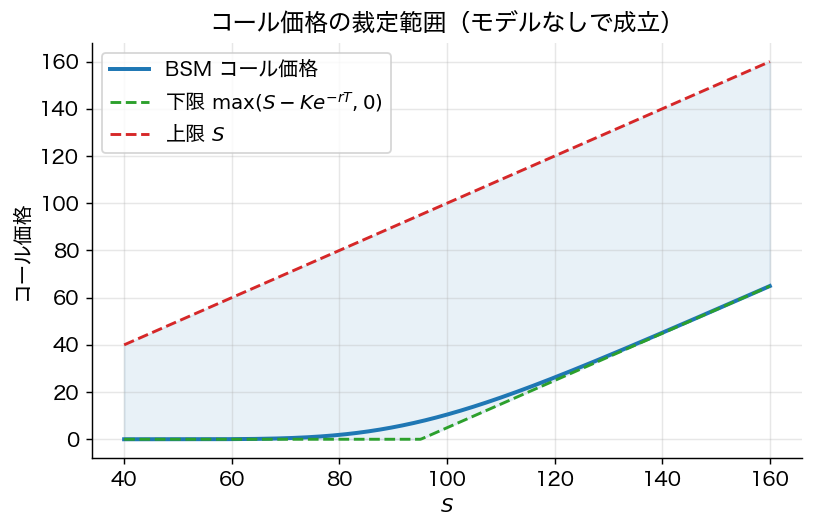
\includegraphics[width=0.85\linewidth]{figures/option_arbitrage_bounds.png}
\caption{オプション価格の裁定範囲：BSM 価格曲線とともに、満たすべき上下限を $K$ ごとに描いたもの。}
\end{figure}

\section{17.6 まとめ}

\begin{itemize}
\item デリバティブ価格は \textbf{無裁定 + 複製} だけで決まる（期待値も選好も不要）。
\item フォワード価格 $F_0 = S_0 e^{rT}$ は連続複利で割引した現在価値で表される。
\item プット・コール・パリティはオプション価格の最も基本的な制約。
\item オプション価格には BSM などのモデルなしでも裁定範囲がある。
\end{itemize}

\begin{quote}
🛣 \textbf{上級学習への道標}
- \textbf{複雑なデリバティブ}：エキゾチック・オプション（バリア、アジアン、ルックバック）、CDS、IR スワップ。Hull \emph{Options, Futures and Other Derivatives} (11th ed., 2021) が標準教科書。
- \textbf{金利モデル}：Vasicek (1977), Cox–Ingersoll–Ross (1985), Hull–White (1990)、Heath–Jarrow–Morton (1992)。
- \textbf{クレジット・デリバティブ}：強度モデル、構造モデル（Merton 1974, Black–Cox 1976）。
- \textbf{流動性・摩擦のあるデリバティブ価格}：Bid-Ask スプレッド、超複製コスト、Föllmer–Schweizer の最小リスク戦略。
\end{quote}

\noindent\hrulefill

% ===== 18_binomial_model.md =====
\chapter{第18章 二項モデルとリスク中立確率}

\begin{quote}
🎯 \textbf{この章で答える問い}
- 上下にしか動かない超単純な株価モデルで、なぜオプション価格が \textbf{一意に決まる} のか。
- \textbf{リスク中立確率} $q = (e^{r\Delta t} - d)/(u - d)$ は何を意味するのか — 実際の上昇確率ではない。
- \textbf{複製ポートフォリオ} とは何で、それがなぜ「価格そのもの」になるのか。

📐 \textbf{使う数学}：連立 1 次方程式、二項分布、現在価値の割引。

🔑 \textbf{主要結果}：1 期間二項モデルでオプション価格は \textbf{$V_0 = e^{-r\Delta t}[q V_u + (1-q) V_d]$}。これは「リスク中立確率の下での割引期待値」と読める。
\end{quote}

二項モデル (Cox–Ross–Rubinstein 1979) は、株価が「上に $u$ 倍」「下に $d$ 倍」だけ動く極端に単純なモデル。それでも \textbf{複製とリスク中立評価} の本質を全て見せる。BSM の連続時間モデルへの自然な橋渡しでもある。

\section{18.1 一期間二項モデル}

時刻 0 で株価 $S_0$、無リスク金利 $r$、時間幅 $\Delta t$。時刻 $\Delta t$ で株価は

\begin{itemize}
\item 上昇：$S_u = u S_0$（$u > 1$）
\item 下降：$S_d = d S_0$（$d < 1$）
\end{itemize}

の 2 値のみ取る。ヨーロピアン・コール（行使価格 $K$）の満期ペイオフは

\begin{itemize}
\item $V_u = (u S_0 - K)^+$
\item $V_d = (d S_0 - K)^+$
\end{itemize}

\textbf{問い}：現時点の価値 $V_0$ はいくらか？

\section{18.2 複製ポートフォリオによる価格付け}

\textbf{戦略}：株を $\Delta$ 単位、無リスク債券を額面 $B$ 単位持ったポートフォリオを作り、それが時刻 $\Delta t$ でコールと同じペイオフを生むようにする。連立式：

\[ \begin{cases} \Delta \cdot u S_0 + B e^{r \Delta t} = V_u \\ \Delta \cdot d S_0 + B e^{r \Delta t} = V_d \end{cases} \]

これを解いて

\[ \Delta = \frac{V_u - V_d}{S_0 (u - d)}, \qquad B = e^{-r\Delta t} \cdot \frac{u V_d - d V_u}{u - d}. \]

\textbf{結論}：複製ポートフォリオの現在価値が、コール価格である： \[ V_0 = \Delta \cdot S_0 + B. \]

\subsection{18.2.1 完全な手計算例（一期間コール）}

\textbf{設定}：$S_0 = 100, u = 1.2, d = 0.85, r = 0.05, \Delta t = 1$ 年、コール $K = 100$。

\textbf{Step 1}：満期ペイオフ
\begin{itemize}
\item $V_u = (1.2 \cdot 100 - 100)^+ = 20$
\item $V_d = (0.85 \cdot 100 - 100)^+ = 0$
\end{itemize}

\textbf{Step 2}：複製比率 \[ \Delta = \frac{V_u - V_d}{S_0(u - d)} = \frac{20 - 0}{100 \cdot 0.35} = 0.571. \] すなわち株 0.571 単位を保有。

\textbf{Step 3}：債券ポジション \[ B = e^{-0.05} \cdot \frac{u V_d - d V_u}{u - d} = 0.951 \cdot \frac{1.2 \cdot 0 - 0.85 \cdot 20}{0.35} = 0.951 \cdot (-48.57) = -46.20. \] すなわち額面 46.20 の債券を \textbf{発行}（借入）。

\textbf{Step 4}：コール価格 \[ V_0 = 0.571 \cdot 100 + (-46.20) = 57.10 - 46.20 = 10.90. \]

\textbf{Step 5：検証}：時刻 $\Delta t$ にこのポートフォリオがコールと同じペイオフを返すか確認：
\begin{itemize}
\item 上昇シナリオ：$0.571 \cdot 120 - 46.20 \cdot e^{0.05} = 68.52 - 48.57 = 19.95 \approx 20$ ✓
\item 下降シナリオ：$0.571 \cdot 85 - 46.20 \cdot e^{0.05} = 48.54 - 48.57 \approx 0$ ✓
\end{itemize}

完璧に複製できている。したがって \textbf{裁定なし価格は $V_0 = 10.90$}。これ以外の価格をつければ、市場参加者が複製ポートフォリオで裁定を取ることができる。

\begin{quote}
🎯 \textbf{直観 box：なぜ複製ポートフォリオの価値が「価格」になるのか}

もし $V_0$ がこれと異なれば、（i）安い方を買い、（ii）高い方を売れば、満期のペイオフが完全に相殺して \textbf{無リスクで利益} が出る。市場参加者がこの裁定を取り尽くせば、$V_0$ は複製コストに収束する。\textbf{期待値も、投資家のリスク回避度も、何の役にも立たない} — 複製コストだけが価格を決める。
\end{quote}

\section{18.3 リスク中立確率という書き直し}

上の閉じた式を整理すると、驚くべき形に書ける：

\[ \boxed{\;V_0 = e^{-r\Delta t} [q V_u + (1 - q) V_d]\;} \]

ここで \[ q = \frac{e^{r \Delta t} - d}{u - d}. \]

これは「\textbf{確率 $q$ で上昇、$1-q$ で下降する世界での }期待ペイオフ\textbf{ を、無リスク金利で割引したもの}」。$q$ を \textbf{リスク中立確率（risk-neutral probability）} と呼ぶ。

\begin{quote}
⚠️ \textbf{実務注意 box：リスク中立確率 $q$ は実際の上昇確率ではない}

学部生が最もハマる落とし穴は、$q$ を「現実に株価が上がる確率」と読むこと。これは \textbf{完全な誤解}。$q$ は「\textbf{裁定なし価格を計算するための人工的な確率}」であって、現実の確率測度 $p$ とは別物。

- $q$ の下では、株式の期待リターンは無リスク金利 $r$（リスクプレミアム 0）。これは現実とは違う。
- $p > 0.5$ でも $q < 0.5$ になりうる。
- $q$ は「割引した株価がマルチンゲール」となる \textbf{唯一の確率測度}。

「現実確率 $p$ で投資判断、リスク中立確率 $q$ で価格計算」という \textbf{2 つの確率測度の使い分け} が、本章で最も重要なポイント。
\end{quote}

\section{18.4 無裁定条件と $q$ の存在}

リスク中立確率 $q \in (0, 1)$ が存在するためには \[ d < e^{r \Delta t} < u \] が必要。これに違反すると裁定機会が生まれる：

\begin{itemize}
\item $u \le e^{r \Delta t}$：株を空売り、無リスクで運用 → 必ず勝つ。
\item $e^{r \Delta t} \le d$：株を借入で買う → 必ず勝つ。
\end{itemize}

この条件は \textbf{無裁定 ⟺ リスク中立確率の存在} という資産価格論の基本定理 (Fundamental Theorem of Asset Pricing, FTAP) の最小版である。

\section{18.5 多期間二項モデル}

満期 $T$ を $n$ ステップに分け、$\Delta t = T/n$ とする。各期で独立に上下するなら、$n$ 期後の株価分布は二項分布： \[ S_T = S_0 u^J d^{n-J}, \qquad J \sim \mathrm{Binomial}(n, q) \] （リスク中立測度の下で）。コール価格は \[ V_0 = e^{-rT} \sum_{j=0}^n \binom{n}{j} q^j (1-q)^{n-j} \cdot \max(S_0 u^j d^{n-j} - K, 0). \]

\textbf{Cox–Ross–Rubinstein のキャリブレーション}：BSM と整合する $u, d$ の設定： \[ u = e^{\sigma \sqrt{\Delta t}}, \qquad d = e^{-\sigma \sqrt{\Delta t}}, \qquad q = \frac{e^{r \Delta t} - d}{u - d}. \]

\begin{figure}[H]
\centering
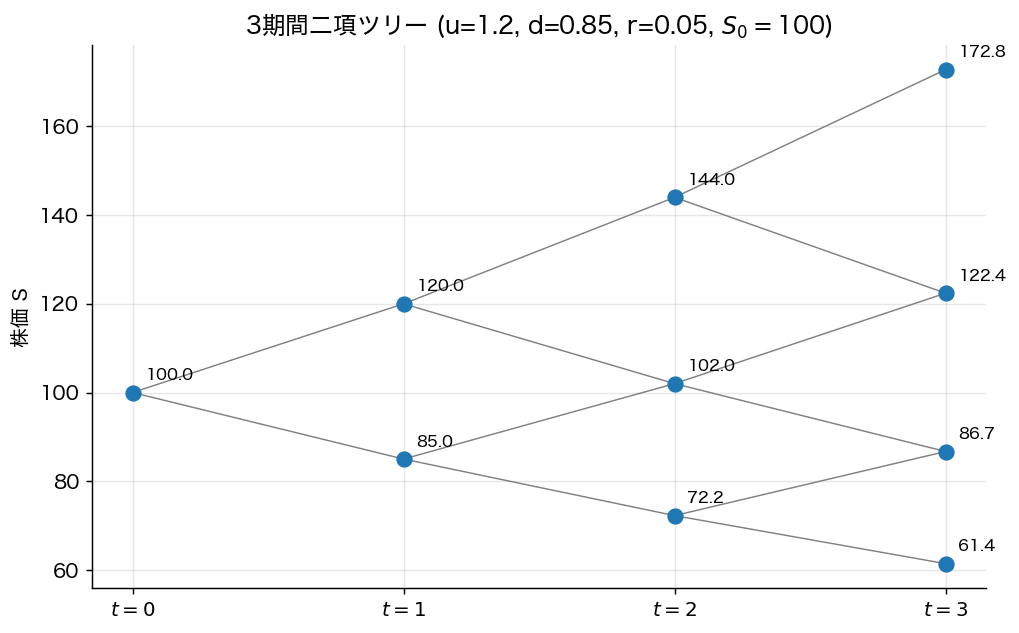
\includegraphics[width=0.85\linewidth]{figures/binomial_tree.png}
\caption{3 期間二項ツリー：各ノードに株価とオプション価値を表示。後ろ向き帰納で時刻 0 の価値を計算。}
\end{figure}

\subsection{18.5.1 3 期間ツリーの完全手計算}

$S_0 = 100, u = 1.2, d = 0.85, r = 0.05, \Delta t = 1$, $K = 100$ で、3 期間（$T = 3$）のヨーロピアン・コールを評価する。

\textbf{リスク中立確率}：$q = (e^{0.05} - 0.85)/0.35 = (1.0513 - 0.85)/0.35 = 0.575$。

\textbf{Step 1：満期 ($t=3$) の株価とペイオフ}：
\begin{itemize}
\item $S_{uuu} = 100 \cdot 1.728 = 172.8 \to V = 72.8$
\item $S_{uud} = 100 \cdot 1.224 = 122.4 \to V = 22.4$
\item $S_{udd} = 100 \cdot 0.867 = 86.7 \to V = 0$
\item $S_{ddd} = 100 \cdot 0.614 = 61.4 \to V = 0$
\end{itemize}

\textbf{Step 2：$t = 2$ への後ろ向き帰納}（割引因子 $e^{-0.05} = 0.951$）：
\begin{itemize}
\item $V_{uu} = 0.951 \cdot (0.575 \cdot 72.8 + 0.425 \cdot 22.4) = 0.951 \cdot (41.86 + 9.52) = 48.86$
\item $V_{ud} = 0.951 \cdot (0.575 \cdot 22.4 + 0.425 \cdot 0) = 0.951 \cdot 12.88 = 12.25$
\item $V_{dd} = 0.951 \cdot (0.575 \cdot 0 + 0.425 \cdot 0) = 0$
\end{itemize}

\textbf{Step 3：$t = 1$}：
\begin{itemize}
\item $V_u = 0.951 \cdot (0.575 \cdot 48.86 + 0.425 \cdot 12.25) = 0.951 \cdot (28.09 + 5.21) = 31.68$
\item $V_d = 0.951 \cdot (0.575 \cdot 12.25 + 0.425 \cdot 0) = 0.951 \cdot 7.04 = 6.70$
\end{itemize}

\textbf{Step 4：$t = 0$}： \[ V_0 = 0.951 \cdot (0.575 \cdot 31.68 + 0.425 \cdot 6.70) = 0.951 \cdot (18.22 + 2.85) = 20.04. \]

すなわち \textbf{3 期間ヨーロピアン・コールの裁定なし価格は約 $20.04$}。

\begin{figure}[H]
\centering
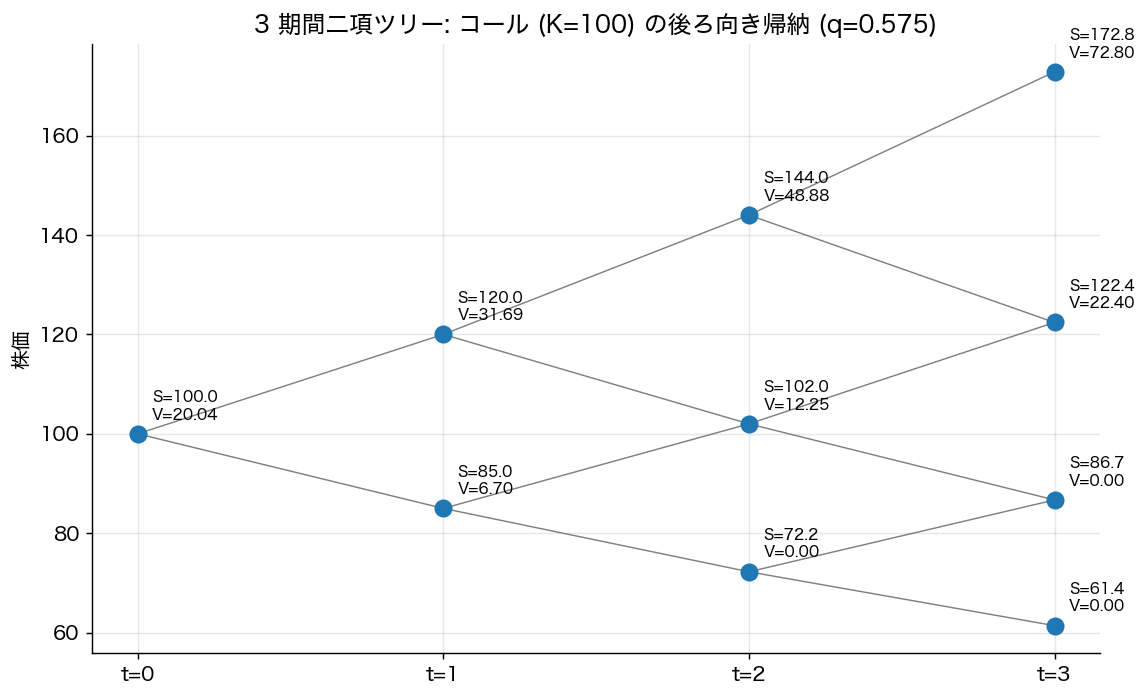
\includegraphics[width=0.85\linewidth]{figures/binomial_with_values.png}
\caption{3期間ツリー全ノードの株価と後ろ向き帰納による価値計算結果。}
\end{figure}

\begin{figure}[H]
\centering
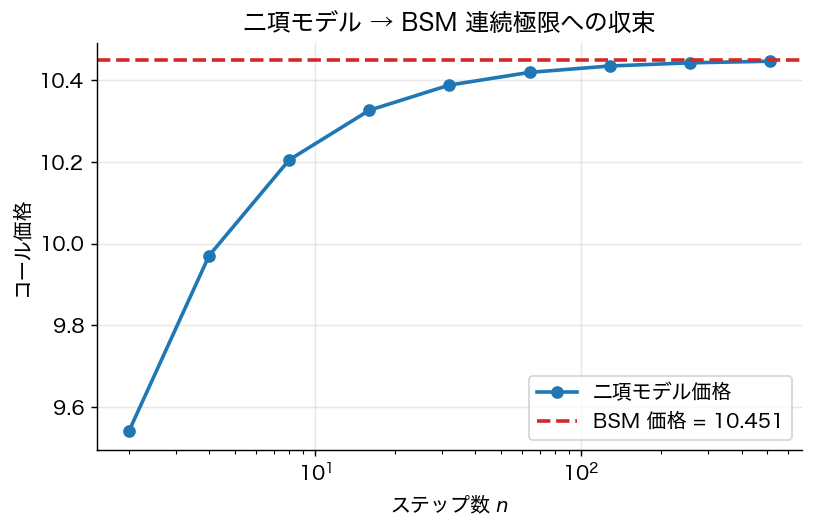
\includegraphics[width=0.85\linewidth]{figures/binomial_convergence.png}
\caption{ステップ数 $n$ を増やしたときの二項モデル価格の BSM 価格への収束（$n = 4, 16, 64, 256$）。}
\end{figure}

\section{18.6 アメリカン・オプションの扱い}

二項モデルの実務的価値は、\textbf{満期前にいつでも行使できるアメリカン・オプション} を扱えること（BSM 公式では難しい）。各ノードで \[ V_{\rm node} = \max\bigl(\,\text{即時行使ペイオフ},\ e^{-r\Delta t}[q V_u + (1-q) V_d]\,\bigr) \] として後ろ向き帰納で解く。

\begin{quote}
📐 \textbf{数学補足 box：後ろ向き帰納（Backward Induction）}

動的計画法 (Bellman) の特殊形。「最後の状態から始めて、各時点でその時点での最適決定を計算しながら時間を遡る」方法。第10章 Merton 問題の HJB 方程式も同じ原理の連続時間版。
\end{quote}

\section{18.7 BSM への極限（連続時間化のスケッチ）}

ステップ数 $n \to \infty$、$\Delta t = T/n \to 0$ の極限で何が起こるかを見る。

\begin{enumerate}
\item CRR キャリブレーションで $u = e^{\sigma \sqrt{\Delta t}}, d = e^{-\sigma \sqrt{\Delta t}}$
\item $n$ 期後の対数株価：$\log S_T = \log S_0 + (2J - n)\sigma\sqrt{\Delta t}$
\item $J \sim \mathrm{Binomial}(n, q)$ より、中心極限定理で正規分布へ収束
\item $q$ を $\Delta t$ で展開し、平均・分散を計算すると：
\end{enumerate}
\[ \log S_T \sim \mathcal{N}\!\left(\log S_0 + (r - \tfrac{1}{2} \sigma^2) T,\ \sigma^2 T\right) \] （リスク中立測度の下で）
\begin{enumerate}
\item これは \textbf{幾何ブラウン運動} $dS = r S\, dt + \sigma S\, dW$ の解と同じ分布
\end{enumerate}

すなわち二項モデルの連続極限が \textbf{BSM のリスク中立 GBM} に一致する。BSM コール価格は \[ C_0 = e^{-rT} \mathbb{E}^Q\!\bigl[(S_T - K)^+\bigr] \] の積分計算から導かれる（第19章）。

\section{18.8 まとめ}

\begin{itemize}
\item 二項モデルは「複製とリスク中立評価」の最小モデル。
\item $V_0 = e^{-r\Delta t}[q V_u + (1-q) V_d]$ は \textbf{裁定なし価格} の表現。
\item リスク中立確率 $q$ は計算用の人工確率であって現実の上昇確率ではない。
\item 多期間化と CRR キャリブレーションで BSM 連続時間モデルへ収束。
\item アメリカン・オプションを扱える点で実務的に重要。
\end{itemize}

\begin{quote}
🛣 \textbf{上級学習への道標}
- \textbf{資産価格論の基本定理 (Fundamental Theorem of Asset Pricing)}：無裁定 ⟺ 等価マルチンゲール測度の存在。Harrison–Pliska (1981), Delbaen–Schachermayer (1994) が標準的厳密版。
- \textbf{不完備市場での価格付け}：完全に複製できないオプション（ジャンプ・確率ボラ・取引費用）には複数のリスク中立測度が存在。\textbf{最小エントロピー測度} (Frittelli 2000)、\textbf{変動最小ヘッジ} (Föllmer–Schweizer 1991) などの選択基準が研究されている。
- \textbf{モンテカルロ法による多期間価格付け}：Longstaff–Schwartz (2001) の最小二乗法でアメリカン・オプションを評価。
\end{quote}

\noindent\hrulefill

% ===== 19_black_scholes.md =====
\chapter{第19章 Black–Scholes–Merton と Greeks}

\begin{quote}
🎯 \textbf{この章で答える問い}
- \textbf{Black–Scholes–Merton (BSM) 公式} $C = S_0 N(d_1) - K e^{-rT} N(d_2)$ は何を意味するのか。
- \textbf{Greeks}（$\Delta, \Gamma, \mathrm{Vega}, \Theta, \rho$）とは何で、なぜ実務で重要か。
- \textbf{インプライド・ボラティリティ (IV)} とは何で、なぜ「スマイル」になるのか。
- 連続デルタヘッジは本当に「無リスク」か？ — 離散リバランスのシミュレーションで検証する。

📐 \textbf{使う数学}：正規分布の累積分布関数 $N(\cdot)$、対数正規分布、簡単な偏微分。

⚠️ \textbf{本章の方針}：BSM の \textbf{厳密な PDE 導出}（Itô の補題 + 無裁定）は第18章の二項モデル連続極限で代用する。本章では \textbf{公式の使い方と直観} を重視。
\end{quote}

\section{19.1 BSM 公式}

\textbf{設定}：原資産の価格が幾何ブラウン運動 $dS = \mu S\, dt + \sigma S\, dW$（実確率）に従う。無リスク金利 $r$、ボラティリティ $\sigma$ 一定、配当なし、連続取引、無摩擦。

\textbf{定理 19.1}（Black–Scholes–Merton 1973） ヨーロピアン・コール（行使価格 $K$、満期 $T$）の現在価格は \[ \boxed{\; C_0 = S_0 N(d_1) - K e^{-rT} N(d_2) \;} \] ここで \[ d_1 = \frac{\log(S_0 / K) + (r + \sigma^2 / 2) T}{\sigma \sqrt{T}}, \qquad d_2 = d_1 - \sigma \sqrt{T}, \] $N(\cdot)$ は標準正規分布の累積分布関数。

プットは \textbf{パリティ} から \[ P_0 = K e^{-rT} N(-d_2) - S_0 N(-d_1). \]

\textbf{導出スケッチ}（第18章 §18.7 から）：
\begin{itemize}
\item 二項モデルの連続極限でリスク中立 GBM $dS = r S\, dt + \sigma S\, dW$
\item リスク中立期待値 $C_0 = e^{-rT} \mathbb{E}^Q[(S_T - K)^+]$
\item $\log S_T$ が正規分布 $\mathcal{N}(\log S_0 + (r - \sigma^2/2)T, \sigma^2 T)$ なので、対数正規分布の上での積分を計算
\item 結果が上式
\end{itemize}

\subsection{19.1.1 BSM 公式の段階的導出（対数正規積分）}

リスク中立期待値の積分を直接展開して BSM 公式を導く。

\textbf{Step 1}：$\log S_T \sim \mathcal{N}(m, v^2)$、$m = \log S_0 + (r - \sigma^2/2)T$、$v = \sigma\sqrt{T}$。

\textbf{Step 2}：$Z = (\log S_T - m)/v \sim \mathcal{N}(0, 1)$ に変数変換すると \[ C_0 = e^{-rT} \int_{-\infty}^\infty (e^{m + v z} - K)^+ \phi(z)\, dz. \]

\textbf{Step 3}：$S_T \ge K$ となるのは $e^{m + v z} \ge K$、すなわち $z \ge (\log K - m)/v = -d_2$（$d_2 := (m - \log K)/v$）。

\textbf{Step 4}：積分を 2 つに分割： \[ C_0 = e^{-rT}\Bigl[\,\underbrace{\int_{-d_2}^\infty e^{m + v z} \phi(z)\, dz}_{I_1} - K\, \underbrace{\int_{-d_2}^\infty \phi(z)\, dz}_{I_2}\,\Bigr]. \]

\textbf{Step 5}：$I_2$ は単純： \[ I_2 = 1 - \Phi(-d_2) = \Phi(d_2) = N(d_2). \]

\textbf{Step 6}：$I_1$ は指数項を整理。$e^{vz} \phi(z) = e^{v^2/2} \phi(z - v)$（指数の中で平方完成）より \[ I_1 = e^{m + v^2/2} \int_{-d_2}^\infty \phi(z - v)\, dz = e^{m + v^2/2} \cdot \Phi(d_2 + v). \]

\textbf{Step 7}：$m + v^2/2 = \log S_0 + r T$（$-\sigma^2 T/2 + \sigma^2 T/2 = 0$ がキャンセル）。$d_1 := d_2 + v = d_2 + \sigma\sqrt T$。

\textbf{Step 8}：代入： \[ C_0 = e^{-rT}\bigl[\,S_0 e^{rT} N(d_1) - K N(d_2)\,\bigr] = S_0 N(d_1) - K e^{-rT} N(d_2). \quad \square \]

これが \textbf{BSM 公式の積分的導出}。本質は「対数正規分布の上での片側期待値計算」。

\begin{figure}[H]
\centering
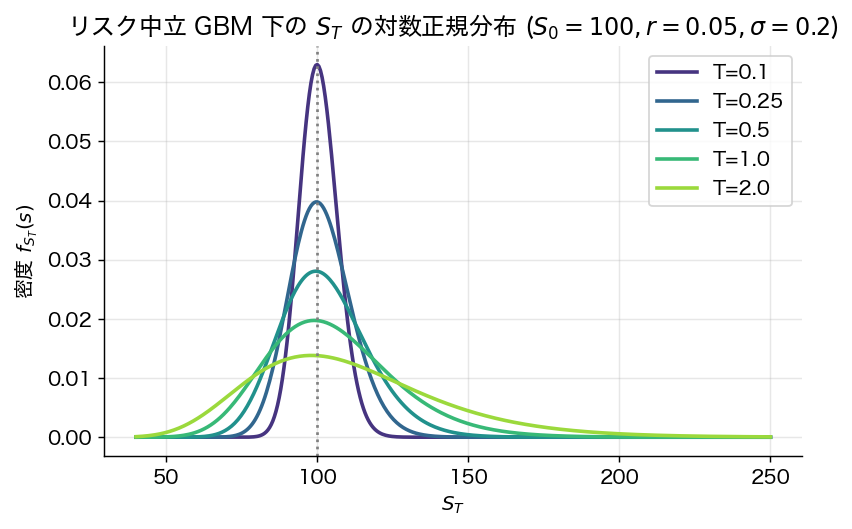
\includegraphics[width=0.85\linewidth]{figures/lognormal_evolution.png}
\caption{リスク中立 GBM 下の $S_T$ の対数正規分布。$T$ が伸びると分布が広がる。BSM 価格はこの分布の上で $\max(S_T - K, 0)$ を期待値で取ったもの。}
\end{figure}

\subsection{19.1.2 BSM 価格の手計算例}

\textbf{設定}：$S_0 = 100, K = 100, r = 0.05, T = 1, \sigma = 0.2$。

\textbf{Step 1}：$d_1, d_2$ を計算。 \[ d_1 = \frac{\log(100/100) + (0.05 + 0.02)\cdot 1}{0.2 \cdot 1} = \frac{0 + 0.07}{0.2} = 0.35. \] \[ d_2 = d_1 - 0.2 = 0.15. \]

\textbf{Step 2}：$N(d_1), N(d_2)$（標準正規分布表 or scipy.stats.norm.cdf）：
\begin{itemize}
\item $N(0.35) \approx 0.637$
\item $N(0.15) \approx 0.560$
\end{itemize}

\textbf{Step 3}：BSM コール価格： \[ C_0 = 100 \cdot 0.637 - 100 \cdot e^{-0.05} \cdot 0.560 = 63.7 - 100 \cdot 0.951 \cdot 0.560 = 63.7 - 53.3 = 10.4. \]

\textbf{Step 4}：プット価格（パリティ $C - P = S - K e^{-rT}$ から）： \[ P_0 = C_0 - S_0 + K e^{-rT} = 10.4 - 100 + 95.1 = 5.5. \]

または直接公式：$P_0 = K e^{-rT} N(-d_2) - S_0 N(-d_1) = 95.1 \cdot 0.440 - 100 \cdot 0.363 \approx 41.8 - 36.3 \approx 5.5$。一致。

\textbf{Greeks も計算}：
\begin{itemize}
\item $\Delta_C = N(d_1) = 0.637$ → 株価 1 円上昇でコール 0.64 円上昇
\item $\phi(0.35) \approx 0.375$
\item $\Gamma = 0.375/(100 \cdot 0.2 \cdot 1) = 0.0188$
\item $\mathrm{Vega} = 100 \cdot 0.375 \cdot 1 = 37.5$（per 1.00 sigma）→ 1 vol point あたり 0.375
\item $\Theta = -100 \cdot 0.375 \cdot 0.2/(2) - 0.05 \cdot 95.1 \cdot 0.560 = -3.75 - 2.66 = -6.41$（年率） → 1 日あたり約 $-0.018$
\end{itemize}

\begin{quote}
📐 \textbf{数学補足 box：$N(d_1)$ と $N(d_2)$ の意味}

- $N(d_2)$：「リスク中立確率の下で \textbf{コールが行使される確率}」$Q(S_T > K)$
- $N(d_1)$：「リスク中立確率の下で、行使条件下の \textbf{株価の現在価値による加重確率}」
- したがって BSM 公式は「\textbf{行使時の株を受け取る} $-$ \textbf{行使価格を払う}」の期待値割引版という構造を持つ

⚠️ \textbf{よくある誤解}：$N(d_2)$ は \textbf{リスク中立確率}。現実確率で行使される確率とは違う。
\end{quote}

\begin{quote}
🎯 \textbf{直観 box：BSM 価格は「期待値の予想」ではない}

BSM 価格 $C_0$ は「将来の株価を予想して期待値を取った価格」ではない。\textbf{「連続的にデルタヘッジするなら、満期ペイオフを複製するのにいくらかかるか」} という \textbf{複製コスト} を表す式である。これが入門で最もハマる点：\textbf{実確率の $\mu$（株式の真の期待リターン）は BSM 公式に登場しない}。代わりに無リスク金利 $r$ だけが出る。
\end{quote}

\begin{figure}[H]
\centering
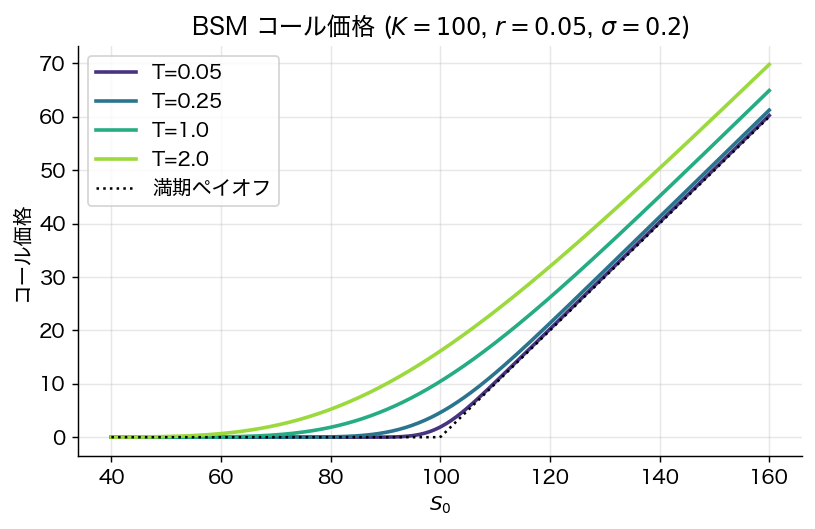
\includegraphics[width=0.85\linewidth]{figures/bsm_price_curve.png}
\caption{BSM コール価格を $S_0$ について描いたもの（満期 $T$ ごと）。満期で折れ線（ペイオフ）、満期前は滑らかな曲線。時間が経つほど ATM 周辺で価値が減る (theta decay)。}
\end{figure}

\section{19.2 Greeks（リスク感応度）}

BSM 価格を諸パラメタで偏微分したものが \textbf{Greeks}。実務でオプション・ポートフォリオのリスクを管理する核心ツール。

\subsection{19.2.1 Delta $\Delta$}
\[ \Delta_C = \frac{\partial C}{\partial S} = N(d_1), \qquad \Delta_P = N(d_1) - 1. \]

\textbf{意味}：株価が 1 円上がったときのオプション価格の上昇額。\textbf{ヘッジ比率} として最も基本。コール $\Delta \in [0, 1]$、プット $\Delta \in [-1, 0]$。

\textbf{ATM（at-the-money, $S \approx K$）} で $\Delta \approx 0.5$、\textbf{ITM（in-the-money）} で $1$ に近づき、\textbf{OTM（out-of-the-money）} で $0$ に近づく。

\subsection{19.2.2 Gamma $\Gamma$}
\[ \Gamma = \frac{\partial^2 C}{\partial S^2} = \frac{\phi(d_1)}{S_0 \sigma \sqrt{T}} \] （$\phi$ は標準正規 PDF）。\textbf{Delta が株価でどう変わるか}（曲率）。ATM・短満期で最大。

\subsection{19.2.3 Vega $\nu$}
\[ \nu = \frac{\partial C}{\partial \sigma} = S_0 \phi(d_1) \sqrt{T}. \] \textbf{ボラティリティ感応度}。ATM・長満期で最大。

\subsection{19.2.4 Theta $\Theta$}
\[ \Theta_C = -\frac{S_0 \phi(d_1) \sigma}{2 \sqrt{T}} - r K e^{-rT} N(d_2). \] \textbf{時間経過によるオプション価値の減少率}（通常負）。

\subsection{19.2.5 Rho $\rho$}
\[ \rho_C = K T e^{-rT} N(d_2). \] \textbf{金利感応度}。長満期コールほど大きい。

\begin{figure}[H]
\centering
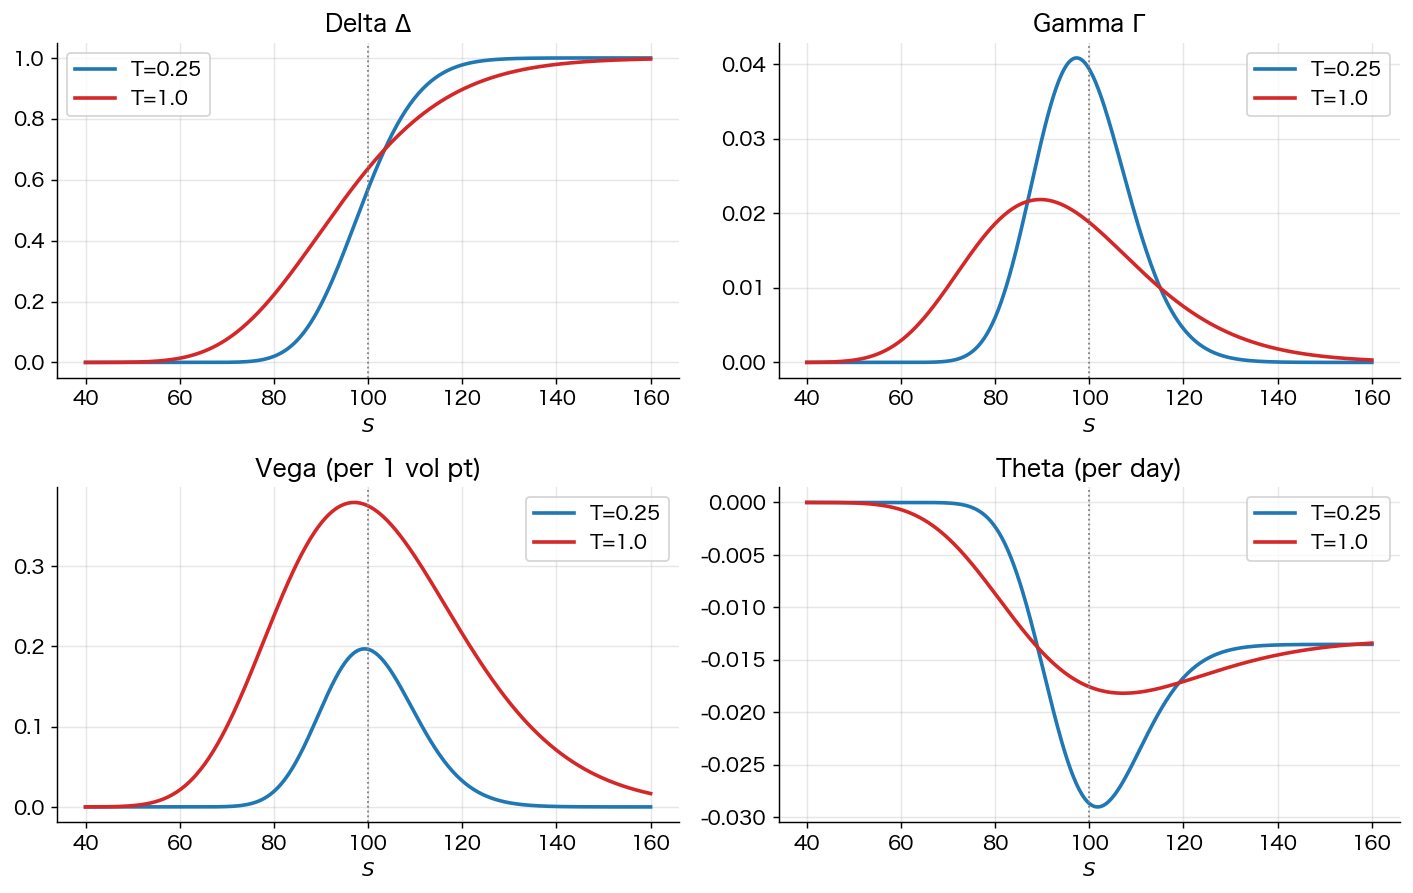
\includegraphics[width=0.85\linewidth]{figures/bsm_greeks.png}
\caption{Greeks の挙動：横軸 $S$、縦軸に Delta、Gamma、Vega、Theta を別パネルで。$K=100$ を仮定、$T = 0.25, 1$ で比較。}
\end{figure}

\begin{quote}
⚠️ \textbf{実務注意 box：Greeks の代表的な誤解}

1. \textbf{$\Delta$ を「行使される確率」と読む}：$\Delta = N(d_1)$ は厳密には行使確率（$N(d_2)$）と違う。
2. \textbf{$\Gamma$ を無視して $\Delta$ が一定だと思う}：株価が大きく動くと $\Delta$ も動く（曲率効果）。
3. \textbf{$\Theta$ は売り手に有利と単純化}：時間価値減少は売り手の儲けだが、その間ボラが上がると損する。
4. \textbf{Vega は満期直前に最大と思う}：実は \textbf{ATM・長満期} で最大。
5. \textbf{Vega の単位}：BSM 標準では「$\sigma$ が $1.00$ 増えた時の価格変化」（$0.20 \to 1.20$）。実務では「1 vol point ($0.20 \to 0.21$)」あたりに換算するため $/ 100$ することが多い。
\end{quote}

\section{19.3 デルタヘッジと P\&L}

オプションを売った市場メイカーは、自分のポジションを \textbf{デルタ中立} にすることでリスク軽減を図る。コールを 1 単位売ったら、株を $\Delta$ 単位買って保有する： \[ \text{ポートフォリオ価値} = -C + \Delta \cdot S. \]

理論的には連続的に $\Delta$ を再調整すれば \textbf{完全ヘッジ}。実際は離散リバランスなので \textbf{ヘッジ誤差} が残る。

\begin{figure}[H]
\centering
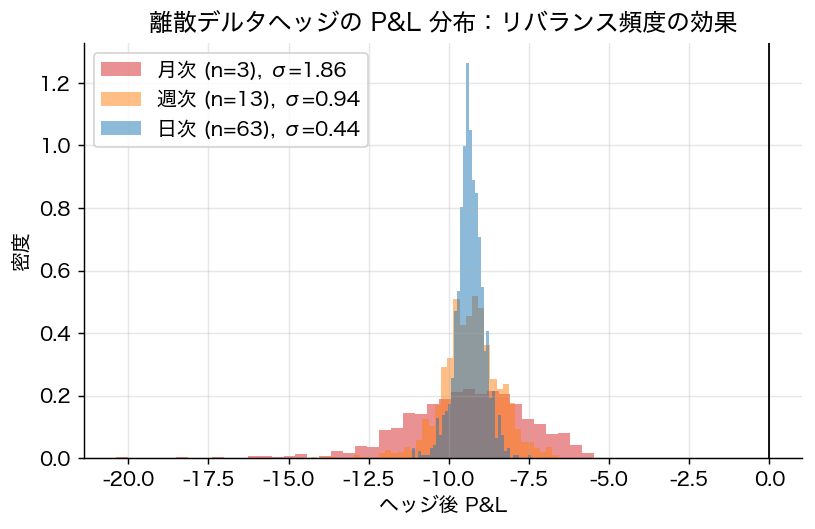
\includegraphics[width=0.85\linewidth]{figures/delta_hedge_pnl.png}
\caption{離散デルタヘッジのシミュレーション：毎日リバランス（$N=252$）と毎月リバランス（$N=12$）の P\&L 分布の比較。リバランス頻度が低いほど P\&L のばらつきが大きい。}
\end{figure}

\subsection{19.3.1 デルタヘッジ P\&L の分解：Gamma・Theta・Vega}

連続デルタヘッジ下で、オプション売り手の \textbf{微小時間 P\&L} は次のように分解できる（Itô の補題から）： \[ dP = \left[-\Theta - \tfrac{1}{2} \Gamma S^2 \sigma_{\rm impl}^2\right] dt + \tfrac{1}{2} \Gamma (dS)^2 + \nu\, d\sigma_{\rm impl} + \cdots \]

直観的に：
\begin{itemize}
\item \textbf{Theta} $\Theta < 0$：時間経過で BSM 価値が減る → 売り手の \textbf{利益}
\item \textbf{Gamma} $\Gamma > 0$：株価変動 $(dS)^2$ → 売り手の \textbf{損失}（買い手の利益）
\item \textbf{Vega} $\nu > 0$：IV 変動 → 売り手は IV 上昇で \textbf{損失}
\end{itemize}

\textbf{ボラティリティ取引の本質}：「\textbf{実現ボラ vs インプライド・ボラ}」の差で儲かる／損する：
\begin{itemize}
\item 実現ボラ > インプライド ⇒ Gamma 損失 > Theta 利益 ⇒ 売り手は損
\item 実現ボラ < インプライド ⇒ Gamma 損失 < Theta 利益 ⇒ 売り手は得
\end{itemize}

これが「\textbf{オプション売りはボラ売り戦略}」と呼ばれる所以。

\begin{figure}[H]
\centering
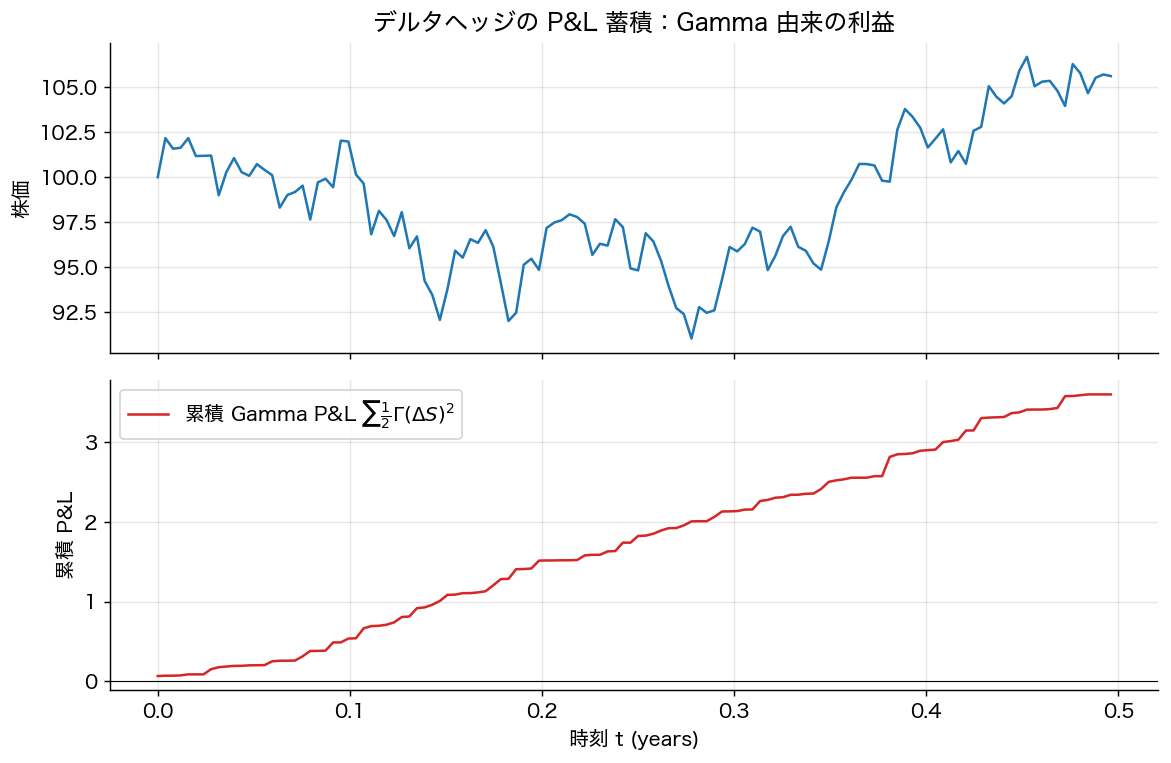
\includegraphics[width=0.85\linewidth]{figures/delta_hedge_decomp.png}
\caption{単一パスでのデルタヘッジ P\&L の累積：Gamma 由来の蓄積。株価変動が大きいほど累積 P\&L が増える。}
\end{figure}

\begin{quote}
🎯 \textbf{直観 box：「BSM 価格 = 動的複製コスト」が腑に落ちる場面}

オプションを売って $C_0$ を受け取り、デルタヘッジで株を売買し続ける。\textbf{もし $\sigma$ の予想が正しく、連続リバランスができれば、累積した株売買コストと借入金利の合計は最終的に $C_0$ にぴたり一致する}。すなわち $C_0$ は「複製コスト」そのもの。実際は離散ヘッジによる誤差が残るが、誤差の標準偏差は $\sqrt{\Delta t}$ で減る。
\end{quote}

\section{19.4 インプライド・ボラティリティ}

市場で観測されたオプション価格 $C_{\rm mkt}$ について、BSM 公式を逆向きに解いて $\sigma$ を求めたものが \textbf{インプライド・ボラティリティ (Implied Volatility; IV)}： \[ C_{\rm mkt} = C_{\rm BS}(S_0, K, r, T, \sigma_{\rm imp}). \]

$\sigma_{\rm imp}$ は「市場が考えるボラティリティ」と解釈される。

\subsection{19.4.0 Newton 法で IV を逆算する}

IV は BSM 公式を $\sigma$ について解くため、\textbf{反復的に求める}：

\textbf{Newton 法のアルゴリズム}：
\begin{enumerate}
\item 初期推定 $\sigma_0 = 0.3$ などを置く
\item $C_{\rm BS}(\sigma_k)$ を計算
\item Vega を計算：$\nu_k = S_0 \phi(d_1) \sqrt{T}$
\item 更新：$\sigma_{k+1} = \sigma_k - (C_{\rm BS}(\sigma_k) - C_{\rm market})/\nu_k$
\item $|\sigma_{k+1} - \sigma_k| < 10^{-6}$ で収束
\end{enumerate}

通常 3-5 反復で収束する（Vega が正で滑らかなので Newton は安定）。

\begin{figure}[H]
\centering
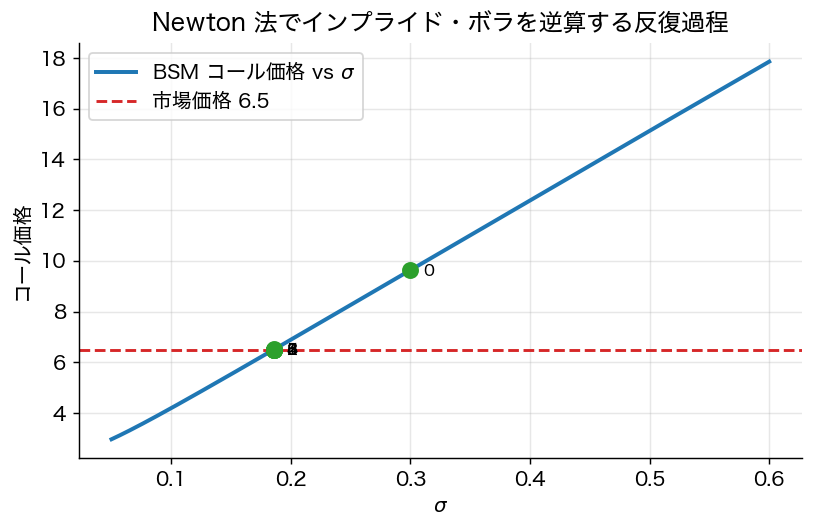
\includegraphics[width=0.85\linewidth]{figures/iv_newton.png}
\caption{Newton 法の IV 逆算過程：BSM 価格 vs σ 曲線上を反復が市場価格に収束する様子。}
\end{figure}

\subsection{IV スマイル}

BSM が現実なら、行使価格 $K$ にかかわらず IV は一定のはず。しかし実際は：
\begin{itemize}
\item \textbf{株式オプション}：低 $K$（OTM プット）で IV が高い → \textbf{スキュー}（右下がり）
\item \textbf{為替・コモディティ}：両側で IV が高い → \textbf{スマイル}
\end{itemize}

理由：
\begin{enumerate}
\item \textbf{テールリスク}（クラッシュ）の警戒
\item ボラティリティ自体の不確実性（\textbf{確率ボラティリティ}）
\item 需給（プット保険の需要）
\end{enumerate}

\begin{figure}[H]
\centering
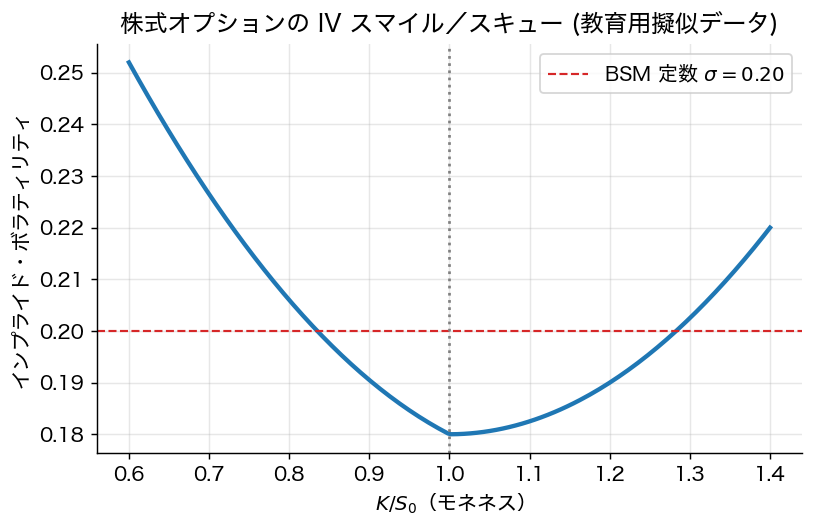
\includegraphics[width=0.85\linewidth]{figures/iv_smile.png}
\caption{株価オプションの IV スマイル（疑似データ）。横軸 $K/S_0$、縦軸 IV。OTM プット側で IV が高く、ATM で最低。}
\end{figure}

\section{19.5 BSM の前提と実務的修正}

BSM の前提と現実のズレ：

\begin{center}
\begin{tabular}{|l|l|}
\hline
前提 & 現実 \\ \hline
GBM（連続価格） & ジャンプ（決算、ニュース） \\ \hline
定数 $\sigma$ & 時変・ランダムボラ \\ \hline
連続取引 & 離散リバランス、取引費用 \\ \hline
無摩擦 & bid-ask、流動性プレミアム \\ \hline
配当なし & 配当あり（個別株、指数） \\ \hline
\end{tabular}
\end{center}

\textbf{実務的補正}：
\begin{itemize}
\item \textbf{配当}：$d_1, d_2$ で $r$ を $r - q$ に置換（連続配当利回り $q$）。
\item \textbf{確率ボラティリティ}：Heston (1993) モデル。$\sigma$ 自身が確率過程に従う。
\item \textbf{ジャンプ拡散}：Merton (1976)、Kou (2002)。クラッシュ確率を明示的にモデル化。
\end{itemize}

\begin{quote}
📐 \textbf{学部生向け段落：BSM はなぜまだ使われるのか}

BSM の前提は現実と乖離している。それでも実務で第一線で使われ続けている理由は：

1. \textbf{共通言語}：オプション価格を「インプライド・ボラ」という統一指標で議論できる。
2. \textbf{Greeks の解釈}：価格そのものよりも「$\Delta$ ヘッジ比率」「$\Gamma$ 曲率」「Vega 感応度」が重要で、これらは BSM の枠組みで計算しやすい。
3. \textbf{校正されたモデル}：BSM 価格を真実とは思わない。IV を時間・$K$ ごとに変える「市場が校正したパラメタ」として扱う。

つまり BSM は「絶対的な価格モデル」ではなく「\textbf{業界の共通座標系}」。
\end{quote}

\section{19.6 オプションとパフォーマンス評価（第11章との接続）}

オプション戦略は \textbf{歪んだリターン分布} を生むため、Sharpe 比だけで評価すると危険：

\textbf{例}：毎月 OTM プットを売る（\textbf{ボラティリティ売り} 戦略）
\begin{itemize}
\item 11 か月：毎月 $+1\%$ 利益（プレミアム回収）
\item 1 か月：暴落で $-25\%$
\item 平均月次リターン：$(11 \times 1\% - 25\%)/12 = -1.17\%$
\item だがクラッシュ前の 11 か月だけ見ると、$\sigma \approx 0$, Sharpe 比 $= \infty$ に見える
\end{itemize}

\textbf{教訓}：
\begin{itemize}
\item \textbf{Sortino 比}：下方リスクのみペナルティ。
\item \textbf{Calmar 比}：最大ドローダウン考慮。
\item \textbf{CVaR}：テール損失の平均（第8章）。
\item \textbf{シナリオ分析}：「もし 5σ 下落が来たら」の試算。
\end{itemize}

ヘッジファンドや投資銀行のオプション戦略評価ではこれらの併用が必須。

\section{19.7 まとめ}

\begin{itemize}
\item BSM 公式は「\textbf{動的複製コスト}」を与え、実確率の $\mu$ には依存しない。
\item Greeks ($\Delta, \Gamma, \mathrm{Vega}, \Theta, \rho$) はリスク管理の核心ツール。
\item インプライド・ボラティリティは市場の共通言語、スマイル／スキューが BSM 前提のズレを示す。
\item BSM の前提は現実で破られるが、\textbf{校正された IV と Greeks} で実務的に補正される。
\item オプション戦略は歪んだ分布を生むため、Sharpe 比単独では評価不能。
\end{itemize}

\begin{quote}
🛣 \textbf{上級学習への道標}
- \textbf{確率ボラティリティ・ジャンプ拡散モデル}：Heston (1993), SABR (Hagan et al. 2002), Bates (1996), Kou (2002)、Merton (1976)。
- \textbf{局所ボラティリティ}：Dupire (1994), Derman–Kani (1994)。
- \textbf{ボラティリティ・サーフェスの校正}：実務的には数値最適化問題。Gatheral \emph{The Volatility Surface} (2006) が標準書。
- \textbf{ラフ・ボラティリティ}：Gatheral–Jaisson–Rosenbaum (2018, \emph{Quantitative Finance} 18) — ボラがブラウン運動より「ラフ」な経路を持つことの実証と理論。
- \textbf{ニューラルネット・オプション価格}：Hutchinson–Lo–Poggio (1994) から始まり、近年は Deep Hedging (Buehler et al. 2019)、ニューラル PDE 解法など。
\end{quote}

\noindent\hrulefill

% ===== 20_exercises.md =====
\chapter{第17章 演習問題}

\begin{quote}
🎯 \textbf{演習の進め方}

本書の演習は 3 カテゴリ・3 難度で構成する。

| 記号 | カテゴリ | 想定時間 | 必修／選択 |
|---|---|---|---|
| ★ | \textbf{計算問題}（手で解ける） | 15–30 分 | \textbf{必修} |
| ★★ | \textbf{シミュレーション問題}（Python 推奨） | 1–3 時間 | 選択（プログラミング既習者） |
| ★★★ | \textbf{考察問題}（言葉で答える） | 30–60 分 | 卒研準備 |

本書を読むうえで \textbf{★ 問題は必修}、★★ は Python 環境がある読者の発展課題、★★★ は卒研で扱うテーマ選定の練習である。

📝 \textbf{★★★ 考察問題の評価軸}（各問の末尾に「採点のポイント」を記載）：
- 主張に対する \textbf{賛否の論理} が一貫しているか
- 教科書の \textbf{どの理論を引用したか} が明示されているか
- \textbf{限界（caveat）} にも触れているか
- 数値例・反例で補強できているか
\end{quote}

\begin{quote}
⚠️ \textbf{Python 環境について}

★★ 問題を解く場合、本書のリポジトリ直下の \texttt{.venv} を使うか、\texttt{pip install numpy scipy matplotlib scikit-learn} した環境で実行できる。データは Kenneth French のサイト、Yahoo Finance API、CRSP/Compustat（大学のサブスクリプション）等から取得する。
\end{quote}

\section{第1–2章：Markowitz と効率的フロンティア}

\textbf{問題 1.0（★／計算問題）} 2 つのリスク資産 A, B について $\mu_A = 0.08$, $\mu_B = 0.04$, $\sigma_A = 0.20$, $\sigma_B = 0.10$, $\rho_{AB} = 0.2$ とする。資産 A への投資比率を $w$、資産 B への投資比率を $1 - w$ とする。

\begin{enumerate}
\item ポートフォリオの期待リターンを $w$ の関数として書け。
\item ポートフォリオ分散を $w$ の関数として書け。
\item 分散を最小にする $w$ を求めよ。
\item そのときの期待リターンと標準偏差を計算せよ。
\end{enumerate}

\textbf{問題 1.1（★）} 2 資産（$\mu = (0.08, 0.12)^\top$、$\sigma_1 = 0.15$、$\sigma_2 = 0.25$、相関 $\rho = 0.3$）について、GMV ポートフォリオの重みと分散を求めよ。

\textbf{問題 1.2（★★）} $\Sigma = \sigma^2 I_n$（独立同分散）のとき、効率的フロンティアを陽に表せ。$n \to \infty$ で何が起こるか考察せよ。

\textbf{問題 1.3（★★★）} ショート禁止制約 $w \ge 0$ の下で、効率フロンティアが \textbf{区分的双曲線} であることを active set 分析で示せ。

\textbf{問題 2.1（★）} 3 資産で $r_f = 0.02$、$\mu = (0.06, 0.10, 0.14)^\top$、$\Sigma = \mathrm{diag}(0.01, 0.04, 0.09) + 0.005\, \mathbf{1}\mathbf{1}^\top$ とする。接線ポートフォリオを計算し、最大シャープ比を求めよ。

\textbf{問題 2.2（★★）} ゼロ β 同伴ポートフォリオの期待リターン公式（命題 2.2）を導出せよ。

\section{第3–4章：分離定理と CAPM}

\textbf{問題 3.1（★）} リスク回避度 $\gamma$ の二次効用について、無リスク資産と接線ポートフォリオへの配分比を求めよ。

\textbf{問題 4.1（★★）} $n$ 資産のリターンを観測した。サンプル共分散行列の固有値構造から市場ポートフォリオを推定する手順を Fama–MacBeth 二段階回帰の枠組みで述べよ。

\textbf{問題 4.2（★★★）} Roll 批判の数学的内容を述べ、観測されたプロキシポートフォリオが効率的でない場合に、CAPM 検定の null 仮説が成立しないことを示せ。

\begin{quote}
📝 \textbf{採点のポイント}
- 「真の市場ポートフォリオ」が観測不能であることの議論があるか
- プロキシ（株価指数）の効率性と CAPM の検証可能性の関係に言及しているか
- Fama–MacBeth 検定が「実は別の仮説のテスト」になることに気づいたか
- 反例として何を挙げられるか（不動産・人的資本・海外資産の除外、等）
\end{quote}

\section{第5章：APT}

\textbf{問題 5.1（★★）} 2 ファクターモデル $R_i = \mu_i + b_{i1} f_1 + b_{i2} f_2 + \varepsilon_i$ で $n \to \infty$ における裁定ポートフォリオを陽に構築し、定理 5.1 の証明を補強せよ。

\textbf{問題 5.2（★★）} Fama–French 3 因子モデルの月次データ（Kenneth French のウェブサイトから取得可能）を用いて、ある産業ポートフォリオの α を推定する Python コードを書け。

\section{第6–7章：効用理論と確率支配}

\textbf{問題 6.1（★）} CRRA 効用 $u(c) = c^{1-\gamma}/(1-\gamma)$ について ARA, RRA を計算し、$\gamma \to 1$ で対数効用になることを示せ。

\textbf{問題 6.2（★★）} リターンが対数正規分布 $\log(1 + R) \sim \mathcal{N}(m, s^2)$ のとき、CRRA 効用最大化問題を解いて最適投資比率を求めよ。

\textbf{問題 7.1（★★）} $X \sim \mathrm{Uniform}(0,1)$、$Y \sim \mathrm{Beta}(2, 2)$ について FSD/SSD 関係を判定せよ。

\textbf{問題 7.2（★★★）} 平均分散効率なポートフォリオが SSD 効率でない反例を構築せよ。

\section{第8章：リスク尺度}

\textbf{問題 8.1（★）} $L \sim \mathcal{N}(\mu, \sigma^2)$ について $\mathrm{VaR}_\alpha$ と $\mathrm{CVaR}_\alpha$ を陽に求めよ。

\textbf{問題 8.2（★★）} 8.3 節の反例（独立デフォルト債）を一般化し、VaR が劣加法性を破るパラメタ範囲を特定せよ。

\textbf{問題 8.3（★★★）} Rockafellar–Uryasev の補助関数 $F_\alpha(w, \zeta)$ が $\zeta$ について凸であり、最小値が CVaR に等しいことを証明せよ。

\section{第9章：Black–Litterman}

\textbf{問題 9.1（★★）} 3 資産で view が「資産 1 と 2 の平均は資産 3 より 3\% 高い」とするとき、$P, Q$ を書き下し、$\Omega$ を He–Litterman 法で設定する手順を示せ。

\textbf{問題 9.2（★★★）} 事後分布の式 9.4 を完全平方の整理から導出せよ。

\section{第10章：連続時間最適化}

\textbf{問題 10.1（★★）} CRRA 効用の Merton 問題で値関数 $V(t, x) = h(t) x^{1-\gamma}/(1-\gamma)$ と推測し、$h(t)$ の ODE を導け。

\textbf{問題 10.2（★★★）} 2 危険資産・確率ボラティリティ（Heston モデル）の最適投資問題で、ヘッジ需要項を陽に書き下せ。

\textbf{問題 10.3（★★★）} Cox–Huang のマーチンゲール法を用いて、CRRA 投資家の終末富と消費を陽に求めよ。

\section{第11章：パフォーマンス評価}

\textbf{問題 11.1（★）} 年率 Sharpe 比 0.8 のファンドを、5\% 有意水準で「skill > 0」と検出するに必要な最低期間（年）を概算せよ。

\textbf{問題 11.2（★★）} 独立に 1000 通りの戦略をバックテストし、最大の標本 Sharpe を選んだ。真の Sharpe がすべてゼロのとき、その期待値の概算式を示せ。

\textbf{問題 11.3（★★）} Sortino 比、Calmar 比、Sharpe 比のいずれが「ヘッジファンドのパフォーマンス比較」に最適か議論せよ。

\section{総合演習}

\textbf{問題 T.1（★★★）} S\&P 500 構成銘柄の日次リターン（過去 10 年）から共分散行列を推定し、(a) 標本共分散、(b) Ledoit–Wolf 縮約、(c) Fama–French 3 因子モデルベースで、それぞれ接線ポートフォリオを構築せよ。アウト・オブ・サンプル Sharpe を比較せよ。

\textbf{問題 T.2（★★★）} Black–Litterman ベイズフレームワークを用いて、グローバル株式・債券・コモディティの戦略的アセットアロケーションを設計せよ。市場ポートフォリオ・自身の view・$\Omega$ の選択を明示し、ポートフォリオの感度解析を行え。

\textbf{問題 T.3（★★★）} Merton 問題に税金（短期/長期キャピタルゲイン税の違い）を導入したときの最適政策を考察せよ。理論的考察と数値シミュレーションの両方を行え。

\section{第12章：縮小推定}

\textbf{問題 12.1（★★）} $\Sigma = I$ で $p = T = 100$ のとき、Marčenko–Pastur 分布の最大・最小固有値の理論値を計算し、シミュレーションで確認せよ。

\textbf{問題 12.2（★★★）} Ledoit–Wolf 線形縮小強度の oracle 式を Frobenius 損失のバイアス–分散分解から導出せよ。標本から推定する $\hat\alpha$ の表式も書け。

\section{第13章：ロバスト最適化}

\textbf{問題 13.1（★★）} 楕円体不確実性 $(\mu - \hat\mu)^\top \Theta^{-1} (\mu - \hat\mu) \le \kappa^2$ の下で $\min_\mu w^\top \mu = w^\top \hat\mu - \kappa \sqrt{w^\top \Theta w}$ を Cauchy–Schwarz から示せ。

\textbf{問題 13.2（★★★）} Garlappi–Uppal–Wang の閉形式縮小を、Bayesian 事前 $\mu \sim \mathcal{N}(\hat\mu, \Sigma/\tau)$ と max–min 効用から導出せよ。

\section{第14章：Risk Parity と HRP}

\textbf{問題 14.1（★）} 3 資産で $\sigma_1 = 0.10$, $\sigma_2 = 0.20$, $\sigma_3 = 0.30$, 相関すべて $0.3$ のとき、ERC ポートフォリオを数値的に求めよ。

\textbf{問題 14.2（★★）} 凸プログラム $\min_y \tfrac{1}{2} y^\top \Sigma y - \sum \log y_i$ の最適性条件から ERC 条件を導け。一意性を示せ。

\textbf{問題 14.3（★★★／実装込み）} HRP を Python で実装し、S\&P500 銘柄サブセットで GMV（LW縮小）、ERC、HRP の OOS Sharpe を比較せよ。期間・銘柄選択への感度を議論せよ。

\begin{quote}
📝 \textbf{採点のポイント}
- 3 手法の理論的な違い（$\Sigma^{-1}$ を使うか、リスク寄与均等化か、階層クラスタか）が言えているか
- OOS Sharpe の比較で「データ依存性」「期間依存性」に正直に触れているか
- HRP の「OOS で勝つ」主張に対して Jain–Jain (2019) 等の反証文献を引用できているか
- 結論として「どんな状況でどの手法を使うべきか」の判断軸を示せたか
\end{quote}

\section{第15章：因子動物園・機械学習}

\textbf{問題 15.1（★）} $N = 316$ ファクター、$\alpha = 0.05$ のとき、Bonferroni 補正後の $t$ 閾値を求めよ。BH 法と比較せよ。

\textbf{問題 15.2（★★★）} Gu–Kelly–Xiu 風に、scikit-learn と LightGBM で月次リターン予測を実装せよ。線形回帰・ランダムフォレスト・ニューラルネットを比較し、特徴量重要度を分析せよ。

\section{第16章：バックテスト過剰適合}

\textbf{問題 16.1（★）} $N = 1000$, $\sigma_{\rm SR} = 0.5$ のとき、Bailey–López de Prado の Euler 補正式と $\sigma_{\rm SR}\sqrt{2 \log N}$ の差を計算せよ。

\textbf{問題 16.2（★★）} CSCV による PBO 推定を Python で実装し、ランダム生成された 100 戦略について PBO を計算せよ。

\section{第17章：デリバティブ入門}

\textbf{問題 17.1（★）} $S_0 = 100$, $r = 0.05$, $T = 0.5$, 配当なしのとき、フォワード価格を求めよ。次に同じ条件で連続配当利回り $q = 0.02$ ならフォワード価格はいくらか。

\textbf{問題 17.2（★）} $S_0 = 100$, $K = 100$, $r = 0.05$, $T = 1$ で市場でコール価格が $C = 12$、プット価格が $P = 5$ と観測された。プット・コール・パリティは成立しているか。違反していれば、どんな裁定戦略が組めるか説明せよ。

\textbf{問題 17.3（★★★／考察）} 「コール買いは下値リスク限定の上、無限大の上昇益が得られる夢のポジションだ」という主張に対し、初心者投資家へのアドバイスを書け。

\begin{quote}
📝 \textbf{採点のポイント}
- 時間価値の減少、IV 低下、満期、流動性スプレッドのいずれかに触れているか
- 「BSM 価格 ≠ 期待値の予想」という洞察があるか
- 1 ドル動いてもコール価格が 1 ドル動かない（$\Delta < 1$）ことを説明できているか
\end{quote}

\section{第18章：二項モデル}

\textbf{問題 18.1（★）} $S_0 = 100$, $u = 1.2$, $d = 0.85$, $r = 0.05$, $\Delta t = 1$ の 1 期間モデル。リスク中立確率 $q$ を求めよ。コール（$K = 100$）の現在価値を計算せよ。複製ポートフォリオ $(\Delta, B)$ も求めよ。

\textbf{問題 18.2（★★）} 3 期間 CRR ツリー（$\sigma = 0.25, T = 0.25$）を実装し、ヨーロピアン・コールとアメリカン・プットの価格を比較せよ。アメリカン・プットの早期行使はどこで発生するか。

\textbf{問題 18.3（★★★／考察）} 「リスク中立確率 $q$ は \textbf{市場参加者が本当はリスク中立だから出てくる確率} だ」という主張を批判せよ。

\begin{quote}
📝 \textbf{採点のポイント}
- $q$ は計算用の人工確率であり、現実確率 $p$ と異なることを明示
- 無裁定条件 $d < e^{r\Delta t} < u$ の必然性に触れているか
- 「割引株価がマルチンゲール」となる確率測度として位置づけているか
\end{quote}

\section{第19章：BSM と Greeks}

\textbf{問題 19.1（★）} $S_0 = 100, K = 100, r = 0.05, T = 1, \sigma = 0.2$ で BSM コール価格を計算せよ。同じパラメタでプット価格を計算し、プット・コール・パリティを確認せよ。

\textbf{問題 19.2（★★）} Python で BSM 価格関数と Greeks（$\Delta, \Gamma, \mathrm{Vega}, \Theta$）を実装せよ。$S$ を 50〜150 でグラフ化し、$T = 0.1, 1$ で挙動の違いを観察せよ。

\textbf{問題 19.3（★★／実装込み）} 離散デルタヘッジを Monte Carlo シミュレーション（1000 経路）で実装。リバランス頻度（日次／週次／月次）による P\&L 分布のばらつきを比較せよ。

\textbf{問題 19.4（★★★／考察）} 「Sharpe 比 = 3.0」を売り文句とする systematic option selling 戦略のファンドがあった。投資判断として、追加でどんなデータ・分析を求めるか挙げよ。

\begin{quote}
📝 \textbf{採点のポイント}
- リターン分布の \textbf{歪度・尖度} をチェックする提案があるか
- \textbf{過去のクラッシュ局面}（2008, 2020）でのドローダウンを問うているか
- \textbf{Sortino, Calmar, CVaR} など下方リスク指標への言及
- ファンドの \textbf{ポジション・グロス／ネット・エクスポージャ} を確認する視点
- \textbf{バックテスト過剰適合}（第16章）への言及
\end{quote}

\noindent\hrulefill


\end{document}
